\documentclass{beamer}
\usepackage{listings}
\usepackage[latin1]{inputenc}
\usepackage{amsfonts}
\usepackage{amsmath}
\usepackage[english]{babel}
\usepackage{graphicx}
\usepackage{wrapfig}
\usepackage{subfigure}
\usepackage{graphicx}
\usepackage{float}
\usepackage{color}
\usepackage{textcomp}
\usepackage{verbatim}
\usepackage{version}
%\usepackage{envmath}
\usepackage{multimedia}
\usepackage{media9}
\usepackage{pdfpages}
% \usepackage{authblk}

% for the image in right margin
\usepackage[absolute,overlay]{textpos}
\usepackage{tikz}

\newcommand\vc{\overrightarrow}
\newcommand\pp{\partial}
\newcommand\lra{\Leftrightarrow}
\newcommand\cl{C_\ell}
\newcommand\cv{\vc{C_{vrai}}}
\newcommand\C{\mathbb{C}}
\newcommand\R{\mathbb{R}}

\DeclareMathOperator*{\argmax}{arg\,max}
\DeclareMathOperator*{\argmin}{arg\,min}

\definecolor{lightblue}{RGB}{220,220,255}

\usetheme{Boadilla}
\setbeamercolor*{titlelike}{bg=lightblue, fg=black}

\setbeamertemplate{footline}
{
  \leavevmode%
  \hbox{%
  \begin{beamercolorbox}[wd=.30\paperwidth,ht=2.25ex,dp=1ex,center]{author in head/foot}%
    \usebeamerfont{author in head/foot}\insertshortauthor\expandafter\beamer
  \end{beamercolorbox}%
  \begin{beamercolorbox}[wd=.60\paperwidth,ht=2.25ex,dp=1ex,center]{title in head/foot}%
    \usebeamerfont{title in head/foot}\insertshorttitle
    \hspace*{5ex}
    \usebeamerfont{date in head/foot}\insertshortdate{}\hspace*{2em}
  \end{beamercolorbox}%
  \begin{beamercolorbox}[wd=.10\paperwidth,ht=2.25ex,dp=1ex,right]{date in head/foot}%
    \insertframenumber{} / \inserttotalframenumber\hspace*{2ex}
  %   \hspace*{6ex}
  \end{beamercolorbox}}%
  \vskip0pt%
}

\AtBeginSection[]{
  \begin{frame}
  \vfill
  \centering
  \begin{beamercolorbox}[sep=8pt,center,shadow=true,rounded=true]{title}
    \usebeamerfont{title}\insertsectionhead\par%
  \end{beamercolorbox}
  \vfill
  \end{frame}
}


% get rid of prefixes in figures and tables
\usepackage{caption}
\captionsetup[figure]{labelformat=empty}
\captionsetup[table]{labelformat=empty}

\title[DRL in FM]{Deep Reinforcement Learning \\ applied to Fluid Mechanics}
\author[J. Rabault]{J. Rabault$^{1,2}$ \\
$^{1}$: Norwegian Meteorological Institute, IT department \\
$^{2}$: University of Oslo, Department of Mathematics \\
}

\hspace{-2cm}

% \affil{University of Oslo}
\date{Updated November 2020}
\institute[]{}

\begin{document}

\maketitle

\begin{frame}{Complexity: when our tools break}
  Modern science has much difficulty to handle combination of:
  \begin{itemize}
    \item Non-linearity
    \item Non-convexity
    \item High dimensionality
  \end{itemize}

  Most analytical tools break; simulation can be expensive. 'Lucky' in Fluid Mechanics to have this problem:
  
  \begin{itemize}
    \item Proof or dismissal that \textit{''In three space dimensions and time, given an initial velocity field, there exists a vector velocity and a scalar pressure field, which are both smooth and globally defined, that solve the Navier Stokes equations''}, Clay Mathematical Institute / Millenium problems.
    \item \textit{''I think the next [21st] century will be the century of complexity''}, Stephen W. Hawking (2005).
  \end{itemize}
\end{frame}


\begin{frame}{Motivation 1: flow Control and turbulence}
  \begin{center}
    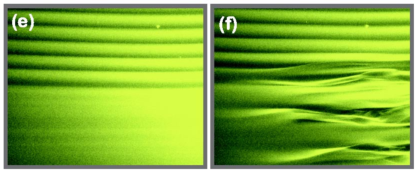
\includegraphics[width=0.49\textwidth]{./Figures/example_delay_turbulence}
  \end{center}
  \vspace{-0.5cm}
  \begin{center}
  {\tiny 'Delaying transition to turbulence by a passive mechanism', \textit{Fransson et. al.} (2006).}
  \end{center}

    \begin{itemize}
      \item Flow control: a relevant theoretical and industrial problem.
      \item Time dependence, nonlinearity, high dimensionality break many tools.
      \item Methods based on linearization often do not work.
      \item Field of active research for a long time, but famously difficult. \\~\\
    \end{itemize}
\end{frame}



\begin{frame}{Motivation 2: optimization of complex systems}
  \begin{center}
    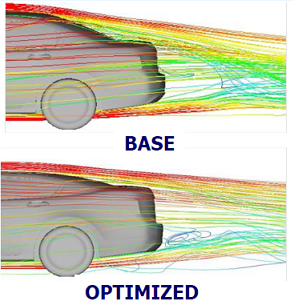
\includegraphics[width=0.25\textwidth]{./Figures/shape_opt_aero}
      \hspace{0.5cm}
    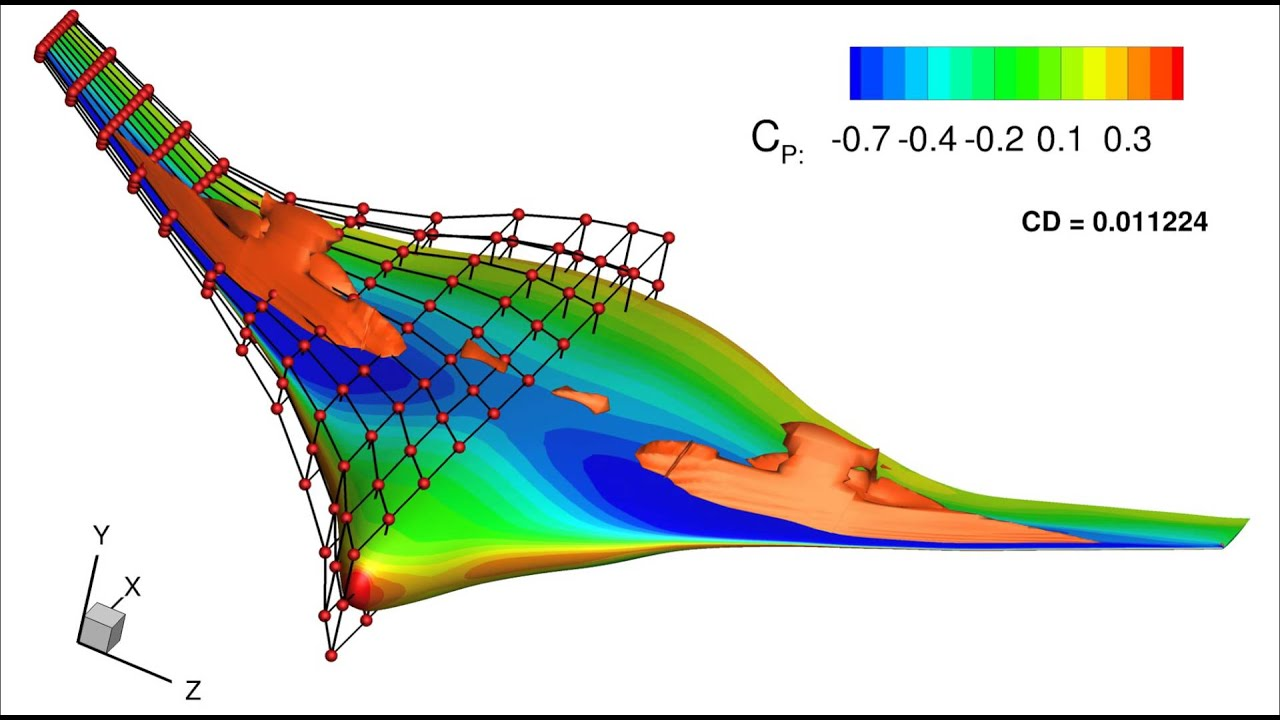
\includegraphics[width=0.40\textwidth]{./Figures/opt_shape_flying_wing}
  \end{center}

    \begin{itemize}
      \item Shape optimization: everywhere in engineering.
      \item How to optimize nonlinear problem? Challenge for gradient descent.
      \item There also, difficult, need user expertise. \\~\\
    \end{itemize}

    Try to introduce new tools? Recent successes of Deep Reinforcement Learning (DRL) on complex problems is a strong hint (Go, Poker, robotics, control of complex cooling systems). ~\\~
\end{frame}








\section{A short reminder about Artificial Neural Networks and Supervised Learning}

\begin{frame}{Artificial Neural Networks: a bit of history}
    \begin{center}
    Idea of ANNs appeared with the first computers: \\
    \end{center}
    'The perceptron, a perceiving and recognizing automaton', \textit{Rosenblatt}, Cornell Aeronautical Laboratory (1957). \\

    \begin{center}
      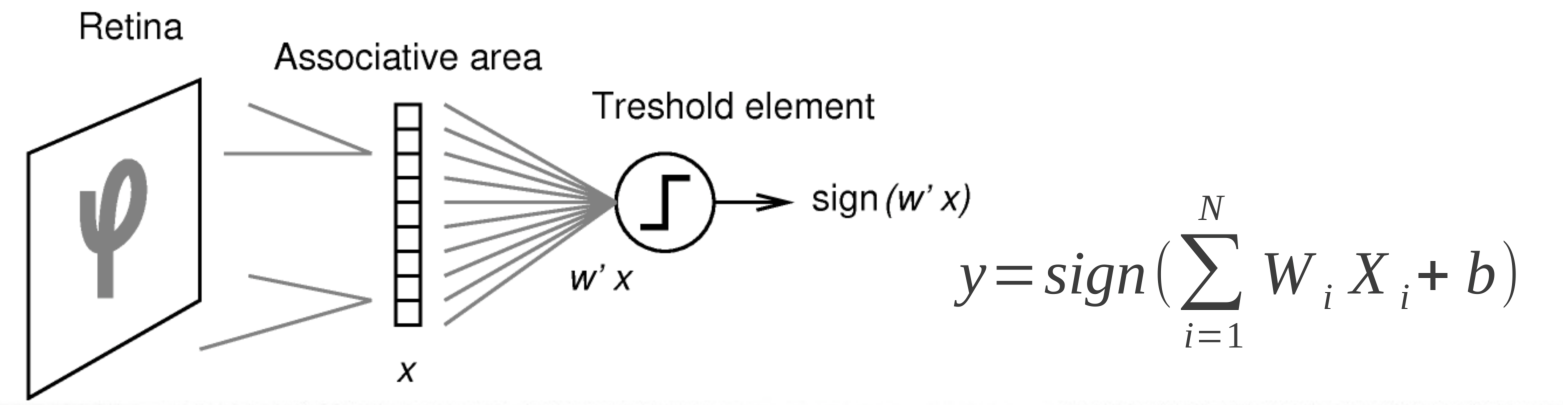
\includegraphics[width=0.8\textwidth]{./Figures/ANNs_supervised_learning/perceptron}
    \end{center}

    It took some time before useful applications:

    \begin{itemize}
      \item A few applications during the 70s.
      \item Large scale application of CNNs in the 90s.
      \item Recently 'AI spring' since around 2012: Deep Learning.
    \end{itemize}

    Succession of 'AI springs' and 'AI winters', but now it is summer...
\end{frame}



\begin{frame}{Deep ANNs: I}
    Artificial Neural Networks are simply a set of neurons.

    \begin{center}
      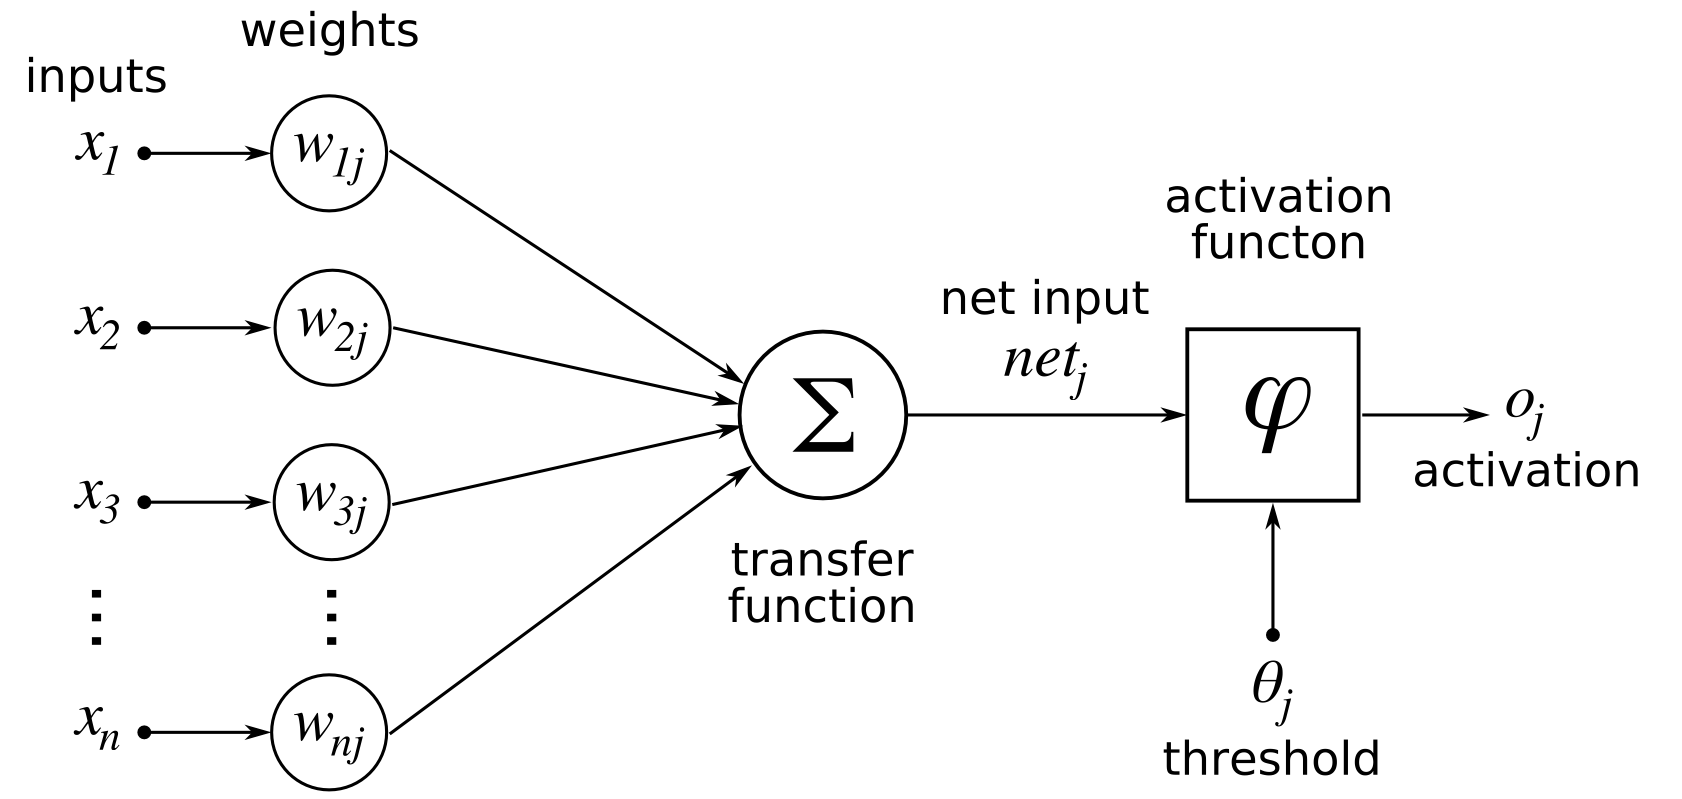
\includegraphics[width=0.43\textwidth]{./Figures/ANNs_supervised_learning/ArtificialNeuronModel_english}
      \hspace{0.1cm}
      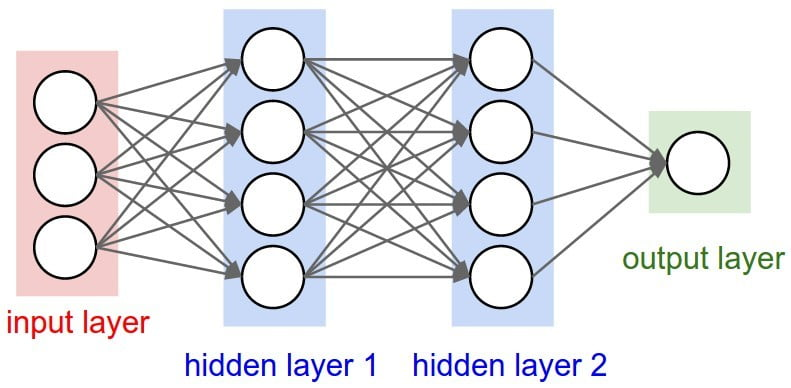
\includegraphics[width=0.43\textwidth]{./Figures/ANNs_supervised_learning/artificial_neural_network_1-791x388}
    \end{center}

    Deep ANNs: ANNs with several hidden layers. Feed one layer in the next: 'Deep Learning', \textit{LeCun et. al.}, Nature (2015). \\~\\

    Convolution layers enforce invariance by translation:

    \begin{center}
      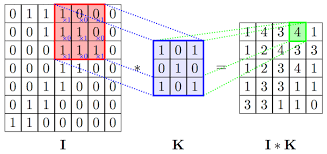
\includegraphics[width=0.42\textwidth]{./Figures/ANNs_supervised_learning/convolutional_layer}
    \end{center}
\end{frame}



\begin{frame}{Deep ANNs: II}
    What activation function to use?

    \begin{center}
      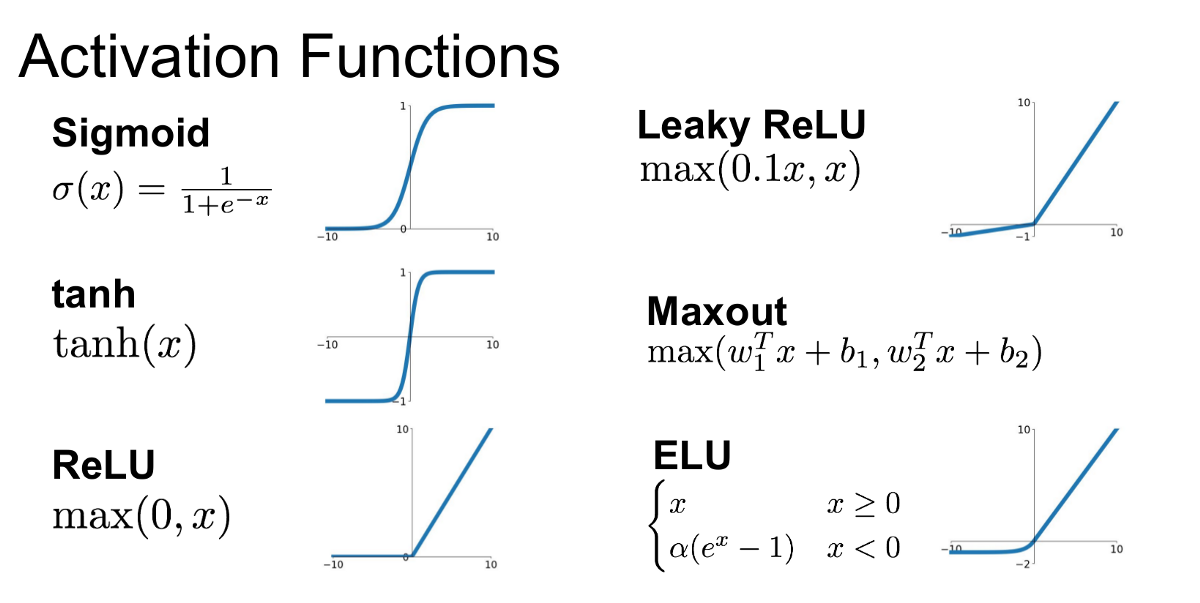
\includegraphics[width=0.7\textwidth]{./Figures/ANNs_supervised_learning/activation_functions}
    \end{center}

    \begin{itemize}
      \item Linear activation function: only linear network...
      \item Non linear functions: in practice (leaky) ReLU often best.
    \end{itemize}

    Deep ANN + non linear activation function = universal approximator. 'Multilayer feedforward networks are universal approximators', \textit{Hornik et. al.}, Neural Networks (1989). Universal mapping.
\end{frame}


\begin{frame}{Deep ANNs: III}
    What architecture to use?

    \begin{itemize}
        \item In theory, 1-layer is enough to be universal approximator.
        \item In practice, advantage of depth, invariance by translation, etc. \\~\\
    \end{itemize}

    Example of XOR function, N inputs:

    \begin{itemize}
        \item Need order $2^N$ neurons if 1 layer.
        \item Need order $N$ neurons if $log(N)$ layers. \\~\\
    \end{itemize}

    Example of CNNs for image analysis: re-use the weights:


    \begin{center}
      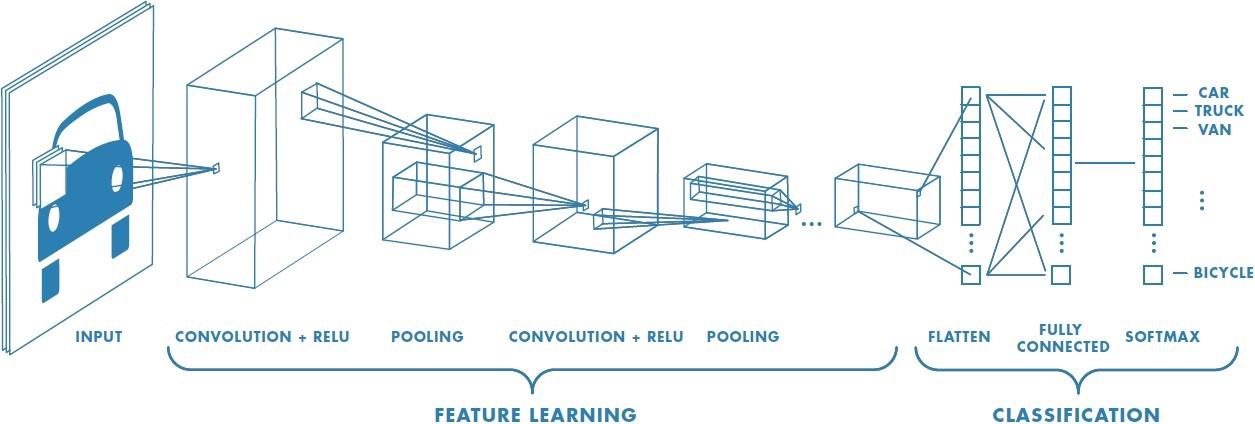
\includegraphics[width=0.7\textwidth]{./Figures/deepCNN}
    \end{center}
\end{frame}



\begin{frame}{Deep ANNs: IV}
    Universal approximator, easily parallelizable, effective representation \\

    \begin{center}
       How to train?
    \end{center}

    \begin{itemize}
      \item Naive method: try at random....
      \item Better method: gradient descent, back propagation of errors: 'Applications of advances in nonlinear sensitivity analysis', \textit{Werbos}, System modeling and optimization (1982).
    \end{itemize}

    \begin{center}
      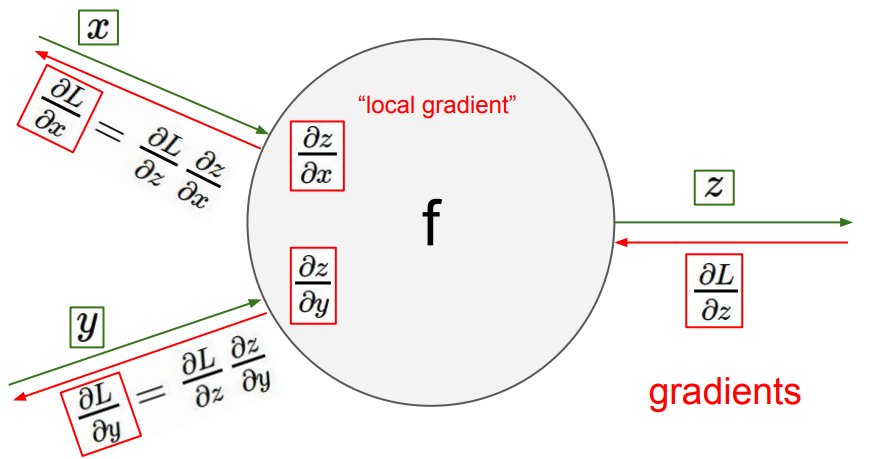
\includegraphics[width=0.38\textwidth]{./Figures/ANNs_supervised_learning/back_prop}
    \end{center}

    \begin{itemize}
      \item Feed data in, compute error.
      \item Back propagate (Leibniz) the error gradient.
      \item Update the coefficients.
    \end{itemize}
\end{frame}


\begin{frame}{Deep ANNs: V}
    Still problems training: overfitting, stability of gradient, etc.

    \begin{itemize}
        \item Large datasets, training vs. validation, data augmentation.
        \item Dropout layers (drop connections at random).
        \item Weight initialization for gradient stability.
        \item Batch renormalization (fix mean and variance in each layer).
        \item Residual networks (learn changes from identity).
    \end{itemize}

    \begin{center}
      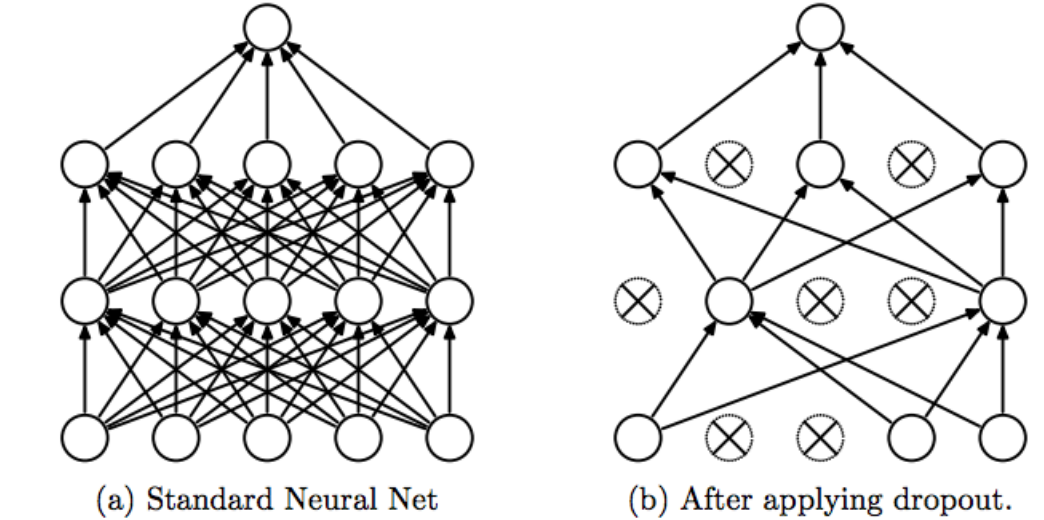
\includegraphics[width=0.38\textwidth]{./Figures/dropout}
        \hspace{0.5cm}
      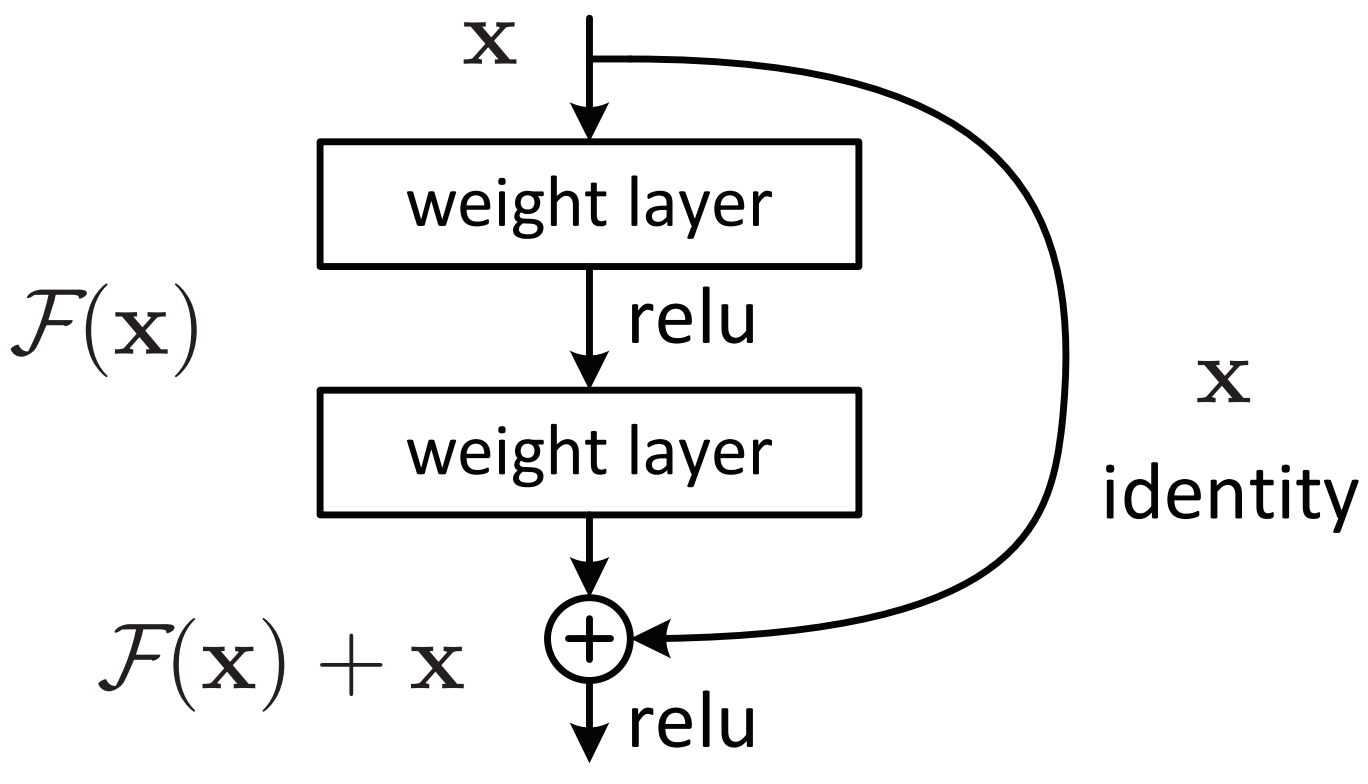
\includegraphics[width=0.42\textwidth]{./Figures/resnet_layer}
    \end{center}

\end{frame}



\begin{frame}{The Deep Learning revolution}
    \begin{itemize}
      \item Large amounts of data, powerful GPUs, fast batch training.
      \item A number of technical tricks, many beautiful / interesting results...
    \end{itemize}

    "A Neural Algorithm of Artistic Style", Gatys et. al., ArXiv (2015).
    "Explaining and Harnessing Adversarial Examples", Goodfellow et. al., ICLR 2015.

    \begin{center}
      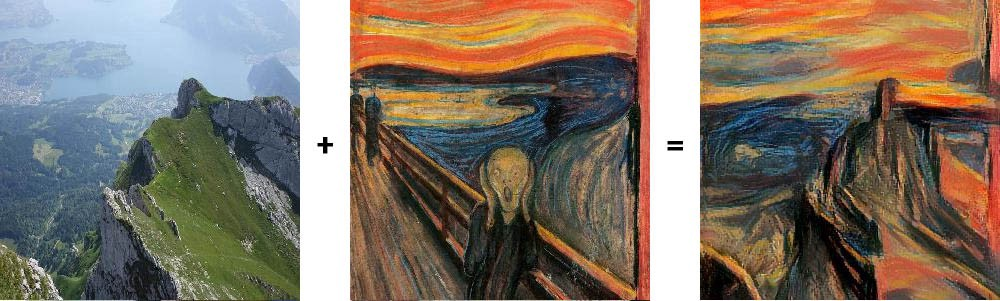
\includegraphics[width=0.55\textwidth]{./Figures/style_transfer} \\~\\
      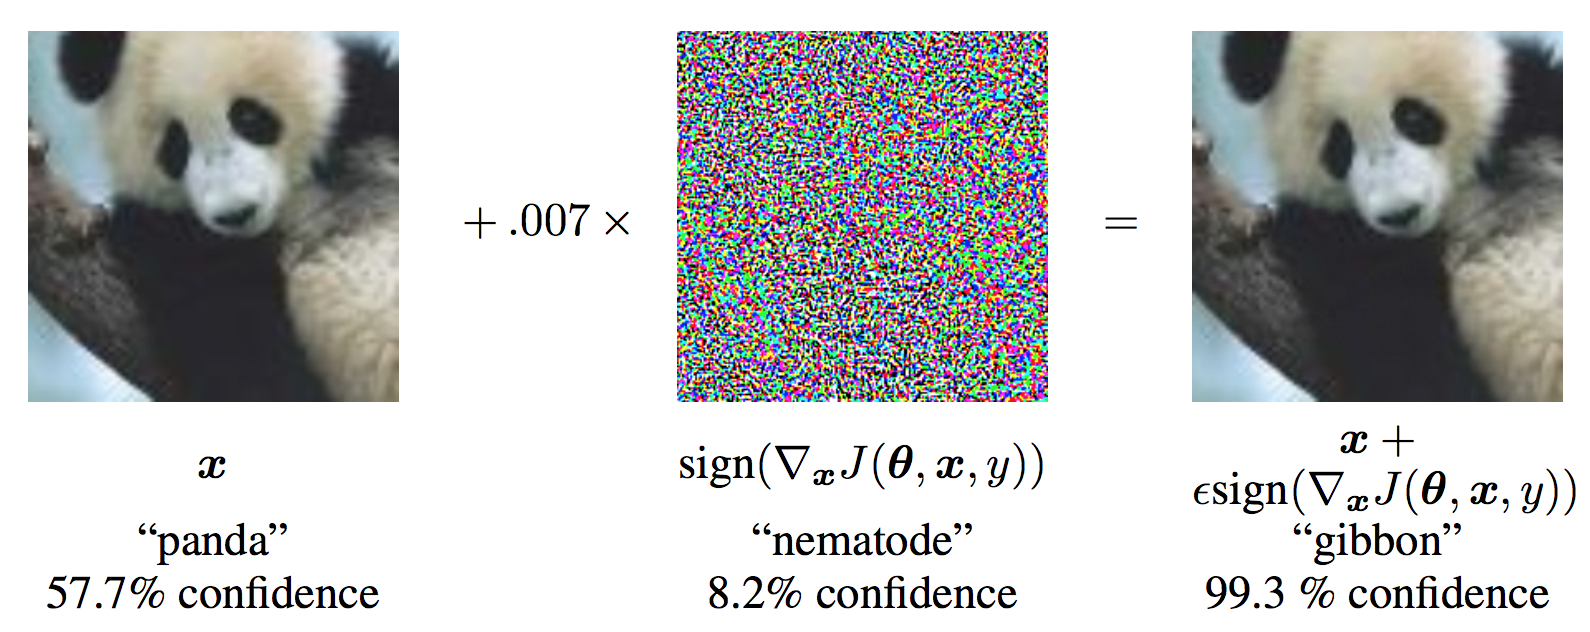
\includegraphics[width=0.55\textwidth]{./Figures/adversarial}
    \end{center}
\end{frame}

\begin{frame}{Supervised learning: describe a function from examples}

    \begin{center}
      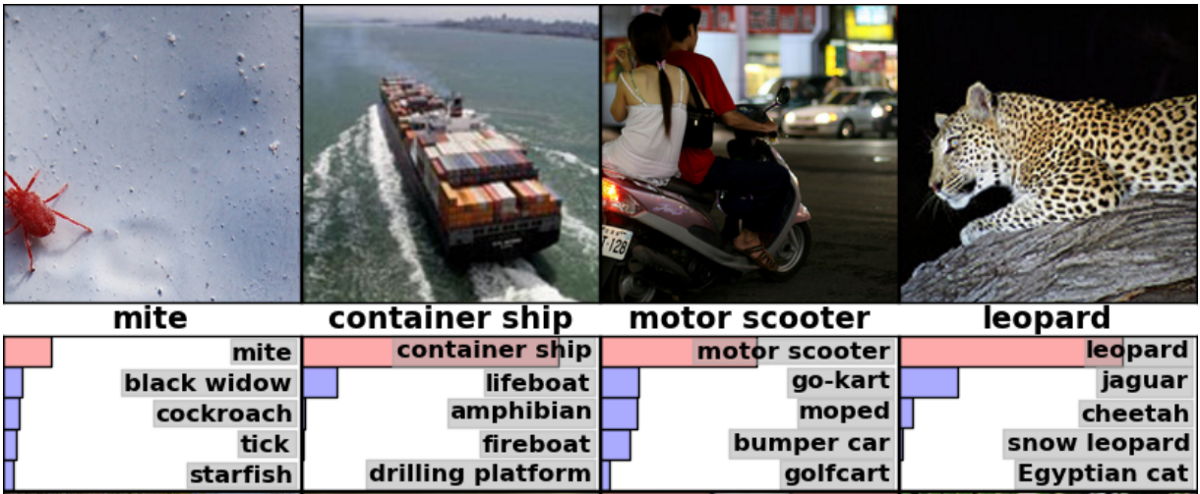
\includegraphics[width=0.55\textwidth]{./Figures/ANNs_supervised_learning/classification}
      \hspace{0.1cm}
      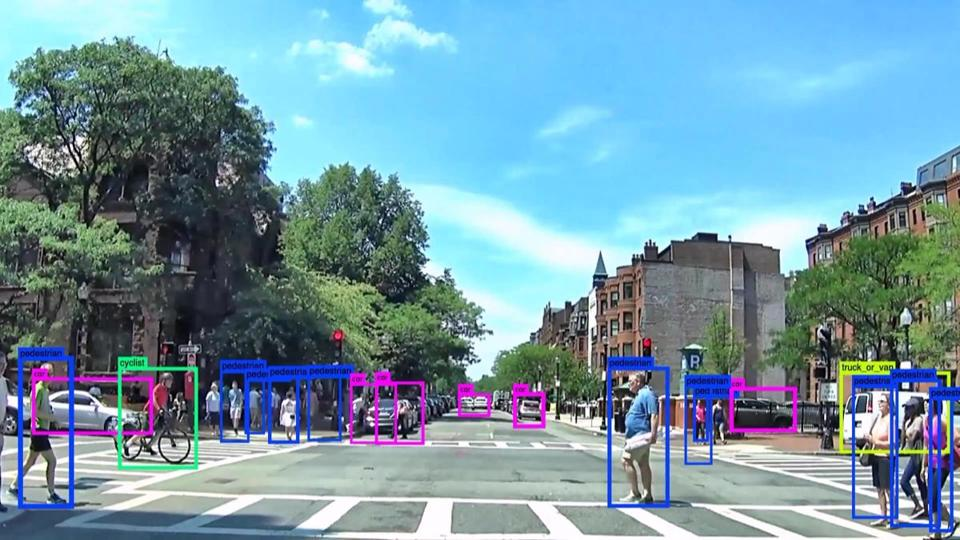
\includegraphics[width=0.42\textwidth]{./Figures/ANNs_supervised_learning/Neurala_AutoRecognition-08}
    \end{center}

    \begin{center}
    Supervised learning, image analysis work...
    \end{center}

    \begin{center}
      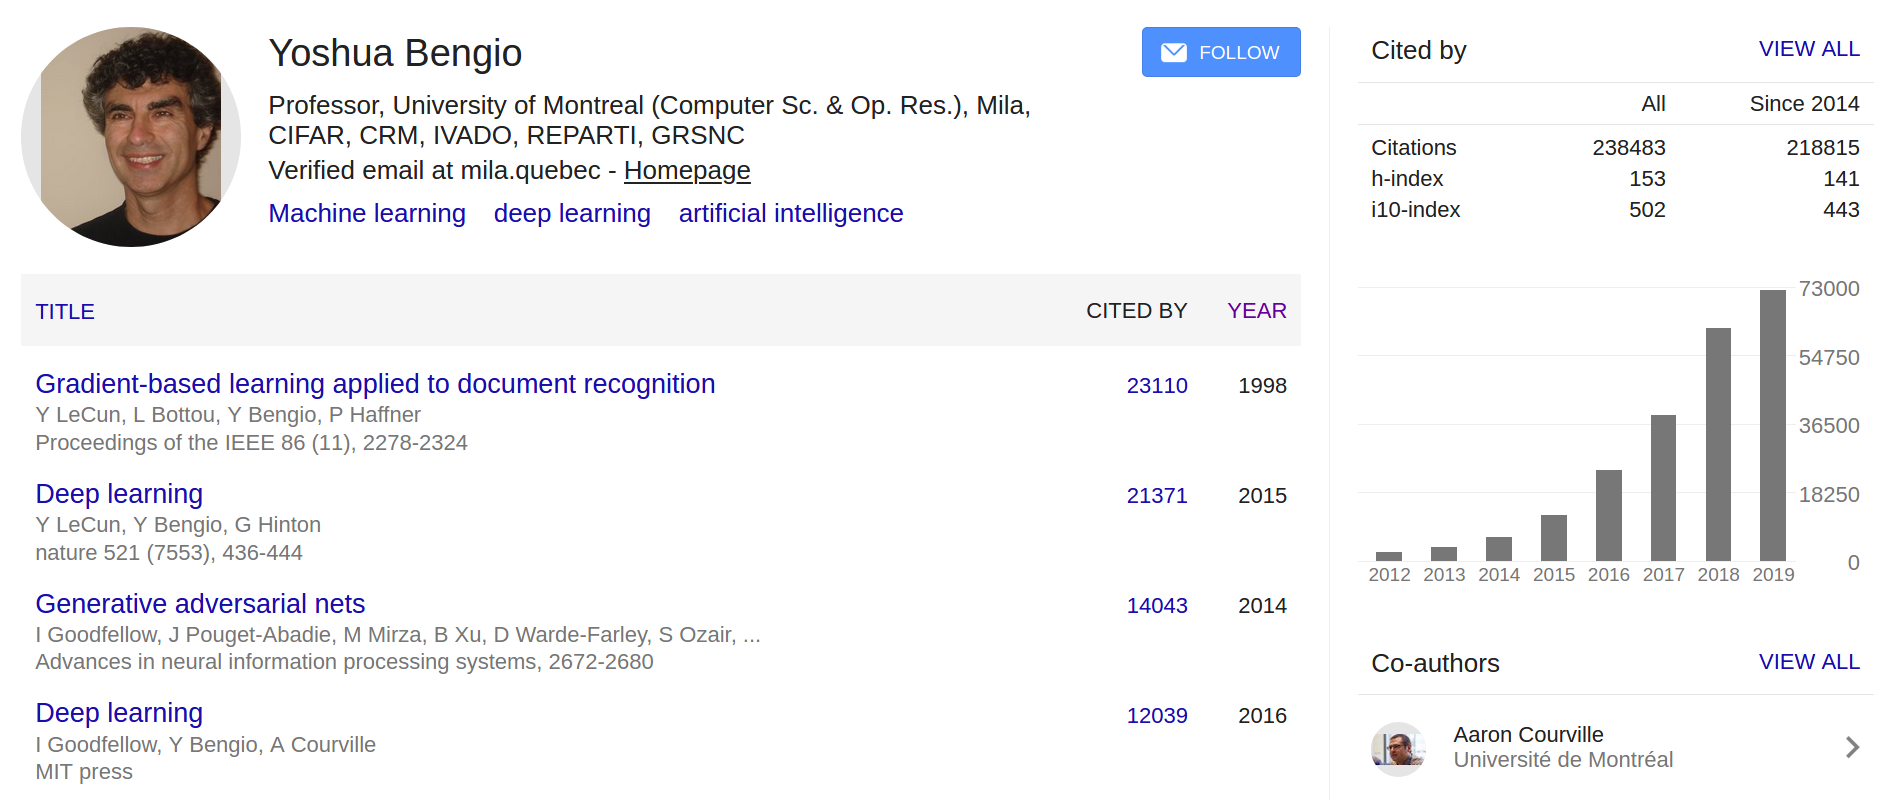
\includegraphics[width=0.8\textwidth]{./Figures/ANNs_supervised_learning/yoshua_bengio}
    \end{center}

\end{frame}













\section{From Supervised to Reinforcement Learning}

\begin{frame}{Reinforcement Learning}
  % What if do not know the solution? Train the ANN through experimentation with the environment to control.
  How to learn when no solution is known? Learn by trial and error.

    \begin{center}
    'A review on Deep Reinforcement Learning for Fluid Mechanics', Garnier et. al., ArXiv (2019).
    \end{center}

  \begin{center}
      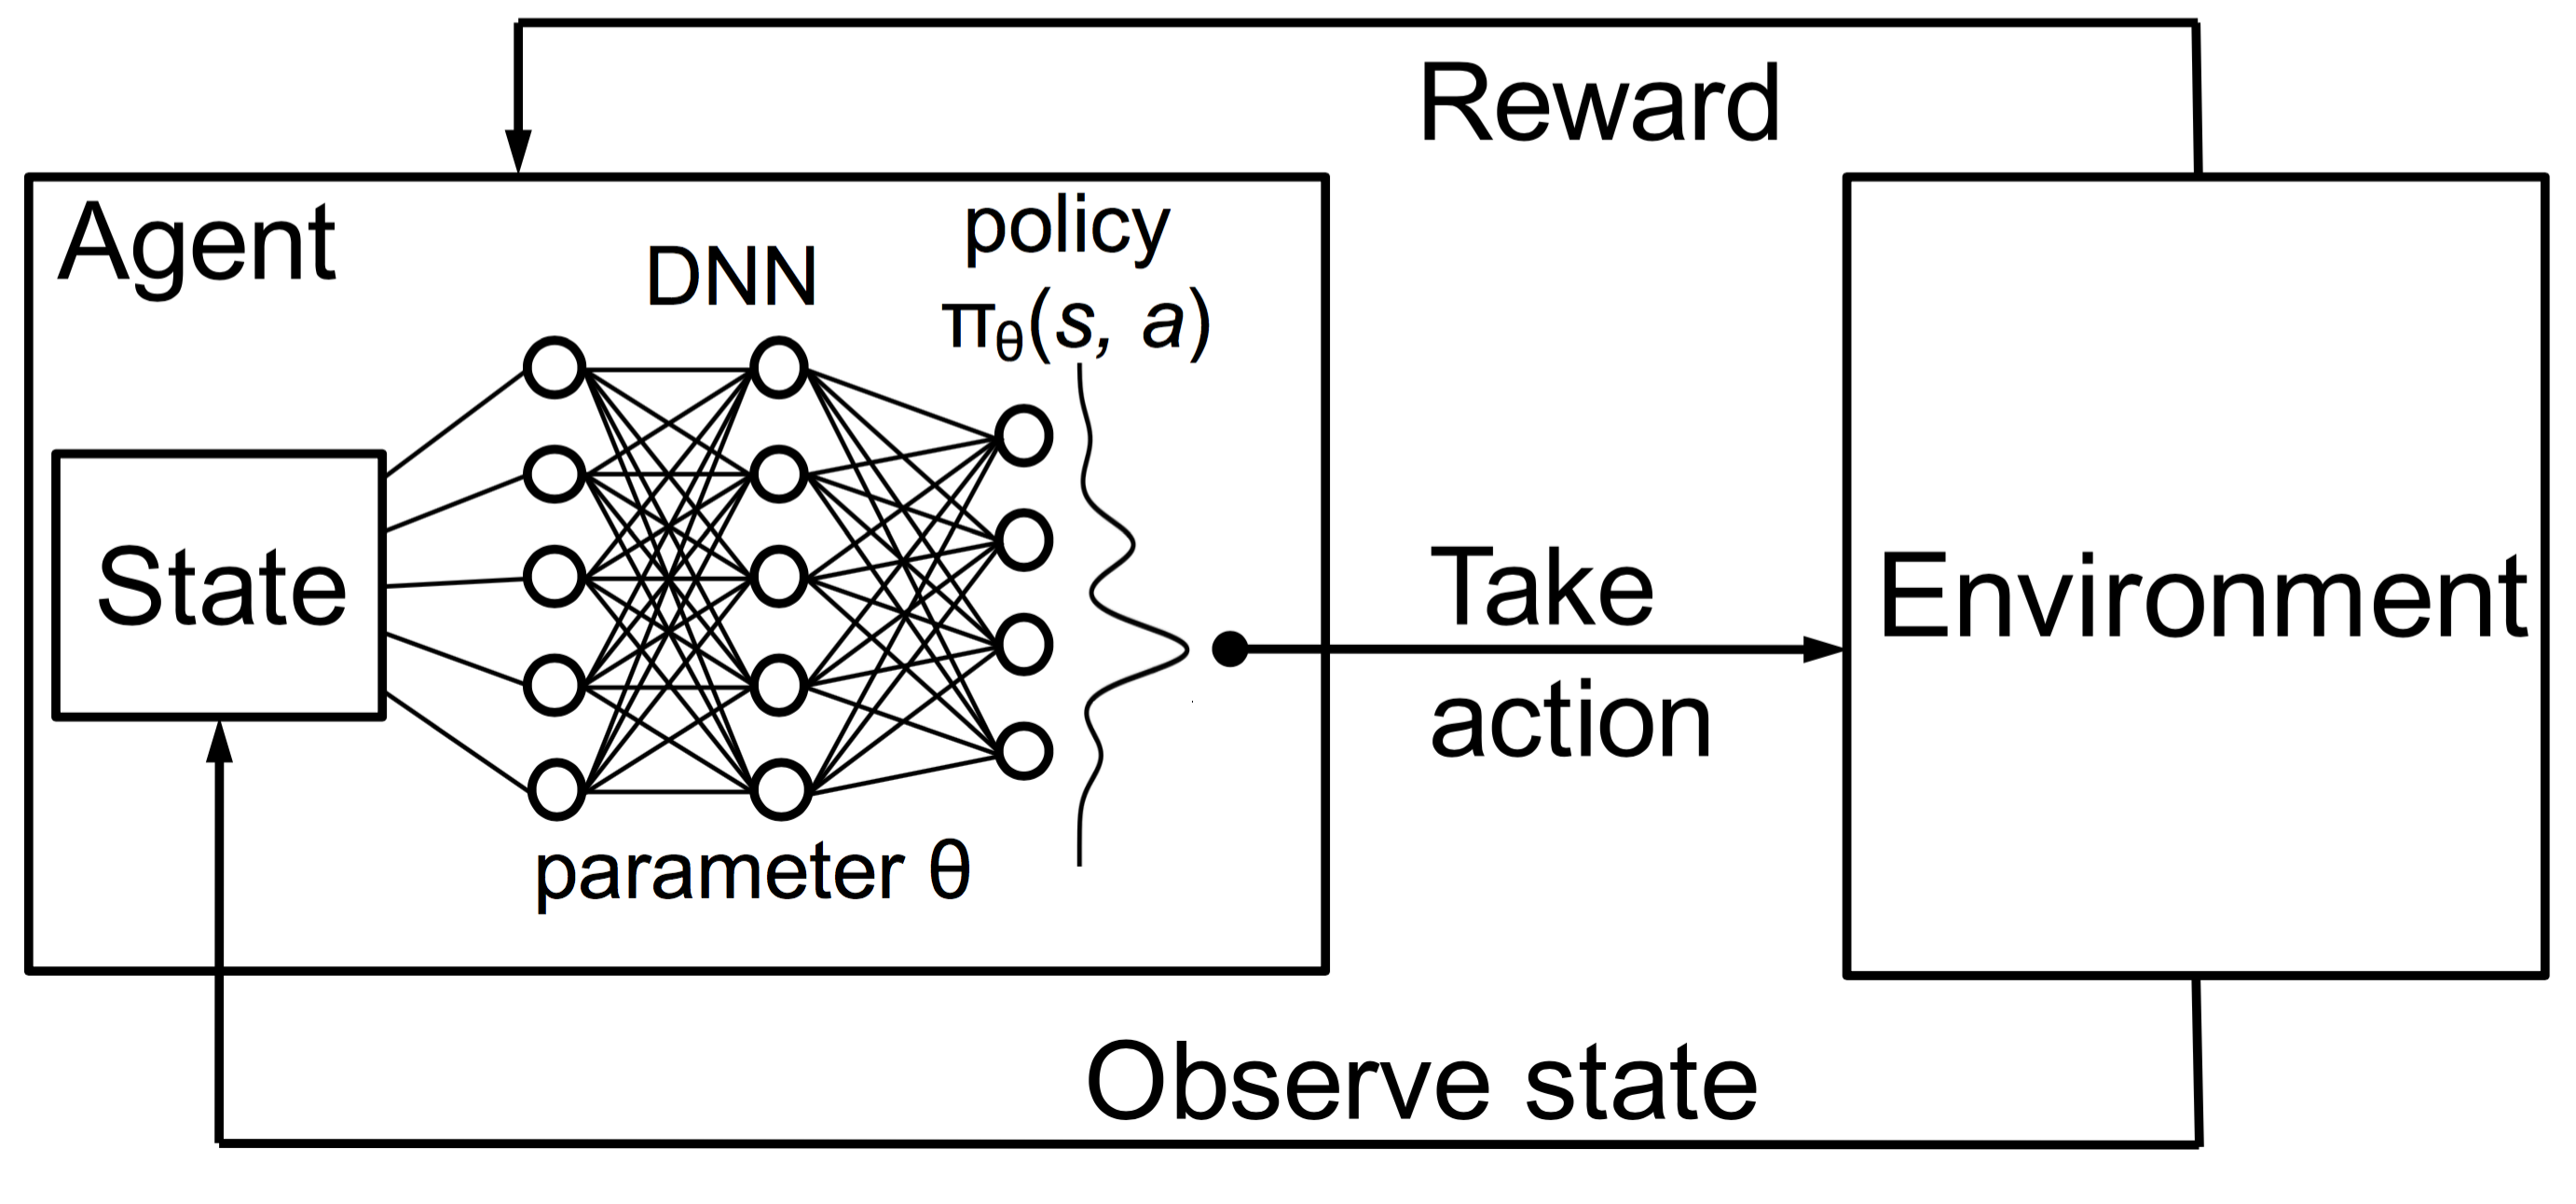
\includegraphics[width=0.6\textwidth]{./Figures/fig_DRL_policy.png}
  \end{center}

  $s$ the state, $a$ action, $r$ reward, policy $\pi(a | s)$ the probability of $a$ in $s$. \\~\\

   Several methods. Main ones:
   
   \begin{itemize}
     \item Q-learning.
     \item Policy gradients.
   \end{itemize}
\end{frame}

\section{i. Q-learning}

\begin{frame}{Q-Learning (I)}
    \begin{center}
      'Human-level control through deep reinforcement learning', \textit{Mnih et. al.}, Nature (2015). \\
    \end{center}

    \begin{center}
      Based on older work about Q-Learning: \\ 'Q-learning', \textit{Watkins et. al.}, Machine Learning (1992). \\~\\
    \end{center}

    Discounted future reward: $R_t = r_t + \gamma r_{t+1} + \gamma^2 r_{t+2} + ... = r_t + \gamma R_{t+1}$. \\~\\

    Given a state $s$ and a policy $\pi$ define the value function: \\
    $$V^{\pi}(s) = \mathbb{E} \left( \sum_{t \geq 0} \gamma^t r_t | s, \pi \right),$$

    and the optimal value function: $V^{*}(s) = \max_{\pi} V^{\pi}(s)$.
\end{frame}



\begin{frame}{Q-Learning (II)}
    Introduce the action of the agent: expected return, starting in state $s$, performing action $a$, continuing with policy $\pi$: $Q^{\pi}(s, a)$. \\~\\

    Then: $Q^{*} = \max_{\pi} Q^{\pi}(s, a)$, and $V^{*}(s) = \max_{a} Q^{*}(s, a)$. Finally:

    $$\pi^{*}(s) = \argmax_{a} Q^{*}(s, a).$$

    Therefore, knowledge of $Q^{*}$ is knowledge of $\pi^{*}$. Q learning: iterative approximation of $Q^{*}$ using the Bellman equation:

    $$ Q^{*}(s, a) = r + \gamma \max_{a'} Q^{*}(s', a').$$

    Random action at probability $\epsilon$, $\argmax$ action at probability $1 - \epsilon$, and:
    $$Q_{n+1}(s_t, a_t) = Q_n(s_t, a_t) + \alpha (r_{t+1} + \gamma \max_{a} Q_n(s_{t+1}, a) - Q_n(s_t, a_t)).$$
    
    This kind of techniques also known as 'dynamic programming': break a problem in succession of small sub-problems.
\end{frame}



\begin{frame}{Q-learning on an example}
    Simple example: a 2 x 2 matrix game.

    \begin{center}
      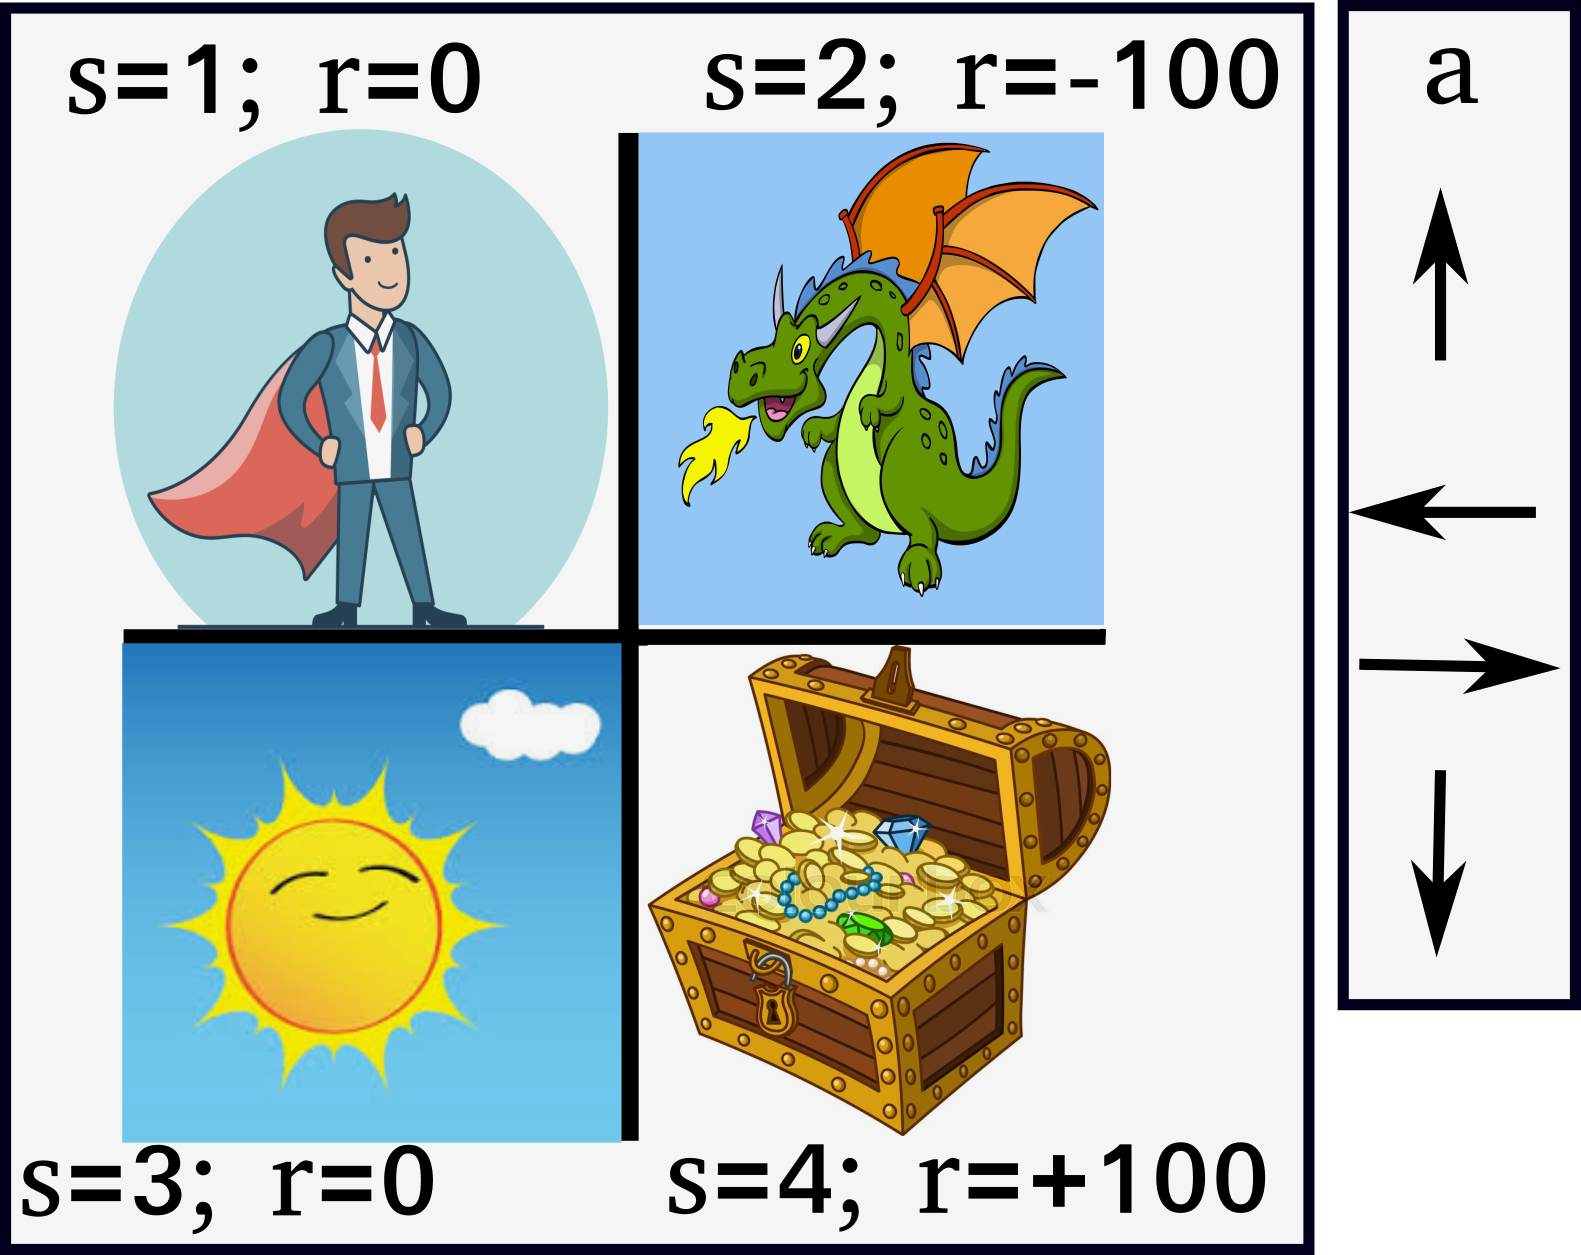
\includegraphics[width=0.35\textwidth]{./Figures/ANNs_reinforcement_learning/Q_learning_example}
    \end{center}

    What does $Q^{*}(s, a)$ look like? First a bit of initialization:

    \begin{center}
      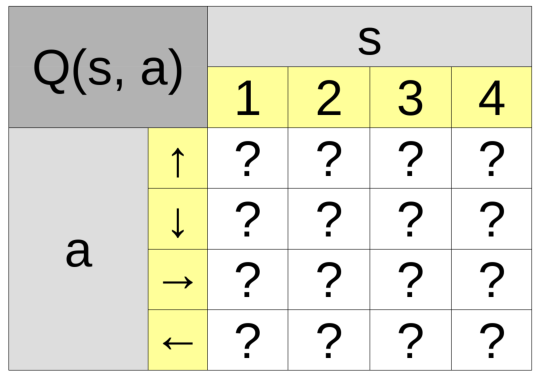
\includegraphics[width=0.35\textwidth]{./Figures/ANNs_reinforcement_learning/Q_learning_example_mat}
      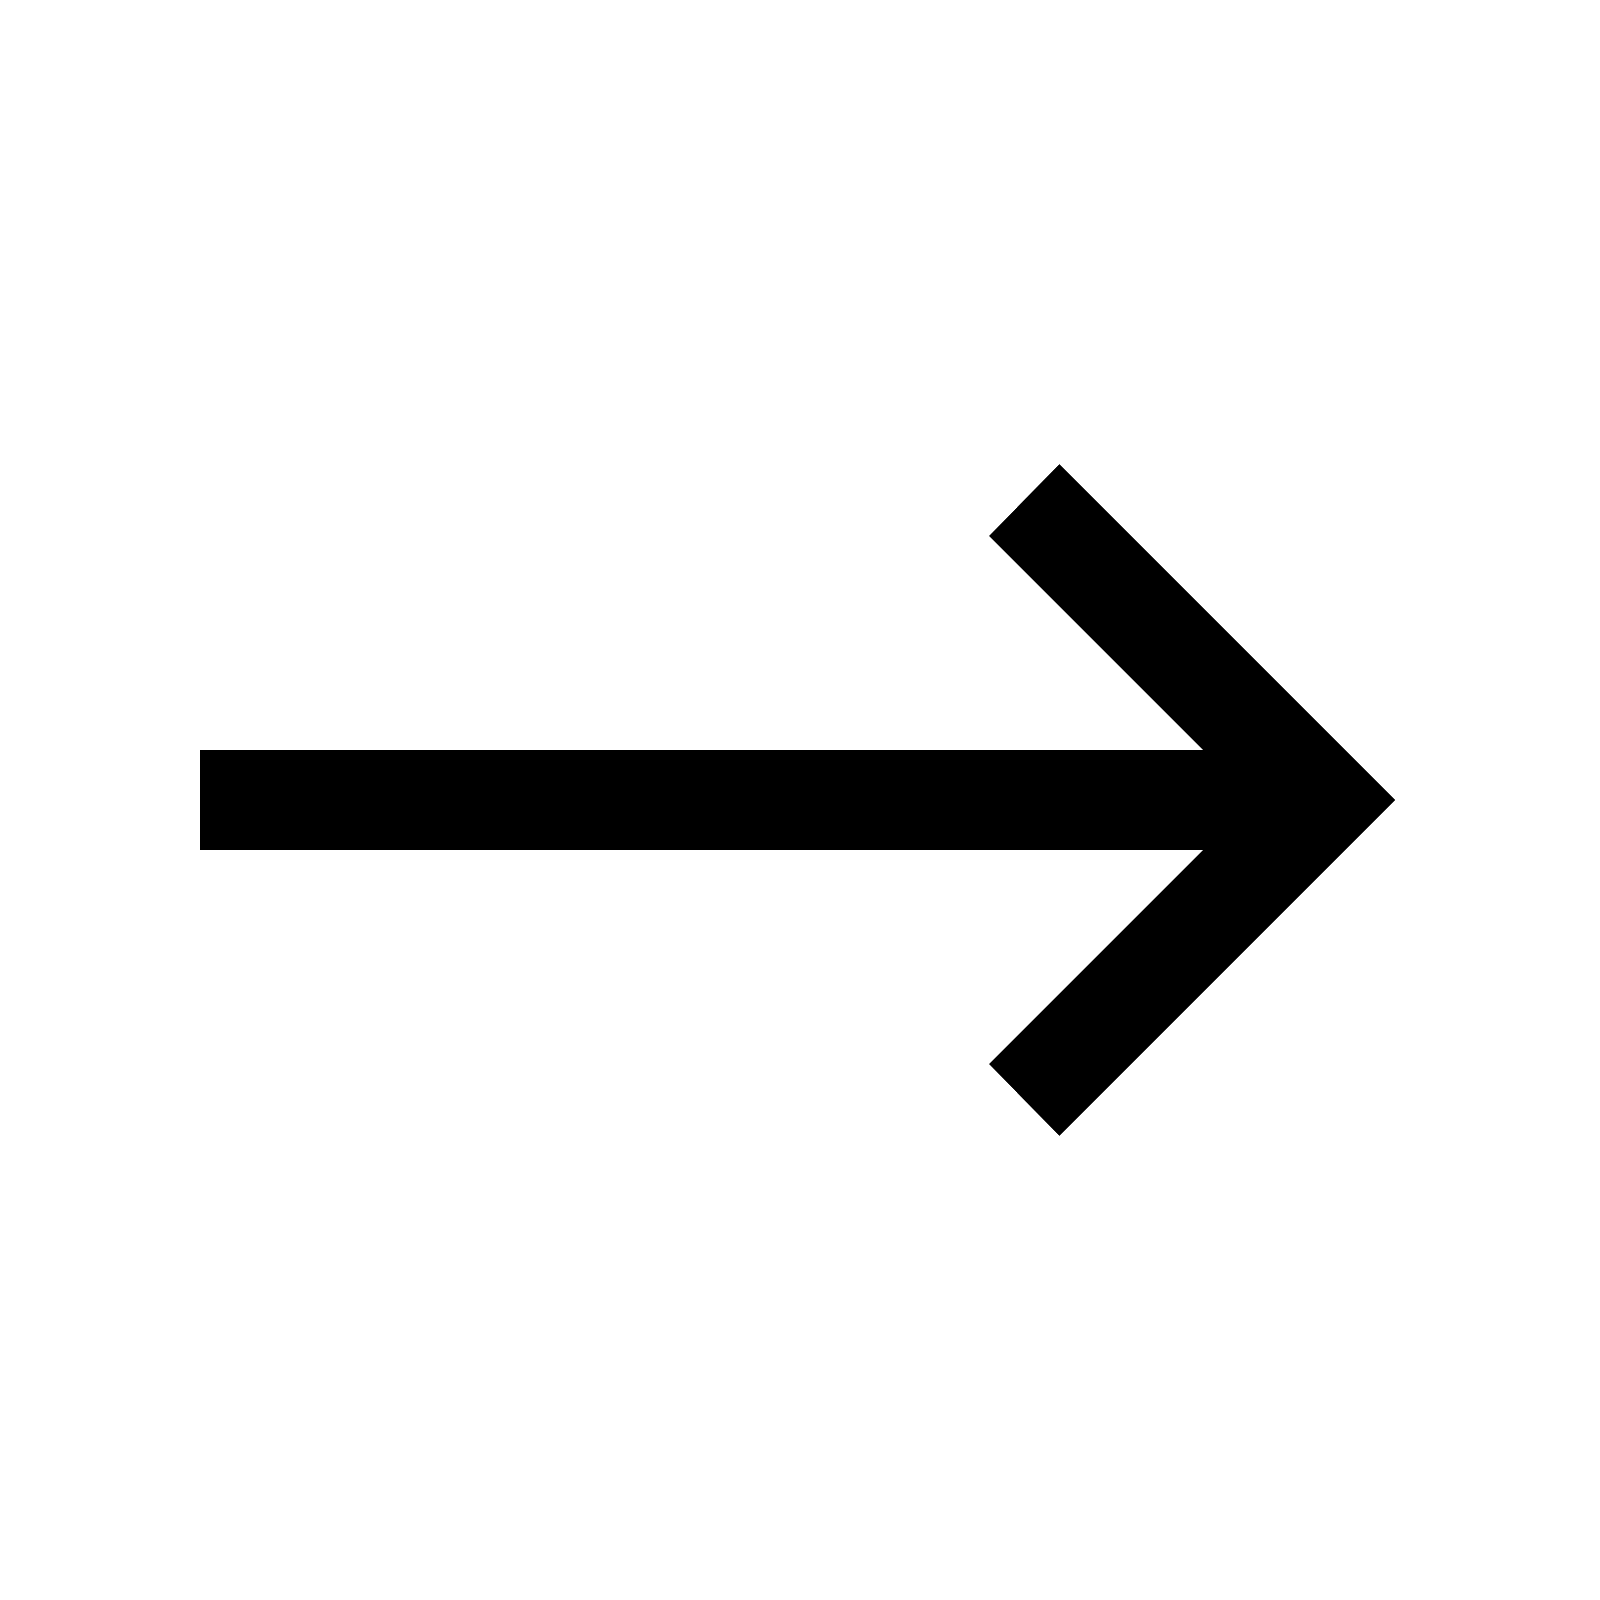
\includegraphics[width=0.05\textwidth]{./Figures/ANNs_reinforcement_learning/arrow_right}
      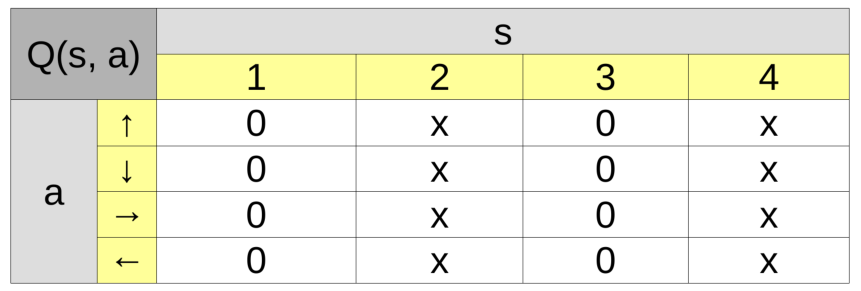
\includegraphics[width=0.55\textwidth]{./Figures/ANNs_reinforcement_learning/Q_learning_example_0}
    \end{center}
\end{frame}



\begin{frame}{Q-learning on an example}
    Simple example: a 2 x 2 matrix game.

    \begin{center}
      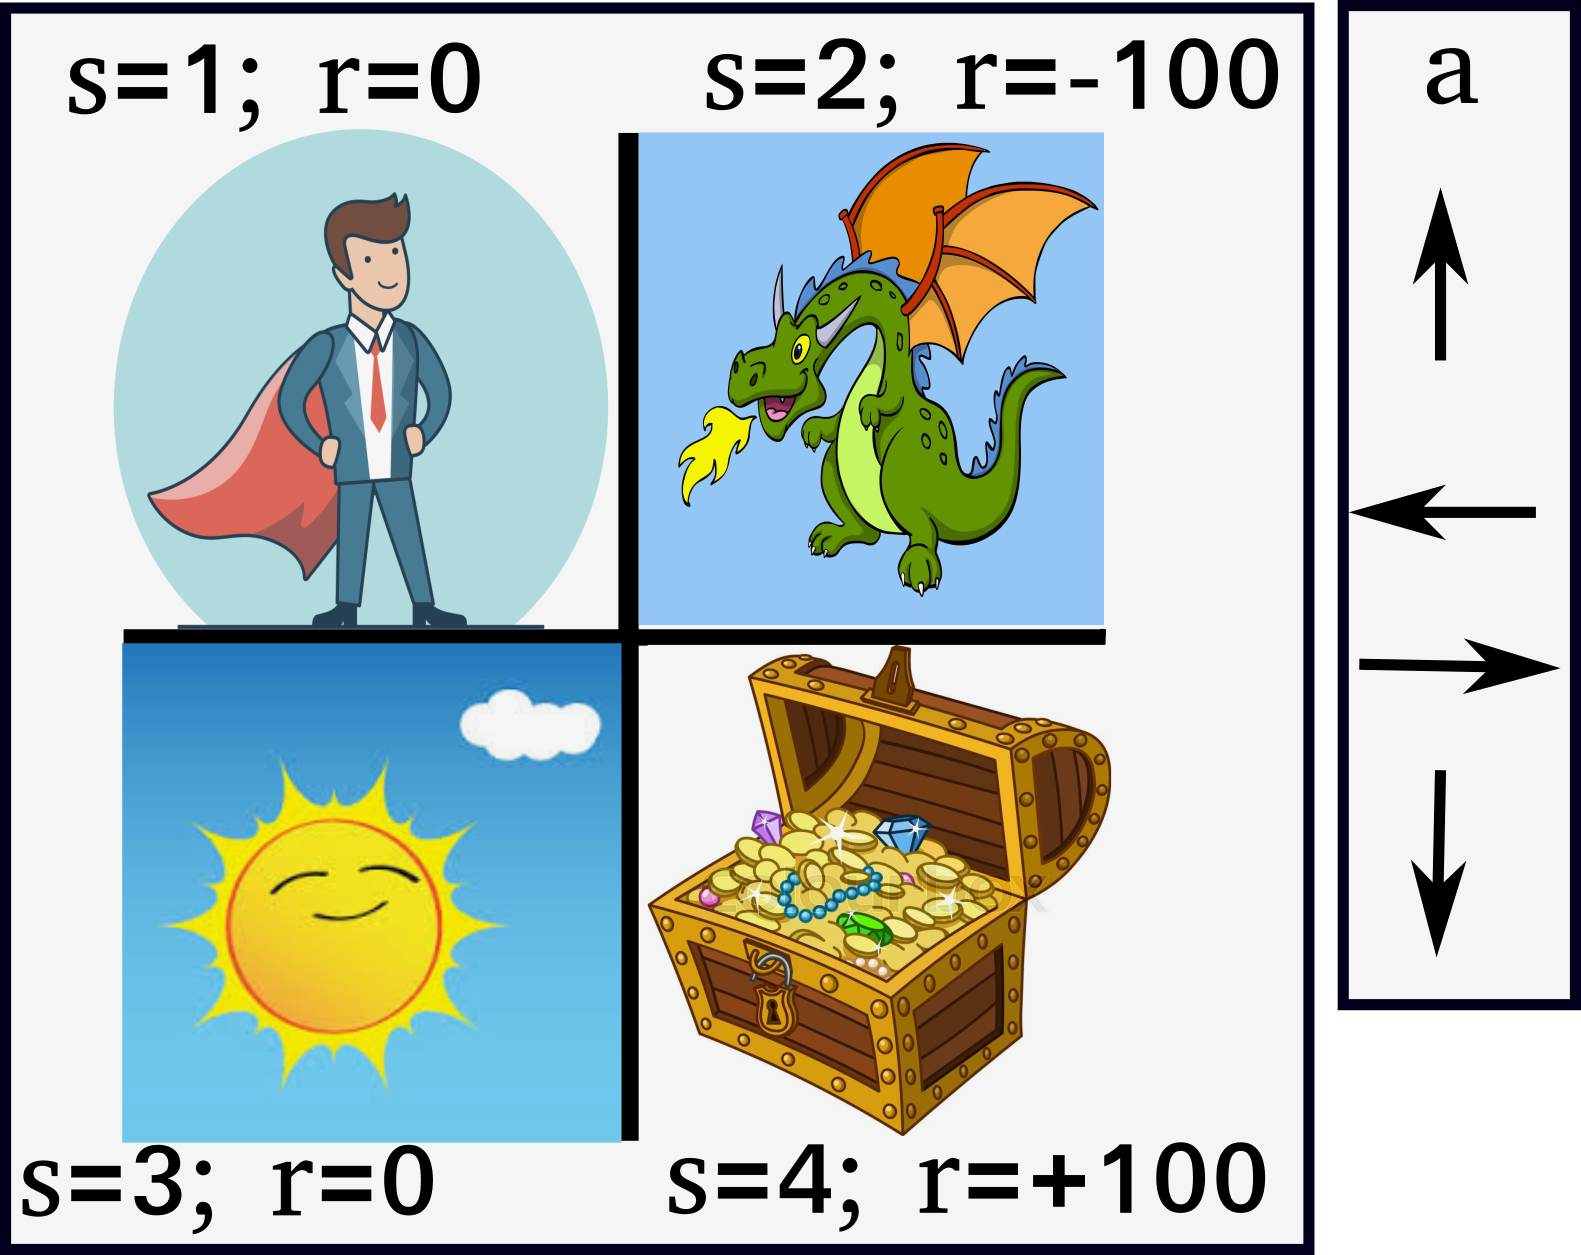
\includegraphics[width=0.35\textwidth]{./Figures/ANNs_reinforcement_learning/Q_learning_example}
    \end{center}

    What does $Q^{*}(s, a)$ look like? Now learn, use $\alpha = 0.1$, $\gamma = 0.5$, $\epsilon = 1$: r.

    \begin{center}
      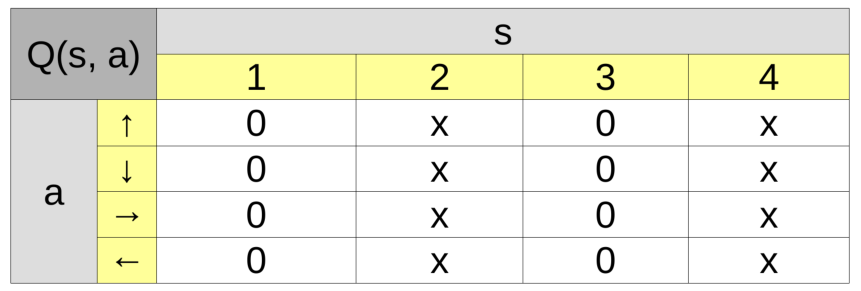
\includegraphics[width=0.46\textwidth]{./Figures/ANNs_reinforcement_learning/Q_learning_example_0}
      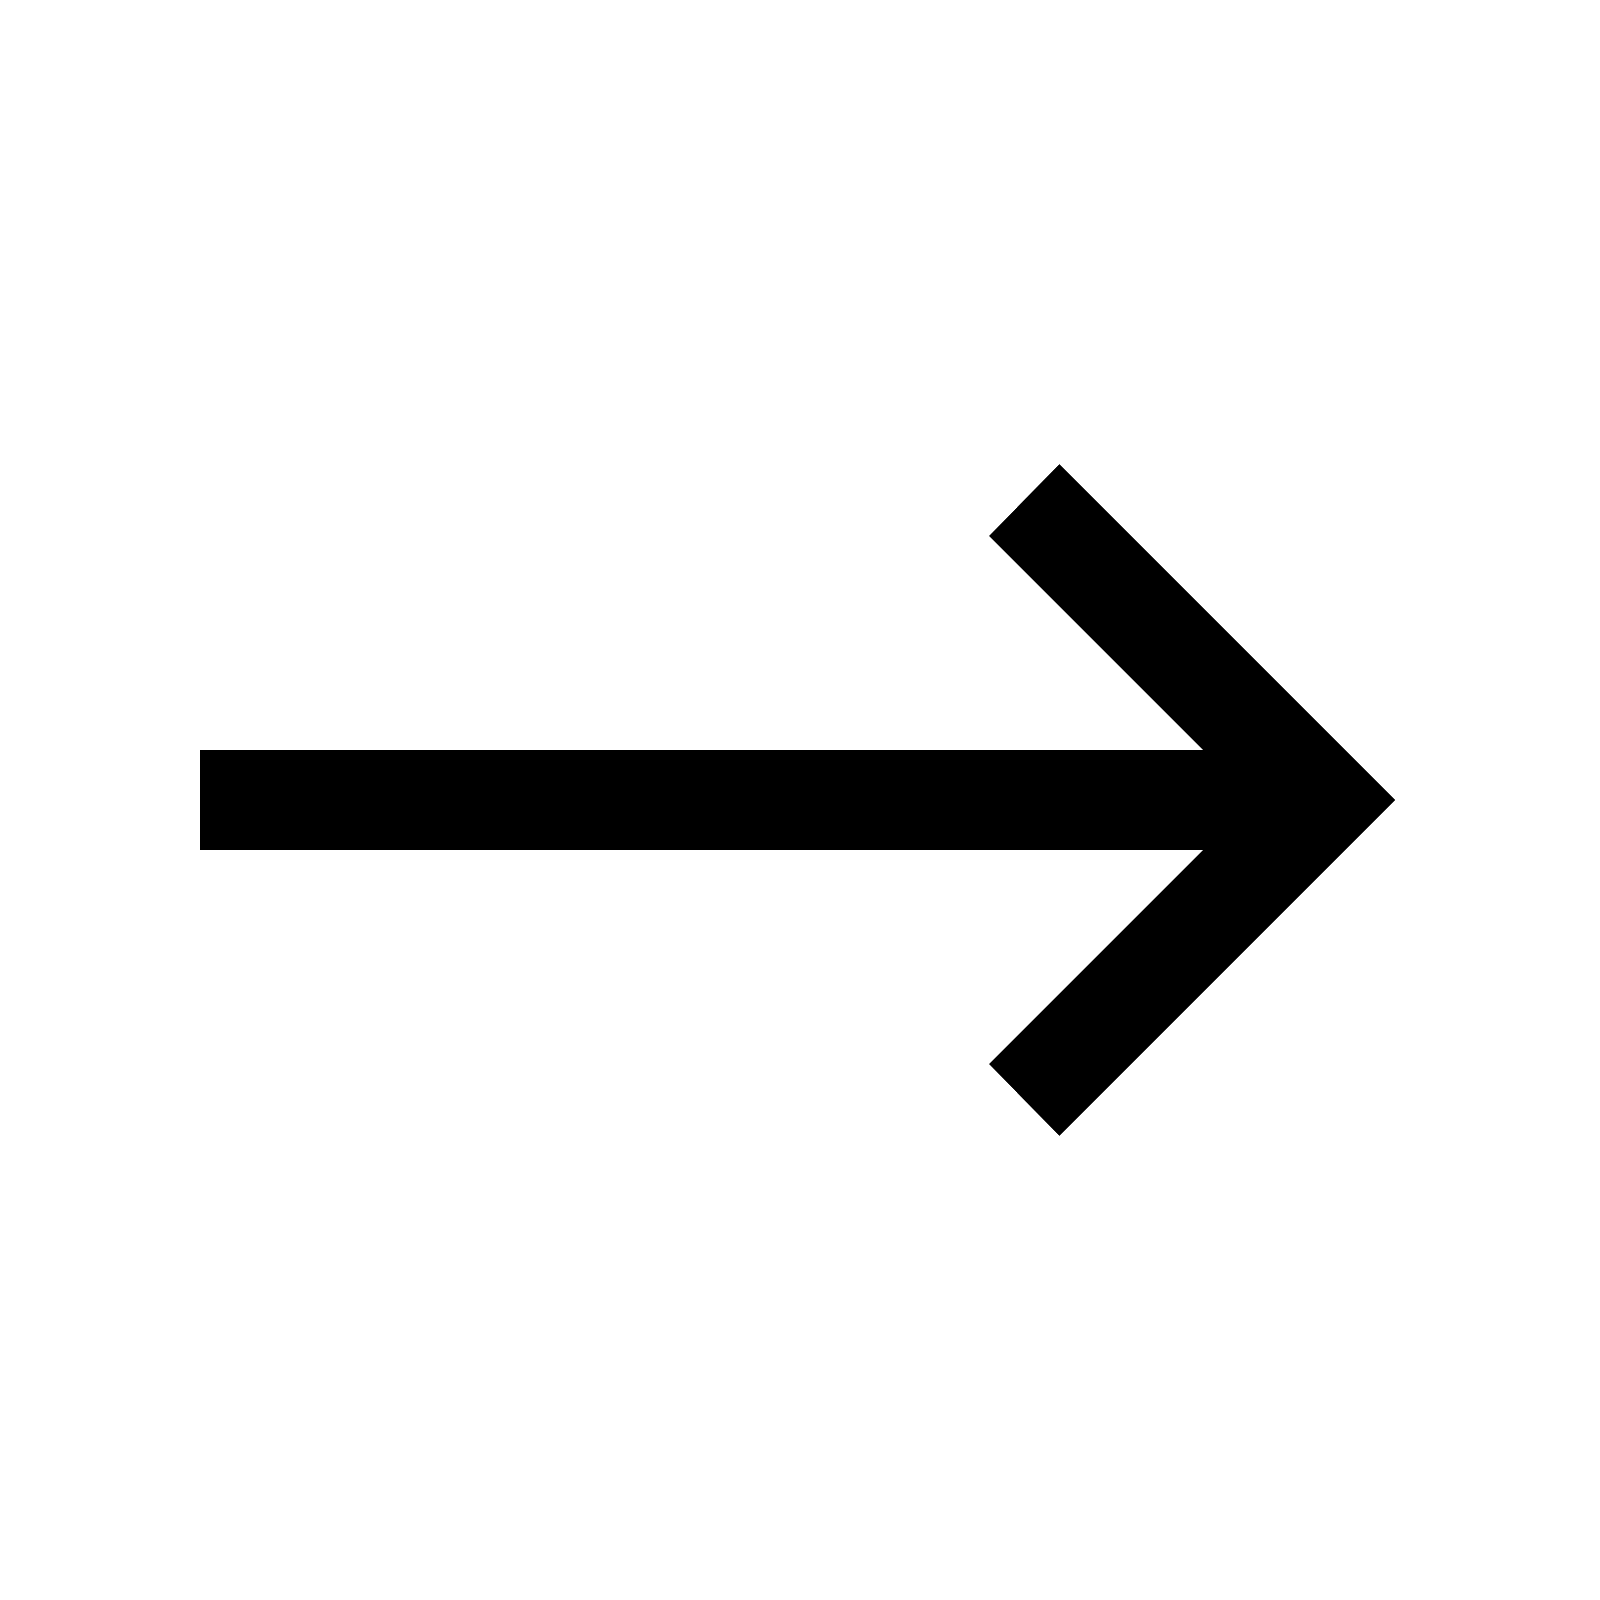
\includegraphics[width=0.05\textwidth]{./Figures/ANNs_reinforcement_learning/arrow_right}
      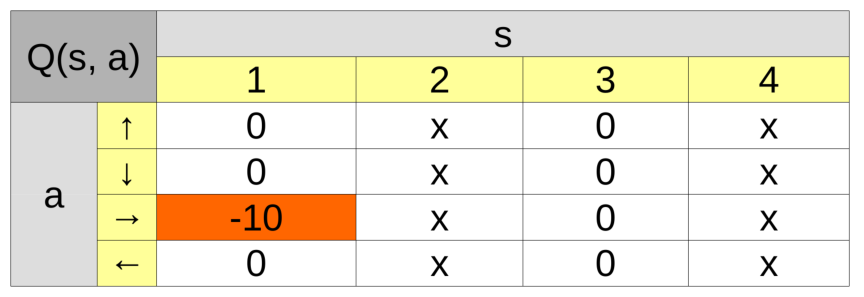
\includegraphics[width=0.46\textwidth]{./Figures/ANNs_reinforcement_learning/Q_learning_example_1}
    \end{center}
\end{frame}



\begin{frame}{Q-learning on an example}
    Simple example: a 2 x 2 matrix game.

    \begin{center}
      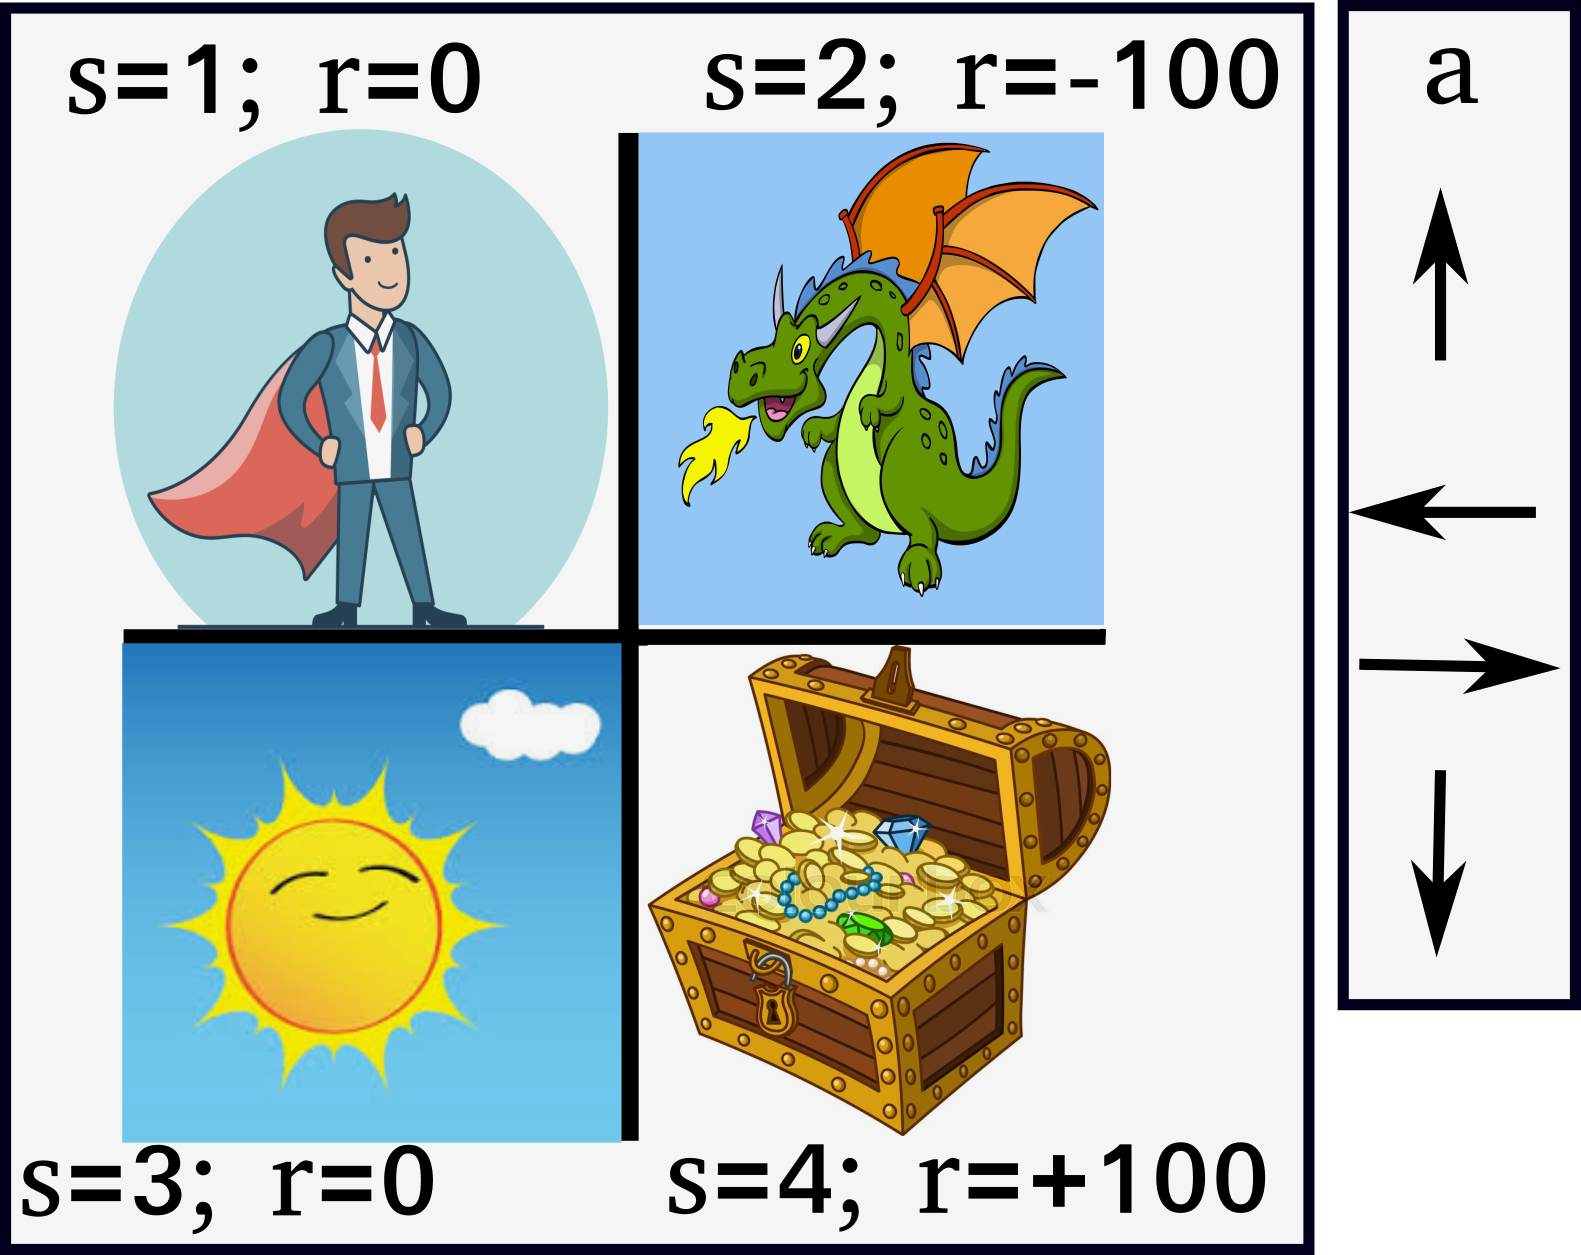
\includegraphics[width=0.35\textwidth]{./Figures/ANNs_reinforcement_learning/Q_learning_example}
    \end{center}

    What does $Q^{*}(s, a)$ look like? Now learn, use $\alpha = 0.1$, $\gamma = 0.5$, $\epsilon = 1$: d;r.

    \begin{center}
      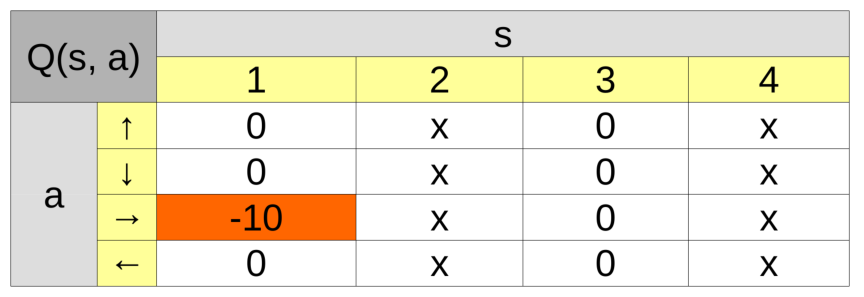
\includegraphics[width=0.46\textwidth]{./Figures/ANNs_reinforcement_learning/Q_learning_example_1}
      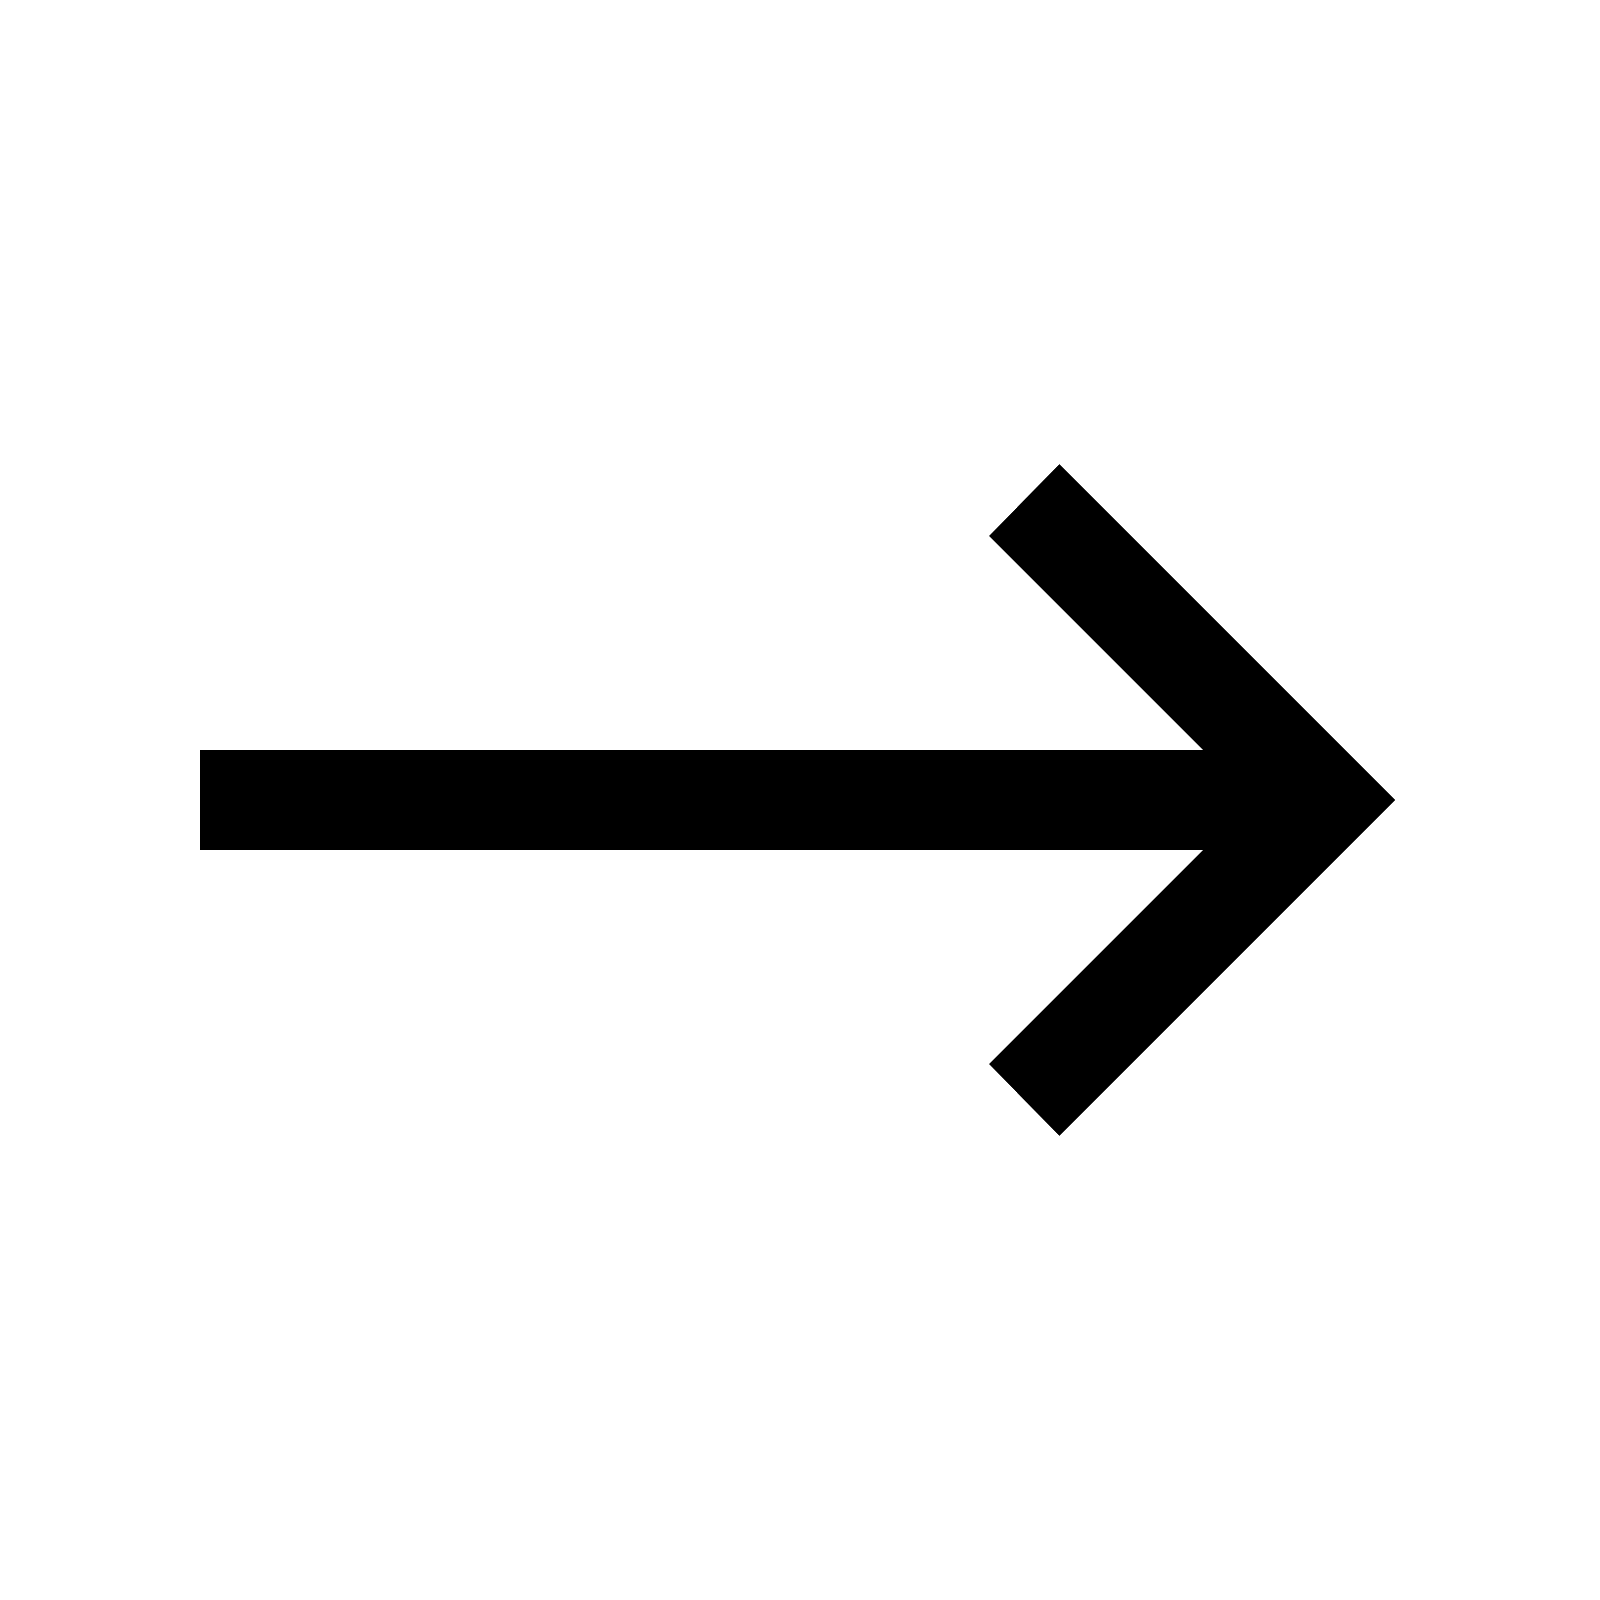
\includegraphics[width=0.05\textwidth]{./Figures/ANNs_reinforcement_learning/arrow_right}
      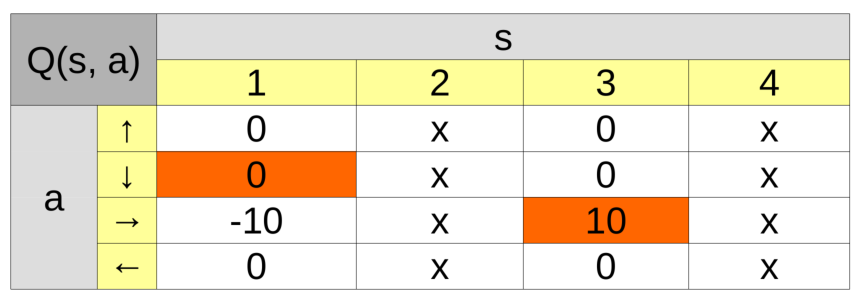
\includegraphics[width=0.46\textwidth]{./Figures/ANNs_reinforcement_learning/Q_learning_example_2}
    \end{center}
\end{frame}



\begin{frame}{Q-learning on an example}
    Simple example: a 2 x 2 matrix game.

    \begin{center}
      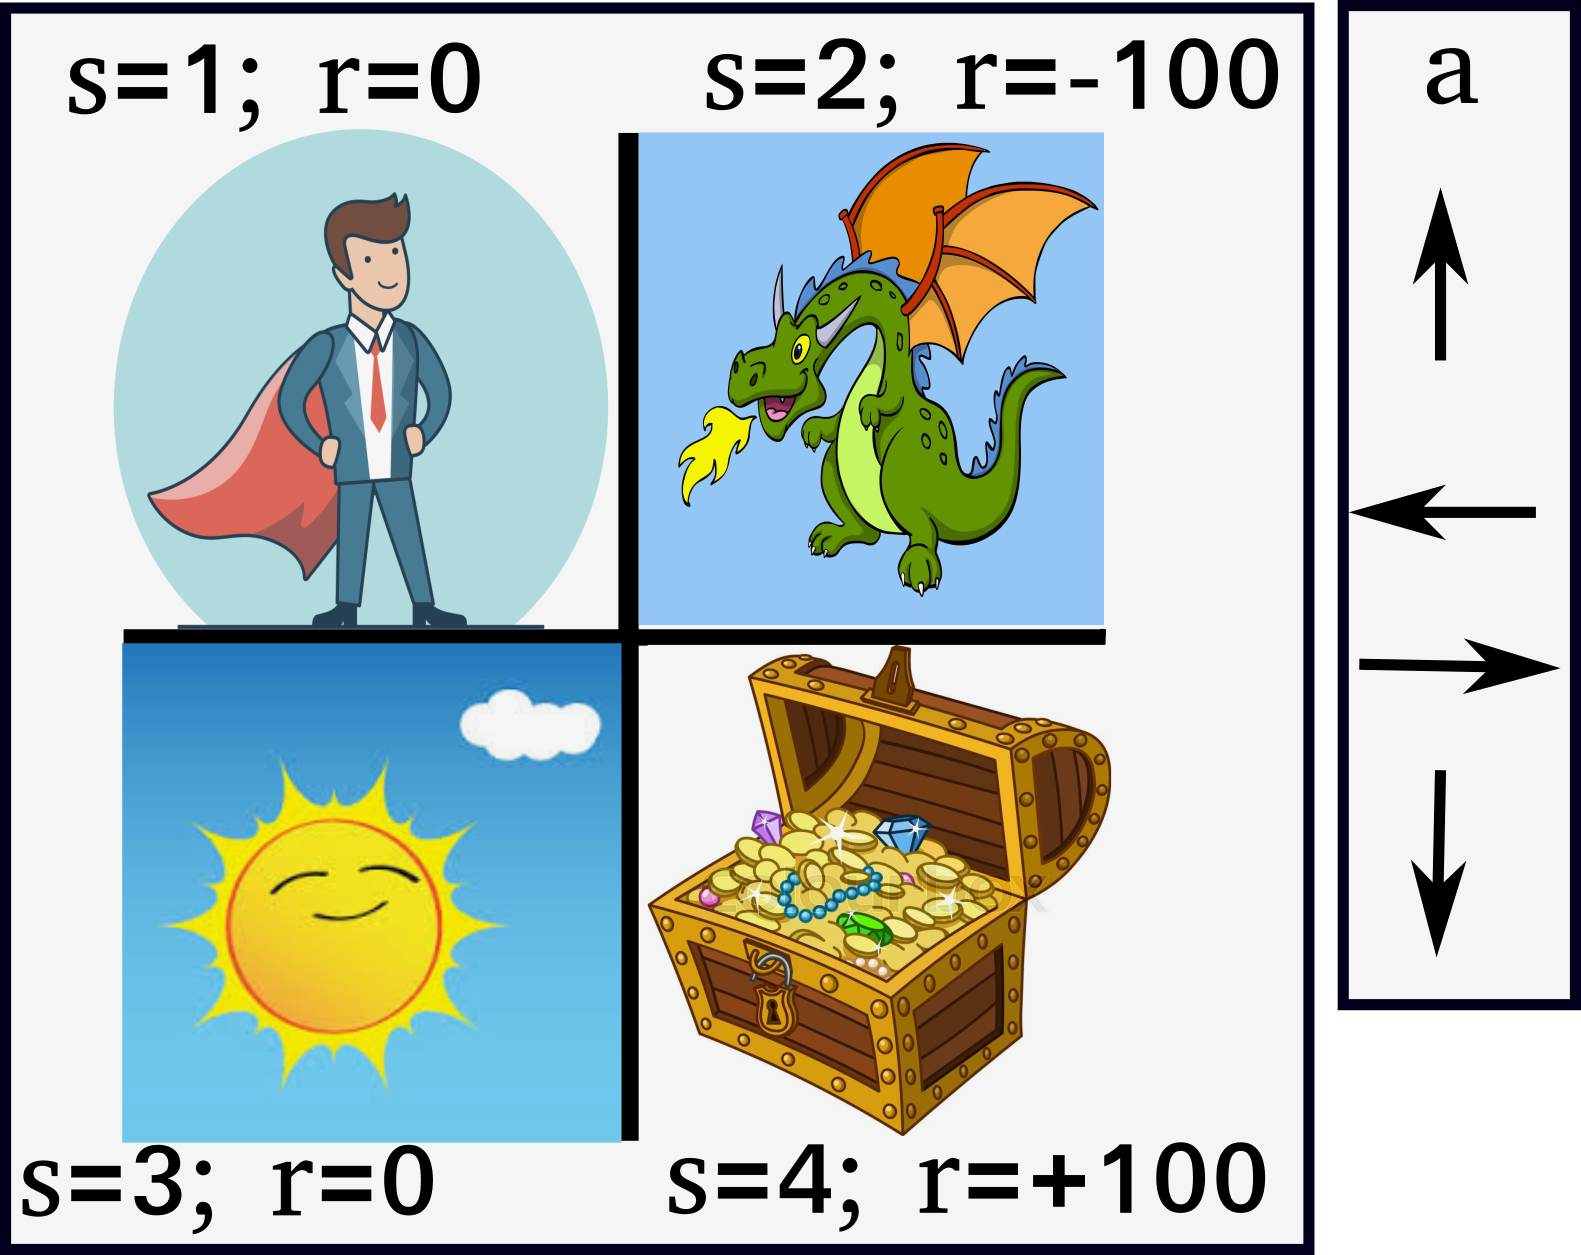
\includegraphics[width=0.35\textwidth]{./Figures/ANNs_reinforcement_learning/Q_learning_example}
    \end{center}

    What does $Q^{*}(s, a)$ look like? Now learn, use $\alpha = 0.1$, $\gamma = 0.5$, $\epsilon = 1$: d;u;d,r.

    \begin{center}
      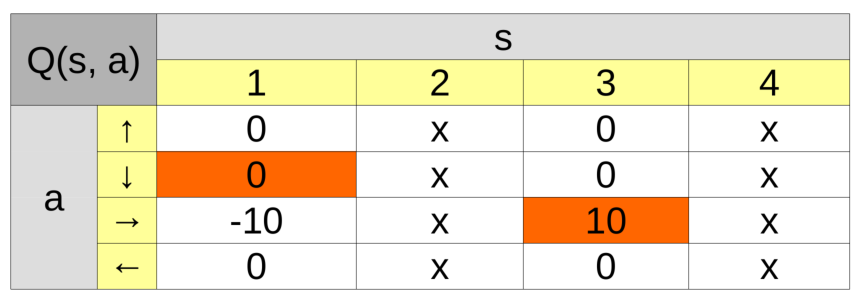
\includegraphics[width=0.46\textwidth]{./Figures/ANNs_reinforcement_learning/Q_learning_example_2}
      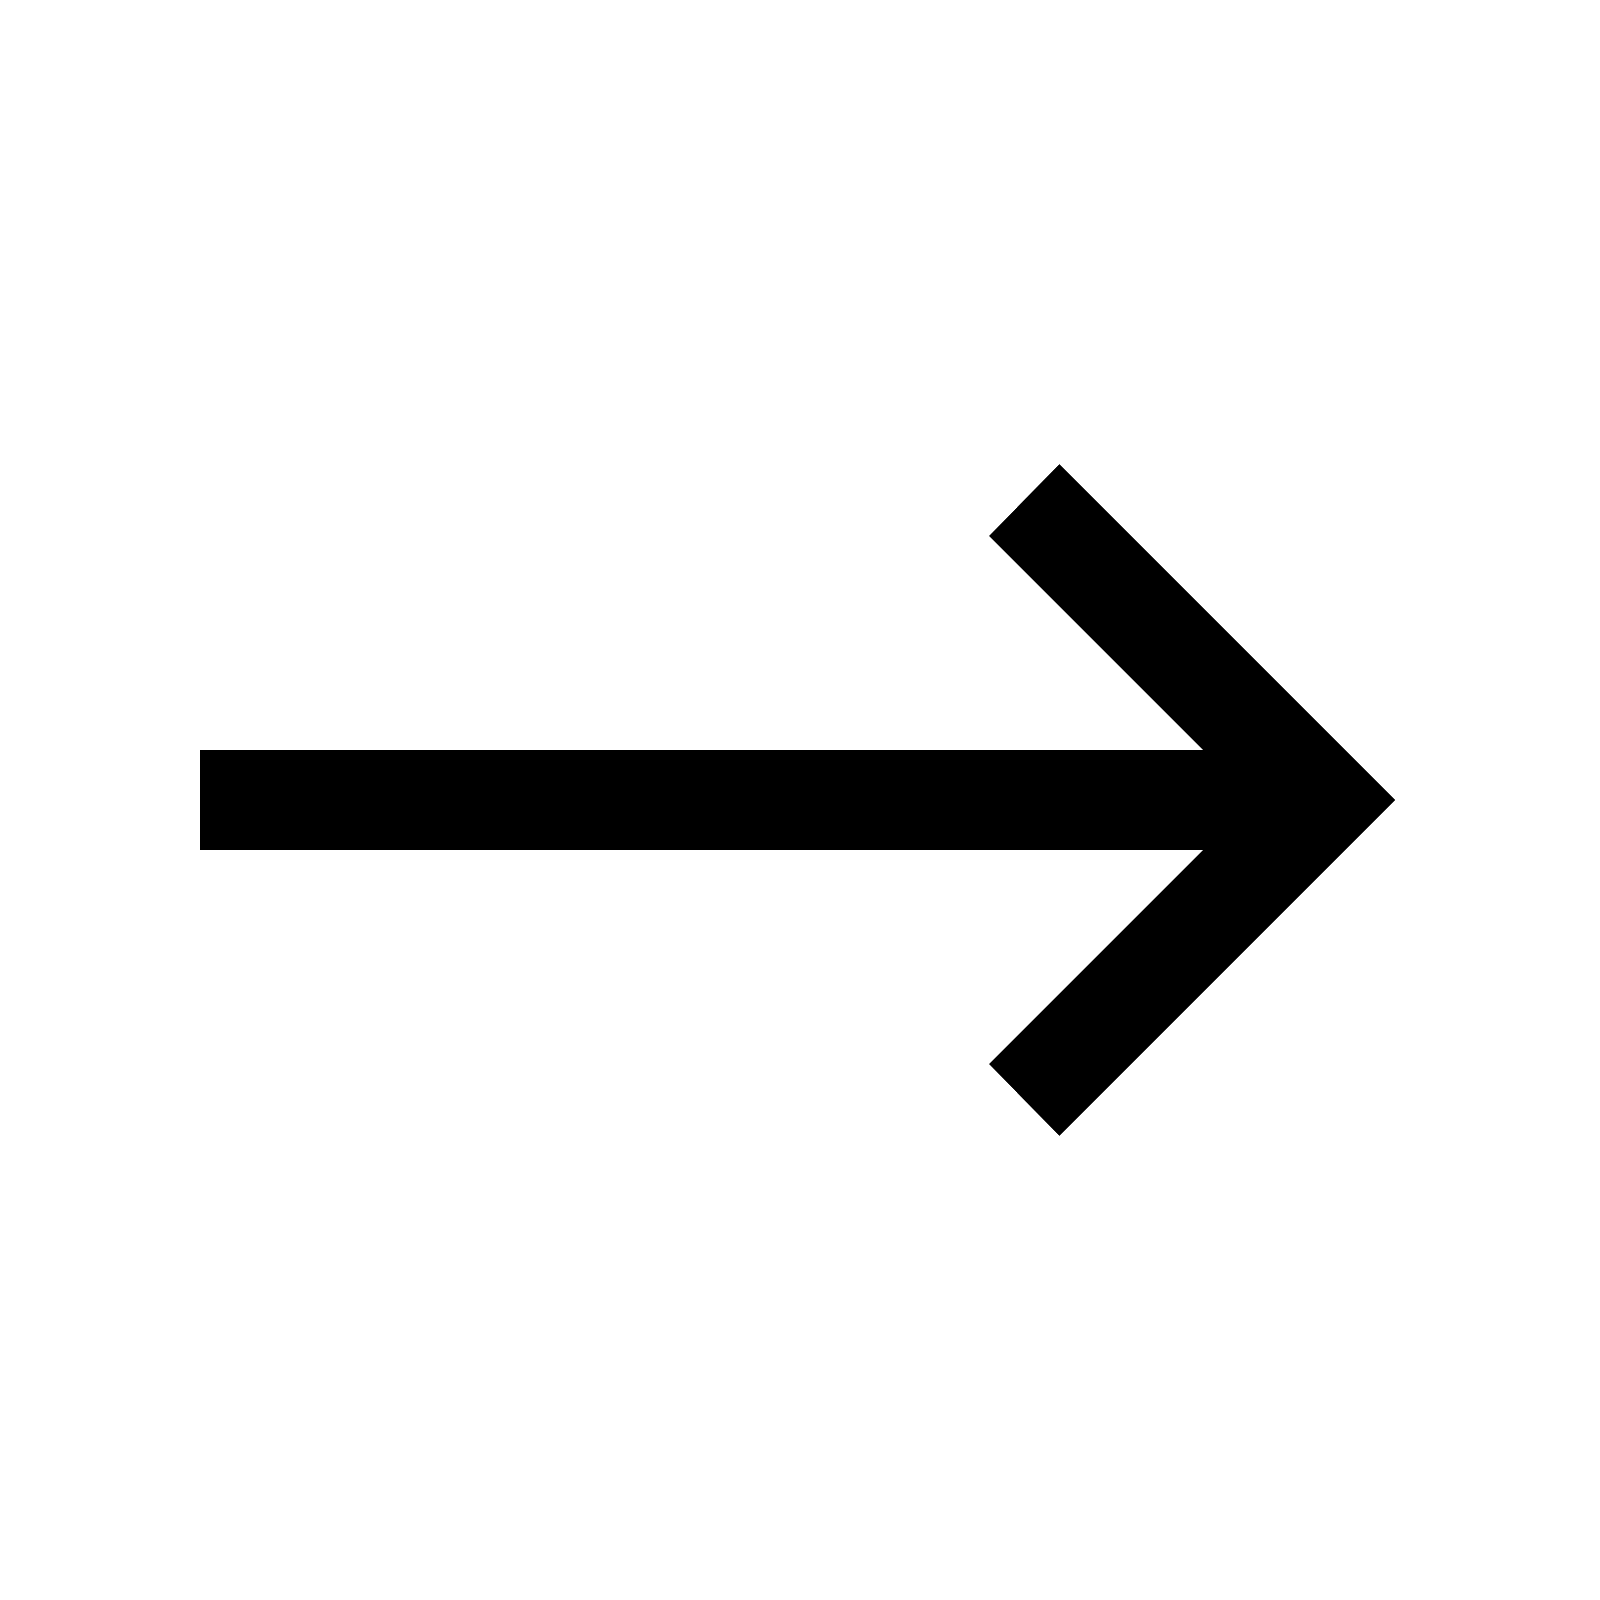
\includegraphics[width=0.05\textwidth]{./Figures/ANNs_reinforcement_learning/arrow_right}
      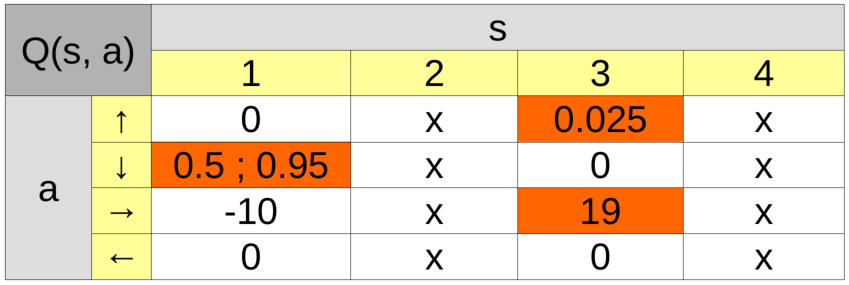
\includegraphics[width=0.46\textwidth]{./Figures/ANNs_reinforcement_learning/Q_learning_example_3}
    \end{center}
\end{frame}



\begin{frame}{Q-learning on an example}
    Simple example: a 2 x 2 matrix game.

    \begin{center}
      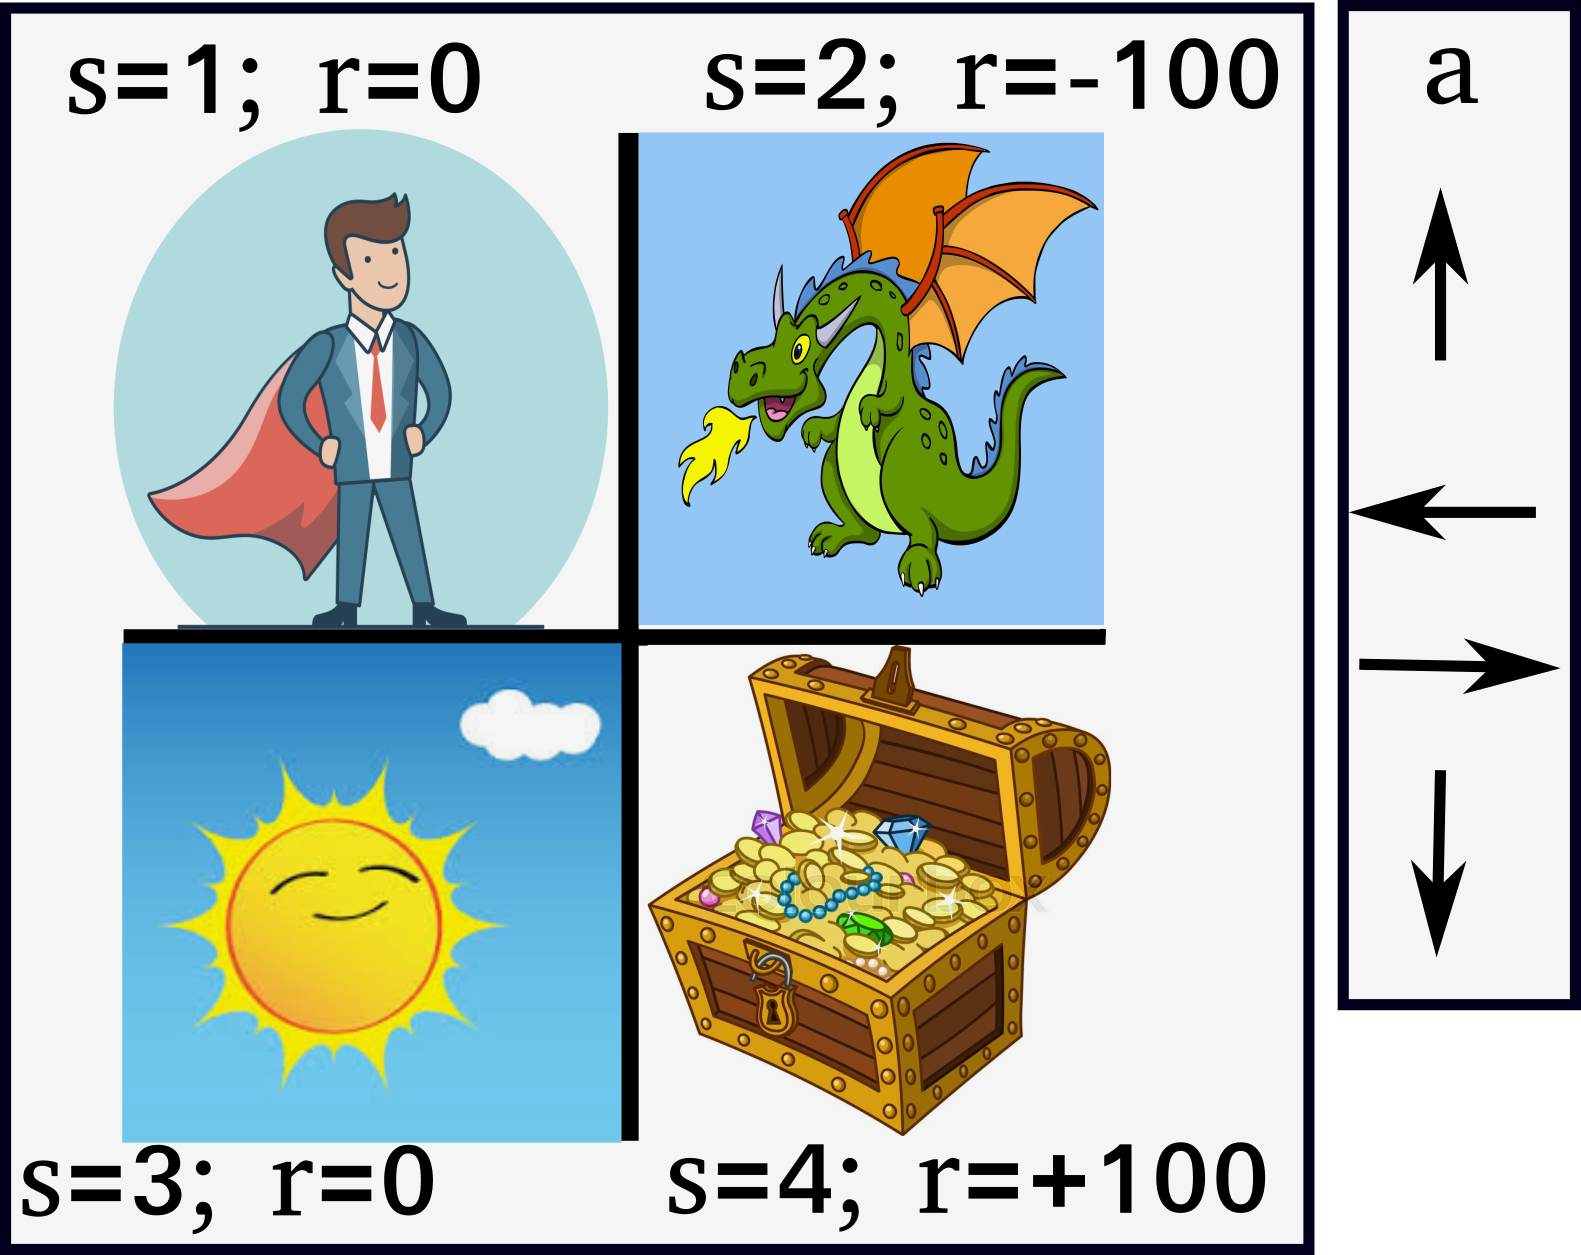
\includegraphics[width=0.35\textwidth]{./Figures/ANNs_reinforcement_learning/Q_learning_example}
    \end{center}

    What does $Q^{*}(s, a)$ look like? After many iterations, converge:

    \begin{center}
      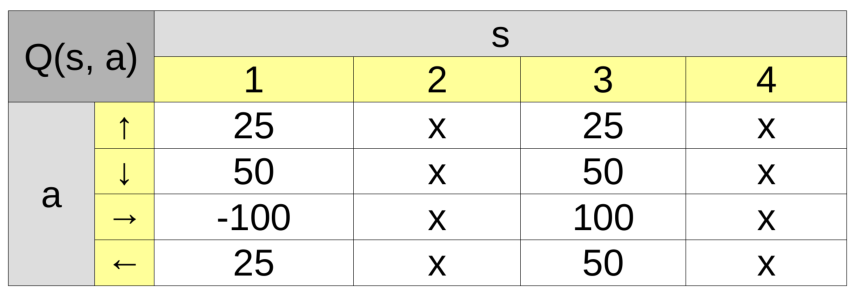
\includegraphics[width=0.7\textwidth]{./Figures/ANNs_reinforcement_learning/Q_learning_example_4}
    \end{center}
\end{frame}



\begin{frame}{The 'maze' illustration}
    Good way of thinking about Deep Q Learning: investigate a maze
    
    \begin{itemize}
        \item For each location, what is best possible output for each action.
        \item 'Good' probabilities diffuse.
    \end{itemize}
    
    \begin{center}
      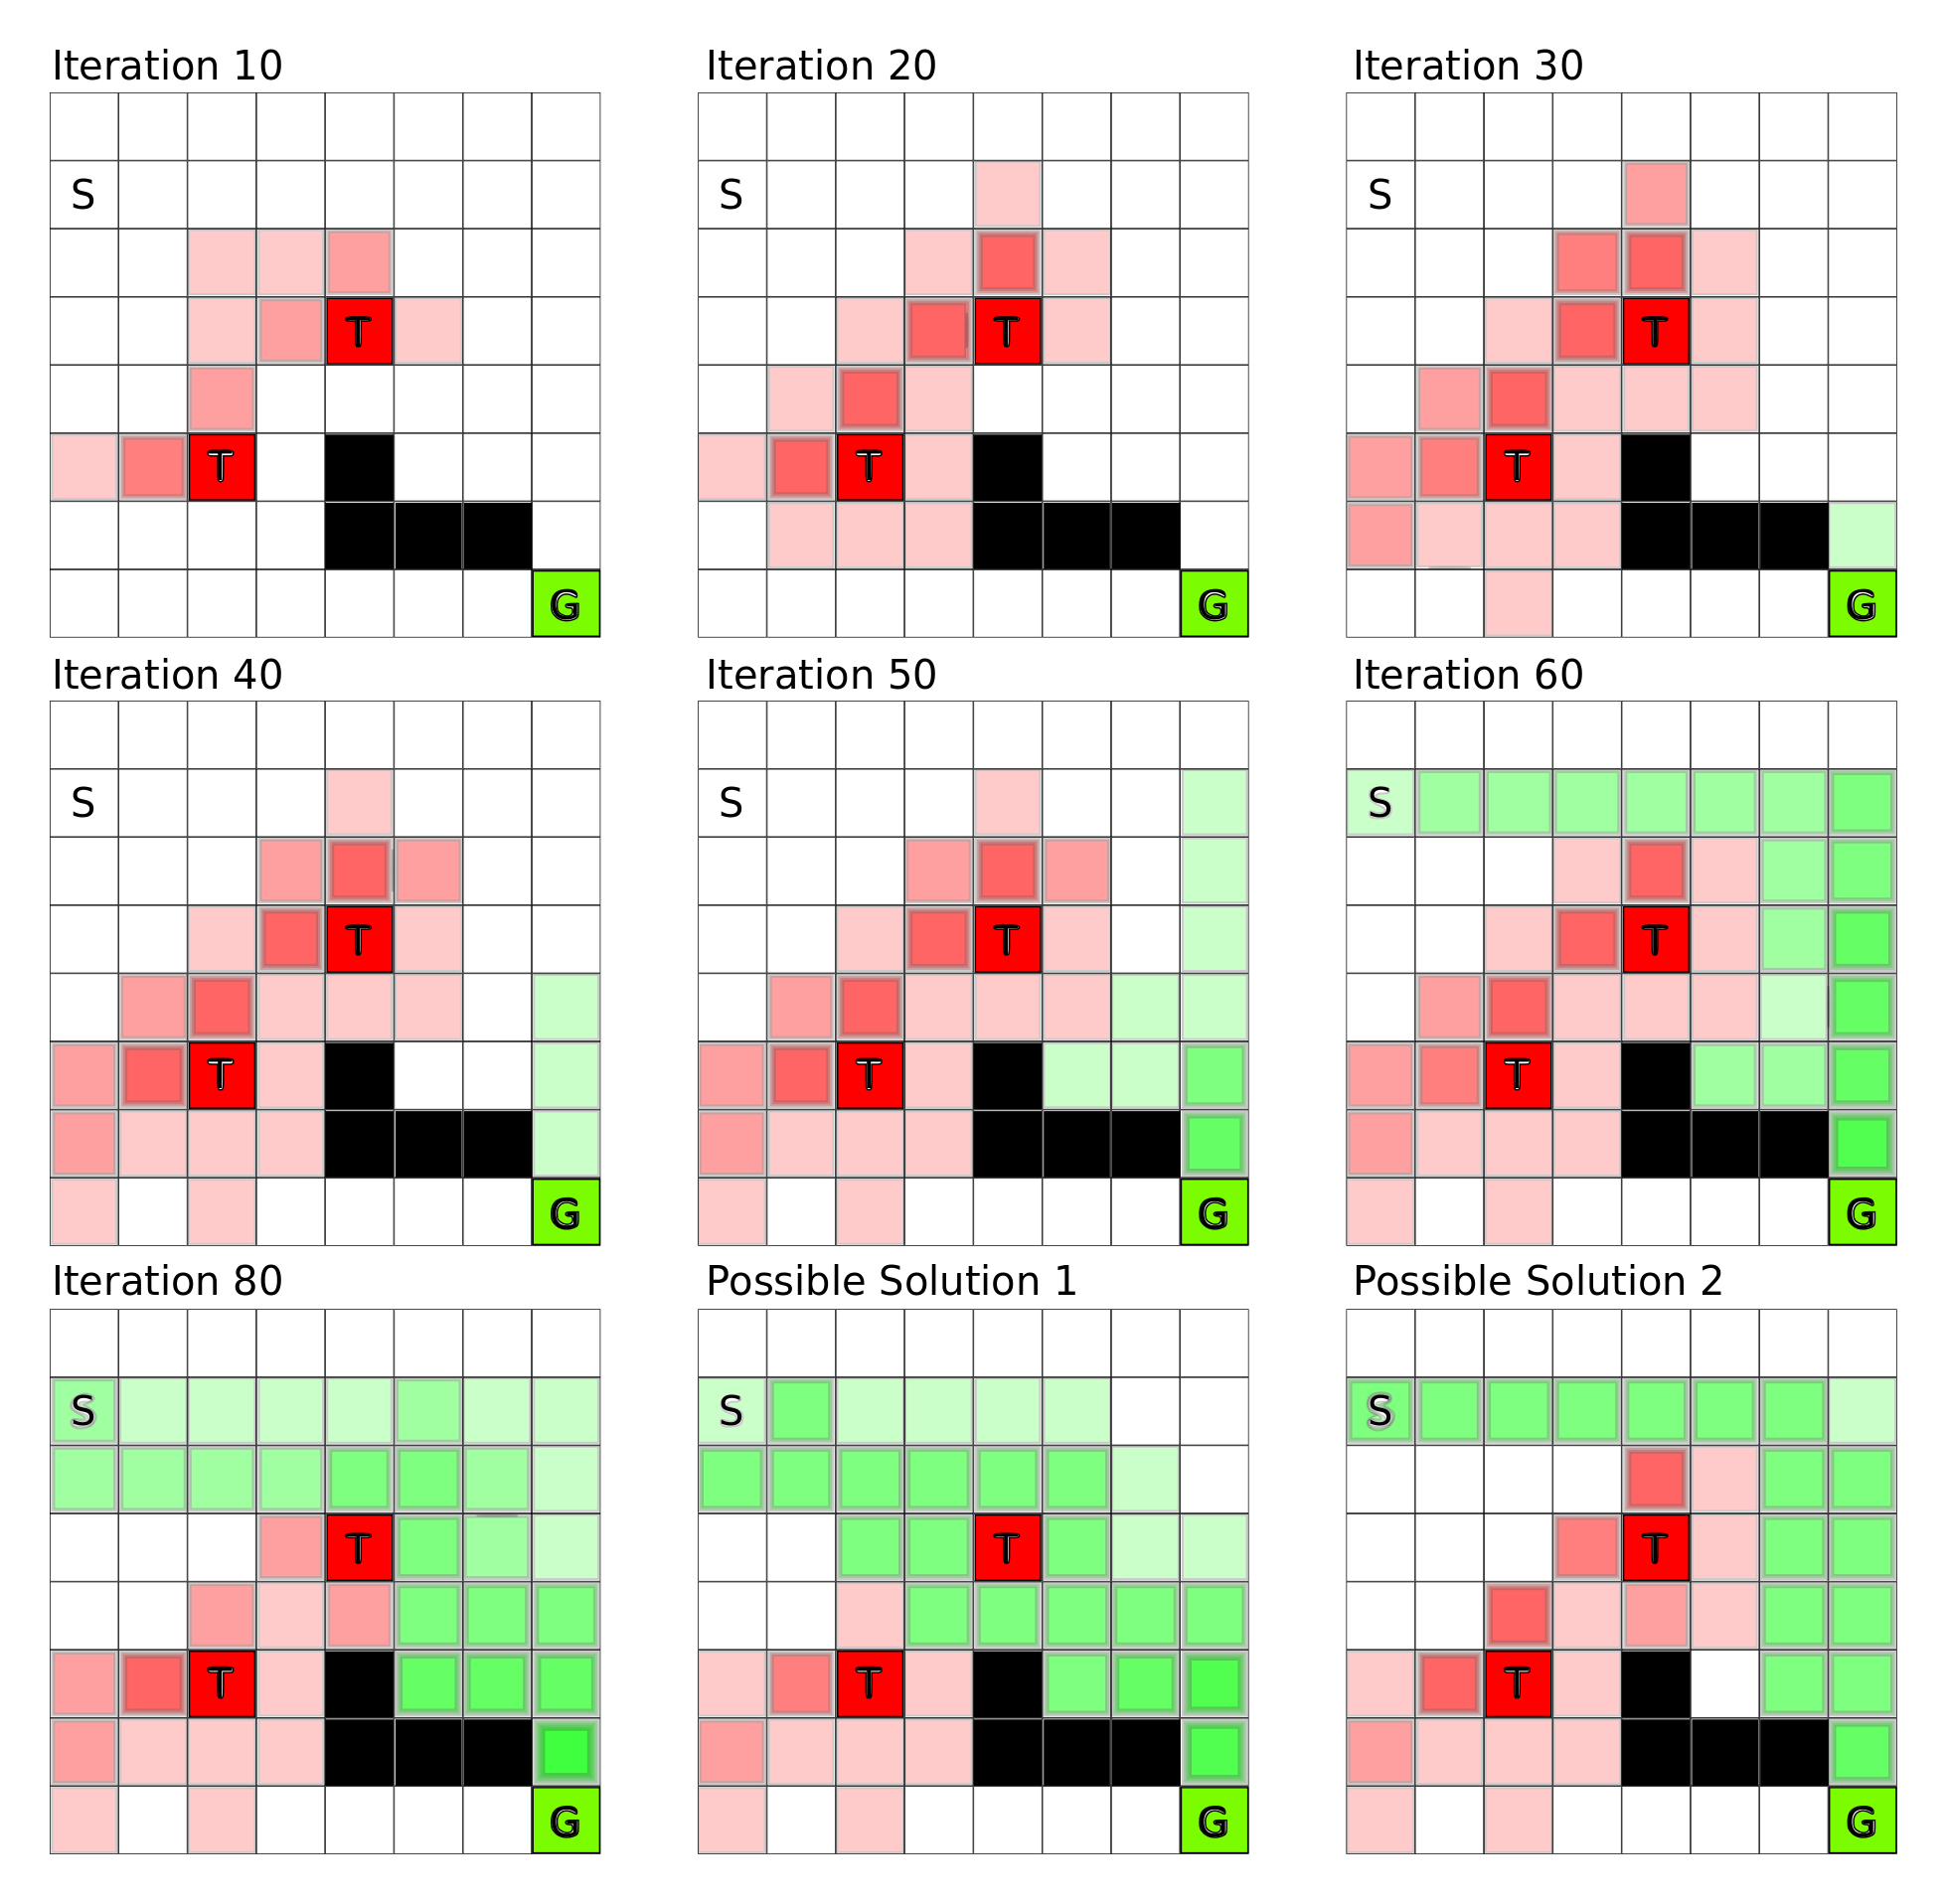
\includegraphics[width=0.5\textwidth]{./Figures/image_DQL}
    \end{center}
\end{frame}




\begin{frame}{Deep Q-Learning}
    World is non-linear, high dimensionality, complex...

    \begin{center}
      ... use a Deep Neural Network for $Q$. Therefore 'Deep Q-Learning'.
    \end{center}

    \begin{center}
      'Mastering the game of Go without human knowledge', \textit{Silver et. al.}, Nature (2015). \\
    \end{center}

    \begin{itemize}
      \item Parametrize $Q(s, a, \Theta_i)$ using a deep ANN ($\Theta_i$ network weights).
      \item max instead argmax: give the Q-value for each a in different output.
      \item Loss function: $L_i(\Theta_i) = \mathbb{E} \left[ \left( r + \gamma \max_{a'} Q(s', a', \Theta_i) - Q(s, a, \Theta_i) \right)^2 \right]$
      \item Experience replay buffer inspired from biology.
      \item Update target value at end of training for stability.
    \end{itemize}

   Computers that learn without us knowing a solution. Adapted to non-linear, high dimensional, complex problems. Can make DANNs fight each other (adversarial training). ANN just one solution (but works well).
\end{frame}

\section{ii. Policy Gradient method}

\begin{frame}{Policy Gradient methods}

\begin{center}
    Policy Gradient: directly learn the policy $\pi$.
  \end{center}

  Policy gradient vs Q-Learning:
  \begin{itemize}
    \item Often $\pi$ simpler than $Q$.
    \item $Q$: need to be able to effectively solve $\argmax$, tricky high dimension.
    \item Policy gradient: more versatile (continuous learning).
    \item $Q$: better exploration (can be taken care of).
  \end{itemize}
 
  Use a stochastic policy: $\pi$ is a distribution for each state input, parametrized by ANN:
  \begin{itemize}
    \item Smooths out actions.
    \item Train by slightly shifting distribution.
    \item ANN (weights $\Theta_i$) decides the parameters of a parametric distribution.
  \end{itemize}

  \begin{center}
    Objective: find $\Theta$ such that: $\max_{\Theta} \mathbb{E} \left[ \sum_{t=0}^{H} R(s_t) | \pi_{\theta} \right]$, $R(s_t) = r_t \gamma^t$
  \end{center}

\end{frame}


\begin{frame}{Computing the policy gradient}
  $\tau$: s-a sequence: ($s_0$, $a_0$), ($s_1$, $a_1$), ..., ($s_H$, $a_H$), $R(\tau) = \sum_{t=0}^{H}R(s_t, a_t)$ \\~\\

  \begin{center}
    Value: $V(\Theta) = \mathbb{E} \left[ \sum_{t=0}^{H} R(s_t, a_t) | \pi_{\theta} \right] = \sum_{\tau} \mathbb{P}(\tau, \Theta) R(\tau)$ \\
  \end{center}

  \begin{align*}
    \nabla_{\Theta} V(\Theta) &= \sum_{\tau} \nabla_{\Theta} \mathbb{P}(\tau, \Theta) R(\tau) \\
                              &= \sum_{\tau} \frac{\mathbb{P}(\tau, \Theta)}{\mathbb{P}(\tau, \Theta)} \nabla_{\Theta} \mathbb{P}(\tau, \Theta) R(\tau) \\
                              &= \sum_{\tau} \mathbb{P}(\tau, \Theta) \nabla_{\Theta} \log \left( \mathbb{P}(\tau, \Theta) \right) R(\tau)
  \end{align*}

  Expected value, approximate with empirical sampling under policy $\pi_{\theta}$:

  $$ \nabla_{\Theta} V(\Theta) \approx \hat{g} = \frac{1}{M} \sum_{i=1}^{M} \nabla_{\Theta} \log \left( \mathbb{P}(\tau^{(i)}, \Theta) \right) R(\tau^{(i)})$$
\end{frame}

\begin{frame}{Understanding the policy gradient}
  $$ \nabla_{\Theta} V(\Theta) \approx \hat{g} = \frac{1}{m} \sum_{i=1}^{M} \nabla_{\Theta} \log \left( \mathbb{P}(\tau^{(i)}, \Theta) \right) R(\tau^{(i)})$$

  \begin{itemize}
    \item Valid for discontinuous / unknown $R$.
    \item Works with discrete or continuous state / action. \\
  \end{itemize}

  Works by improving the probability of paths with good $R$ (and reducing the probability of paths with bad $R$).

  \begin{center}
    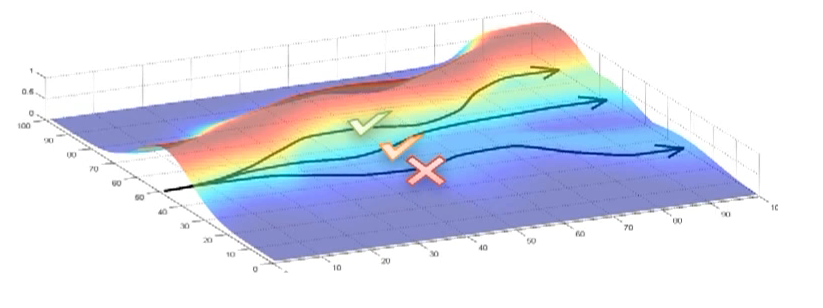
\includegraphics[width=0.58\textwidth]{Figures/illustration_policy_gradient}
  \end{center}
\end{frame}


\begin{frame}{Computing the gradient of the log probability}
  Express the log prob as a dynamics model and a policy part:
  \begin{align*}
    \nabla_{\Theta} \log \left( \mathbb{P}(\tau^{(i)}, \Theta) \right) &= \nabla_{\Theta} \log \left[ \prod_{t=0}^{H} \mathbb{P}(s_{t+1}^{(i)} | s_{t}^{(i)}, a_t^{(i)}) \pi_{\tau}(a_t^{(i)} | s_{t}^{(i)})  \right] \\
                                                                       &= \nabla_{\Theta} \left[ \sum_{t=0}^{H} \log \mathbb{P}(s_{t+1}^{(i)} | s_{t}^{(i)}, a_t^{(i)}) + \sum_{t=0}^{H} \log \pi_{\tau}(a_t^{(i)} | s_{t}^{(i)})  \right] \\
                                                                       &= \nabla_{\Theta} \sum_{t=0}^{H} \log \pi_{\tau}(a_t^{(i)} | s_{t}^{(i)})
  \end{align*}

  The log prob gradient depends only on the policy. No dynamics model. This method is unbiased:

    $$\nabla_{\Theta} V(\Theta) = \mathbb{E} \left[ \hat{g} \right],$$

  so use $ \nabla_{\Theta} V(\Theta) \approx \hat{g} = \frac{1}{m} \sum_{i=1}^{M} \nabla_{\Theta} \log \left( \mathbb{P}(\tau^{(i)}, \Theta) \right) R(\tau^{(i)})$, \\
  with $\nabla_{\Theta} \log \left( \mathbb{P}(\tau^{(i)}, \Theta) \right) = \nabla_{\Theta} \sum_{t=0}^{H} \log \pi_{\tau}(a_t^{(i)} | s_{t}^{(i)})$.

\end{frame}

\begin{frame}{Importance sampling and off-policy learning}
Derivations so far are 'on-policy':

\begin{itemize}
  \item Use same policy to explore (i.e. collect samples) and compute the policy gradient.
  \item Poor sampling efficiency: need new samples each time policy is updated.
\end{itemize}

Unrealistic in reality. Resort to \textbf{importance sampling}: 

\begin{center}
  Use old samples, but compensate for distribution shifts.
\end{center}

This allows to study one distribution, while sampling from another one.

\begin{align*}
  \mu &= \mathbb{E}_p(f) = \int_D f(x) p(x) dx \\
      &= \int_D \frac{f(x) p(x)}{q(x)} q(x) dx = \mathbb{E}_q \left( \frac{f(X)p(X)}{q(X)} \right)
\end{align*}

\end{frame}




\begin{frame}{Surrogate objective and KL norm penalization}
Re-write value function:
\begin{align*}
    V(\theta) &= \sum_t \mathbb{E}_{(s_t, a_t) \sim p_{\theta}(s_t, a_t)} [r_t(s_t, a_t) \gamma^t] \\
              &= \sum_t \mathbb{E}_{s_t \sim p_\theta(s_t)} [\mathbb{E}_{a_t \sim \pi_\theta(a_t | s_t)} [r_t(s_t, a_t) \gamma^t]]
\end{align*}    

    so that applying importance sampling:
    
$$ V(\theta') = \sum_t \mathbb{E}_{s_t \sim p_\theta(s_t)} \left[ \frac{p_{\theta'}(s_t)}{p_\theta(s_t)}  \mathbb{E}_{a_t \sim \pi_\theta(a_t | s_t)} \left[ \frac{\pi_{\theta'}(a_t | s_t)}{\pi_\theta(a_t | s_t)} r_t(s_t, a_t) \gamma^t \right] \right] $$
    
    Therefore to allow re-use of previous trajectories:
    
\begin{itemize}
  \item Optimize (advantage) surrogate objective: $\underset{\theta}{max} \left( \mathbb{E}  \left[ \frac{\pi_\theta (a_t \vert s_t)}{\pi_{\theta_{old}} (a_t \vert s_t)} \hat{A_t} \right] \right) $
  \item With constraint: $ \mathbb{E} \left[ KL( \pi_{\theta_{old}}( \cdot | s_t), \pi_{\theta}( \cdot | s_t)) \right] < \delta $
\end{itemize}

KL = Kullback Leibler divergence ('difference' between 2 distributions).
    
\end{frame}


\begin{frame}{Many refinements...}

Many more refinements than we have time for today.

Read:

\begin{itemize}
    \item "Advanced Policy Gradient Methods", Joshua Achiam: \url{http://rail.eecs.berkeley.edu/deeprlcourse-fa17/f17docs/lecture_13_advanced_pg.pdf} .
    \item "Proximal Policy Optimization Algorithms", John Schulman et. al., ArXiv (2017), \url{https://arxiv.org/pdf/1707.06347.pdf} .
\end{itemize}

\end{frame}




\begin{frame}{Training vs. deterministic runner}
    Training:
    
    \begin{itemize}
        \item Generate pdf of action following current ANN policy.
        \item Randomly sample from the distribution
    \end{itemize}
    
    Therefore, perform exploration, and do not follow the policy believed to be optimal. Visible as exploration
    noise in control strategy. \\~\\
    
    Deterministic runner:
    
    \begin{itemize}
        \item Idem: generate pdf of action following trained ANN policy.
        \item Pick as action the one 'most likely' to be optimal, i.e. maximum of the distribution.
    \end{itemize}
    
    Can provide smooth policy.
\end{frame}


\begin{frame}{Proximal Policy Optimization (PPO)}
     State of the art gradient based method:
    
    \begin{center}
      'Proximal Policy Optimization Algorithms', \textit{Schulman et. al.}, ArXiv (2017). \\
    \end{center}

    Implement a few tricks:

    \begin{itemize}
        \item Critic network: learn (noisy) actualized reward with a separate ANN.
        \item Clip gradient (instead of use KL) to discourage unsafe policy changes.    
    \end{itemize}
    
    Used in the following; Open Source implementation:
    
    \begin{center}
      'Tensorforce: a TensorFlow library for applied reinforcement learning', \textit{Kuhnle et. al.}, Github (2017) \\
      \textit{https://github.com/tensorforce/tensorforce}
    \end{center}
    
    Built as a Tensorflow computational graph for efficiency.
\end{frame}

\begin{frame}{Real world application}
    Video games; Go; Poker, Rubik's cube; some recent industry deployments:
    
    \begin{center}
        ''Google just gave control over data center cooling to an AI'', \\ \textit{MIT Technology Review}, Aug. 2018.
    \end{center}

    Energy saving in servers cooling, -40\% cooling electricity use.

    \begin{center}
    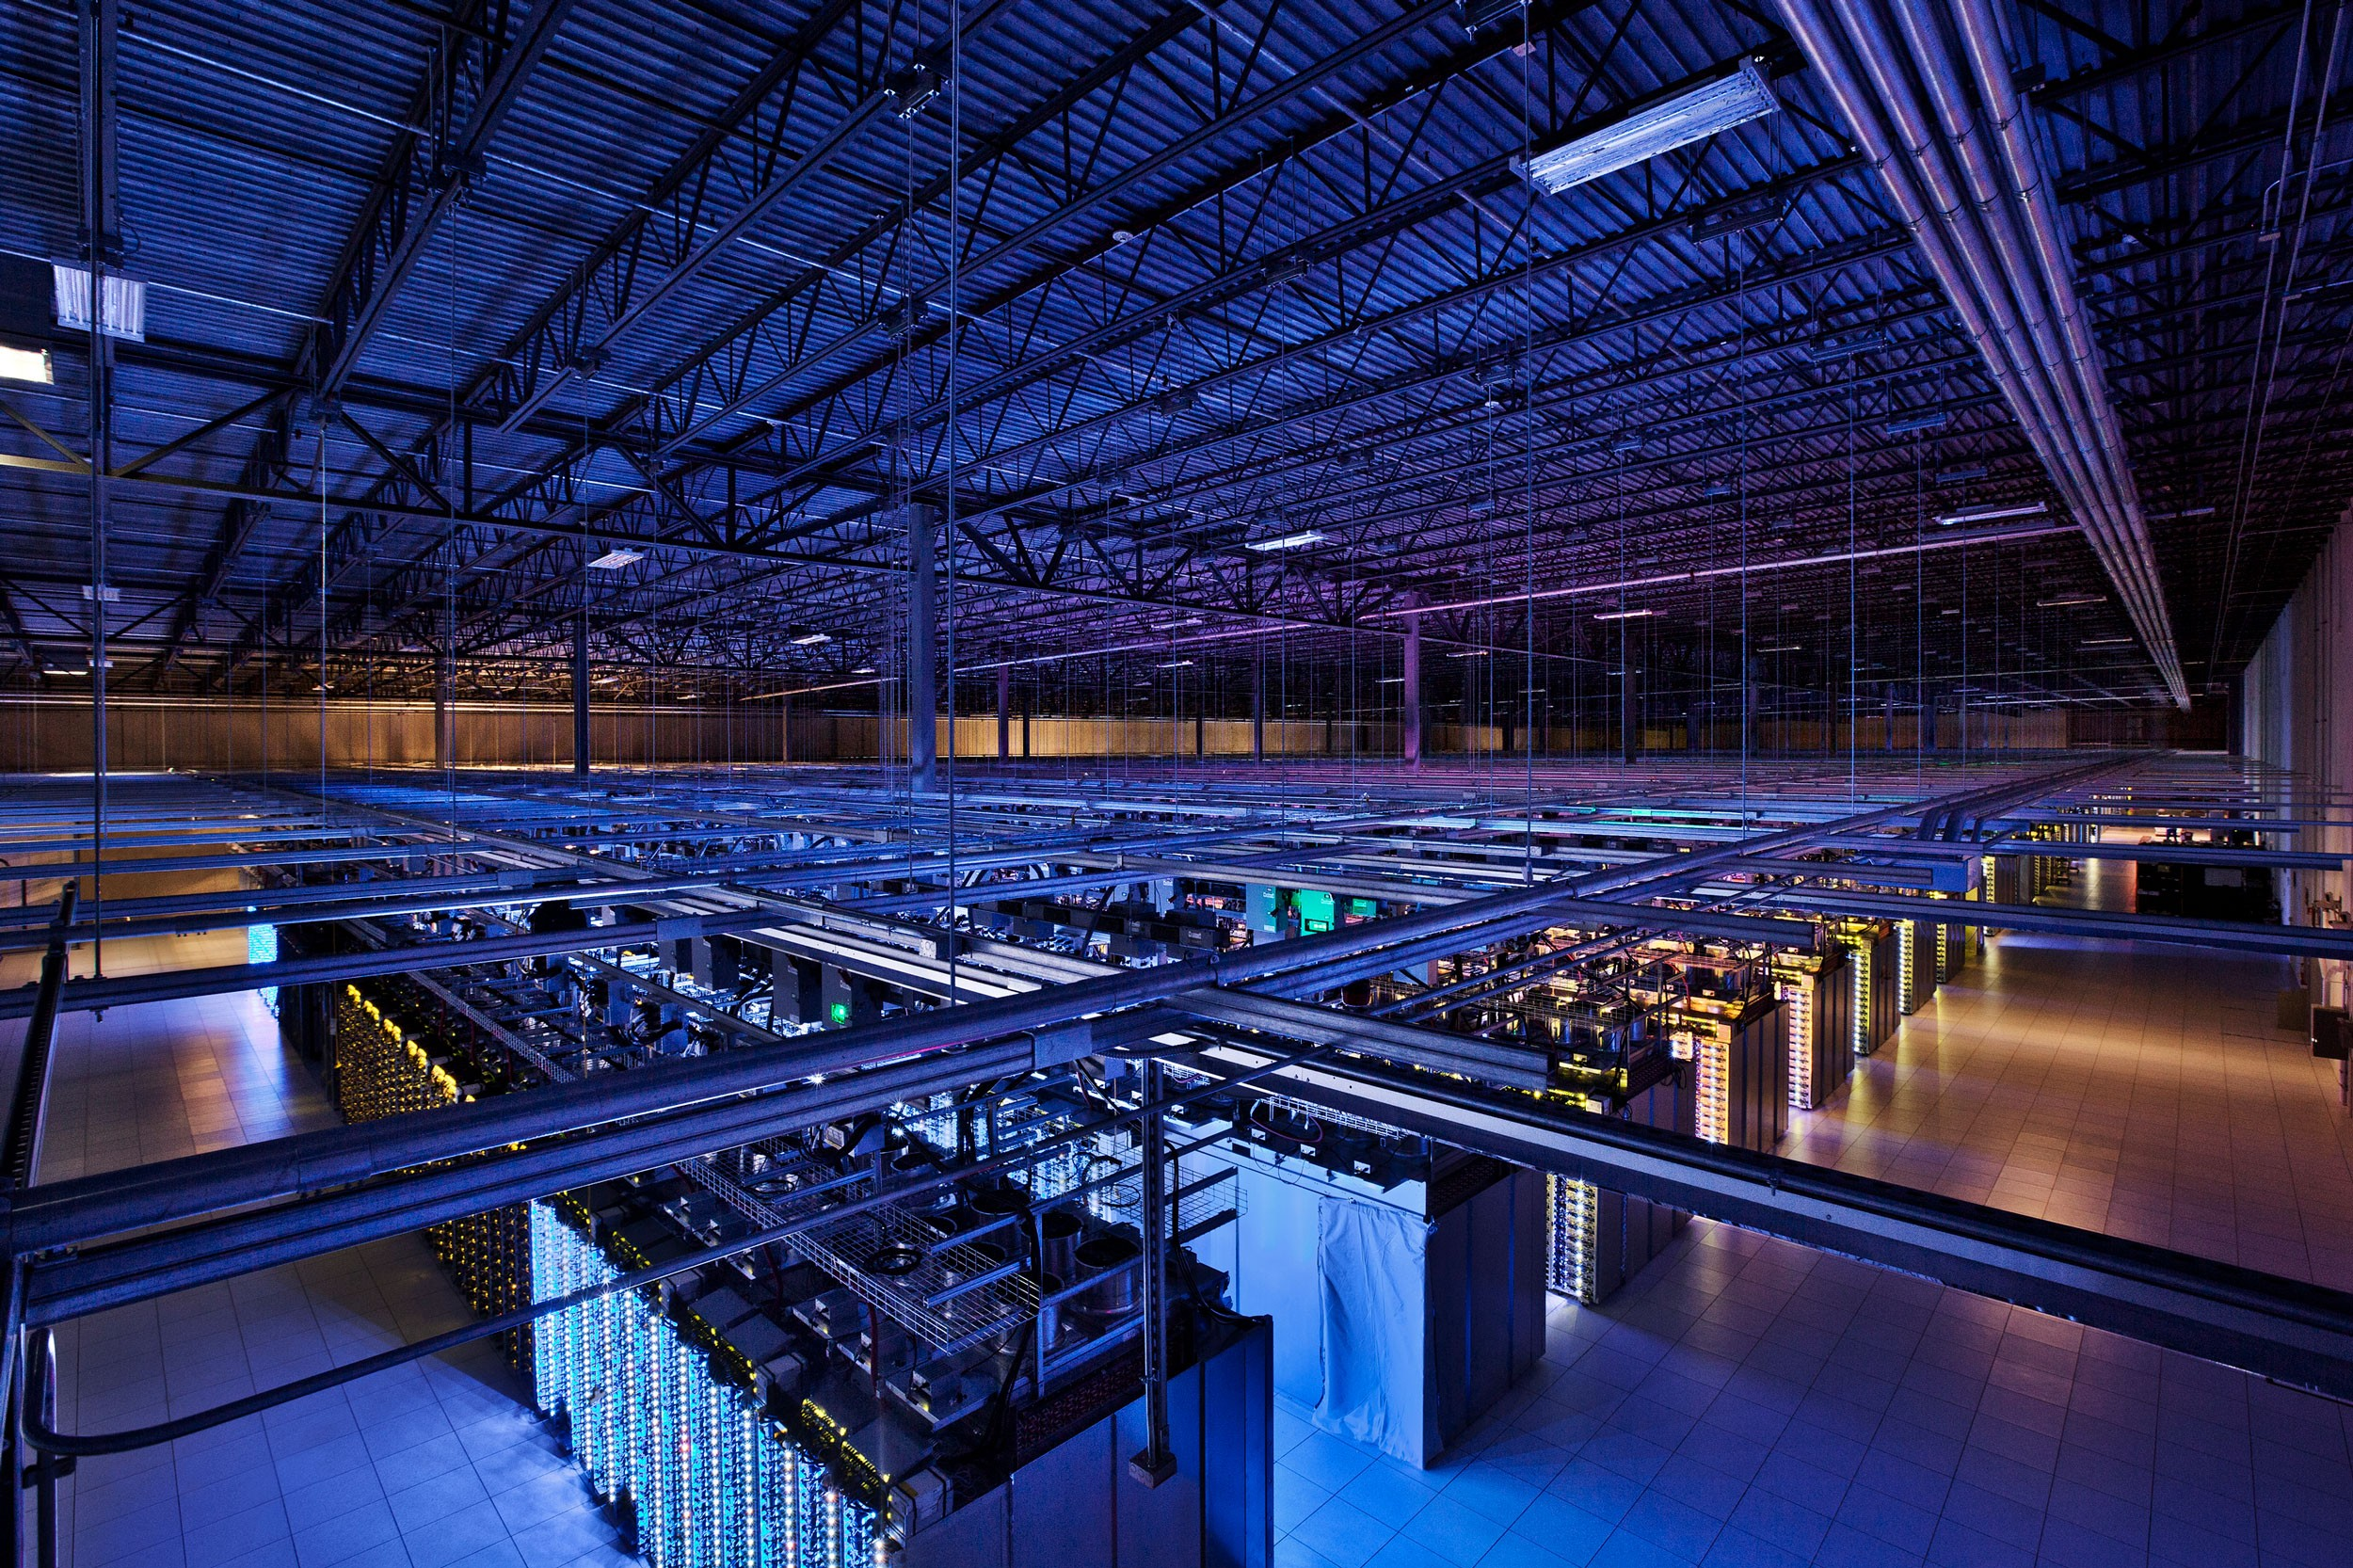
\includegraphics[width=0.58\textwidth]{Figures/servers}
    \end{center}
\end{frame}


\begin{frame}{A nice video illustration of DRL effectiveness}
    
    \begin{center}
    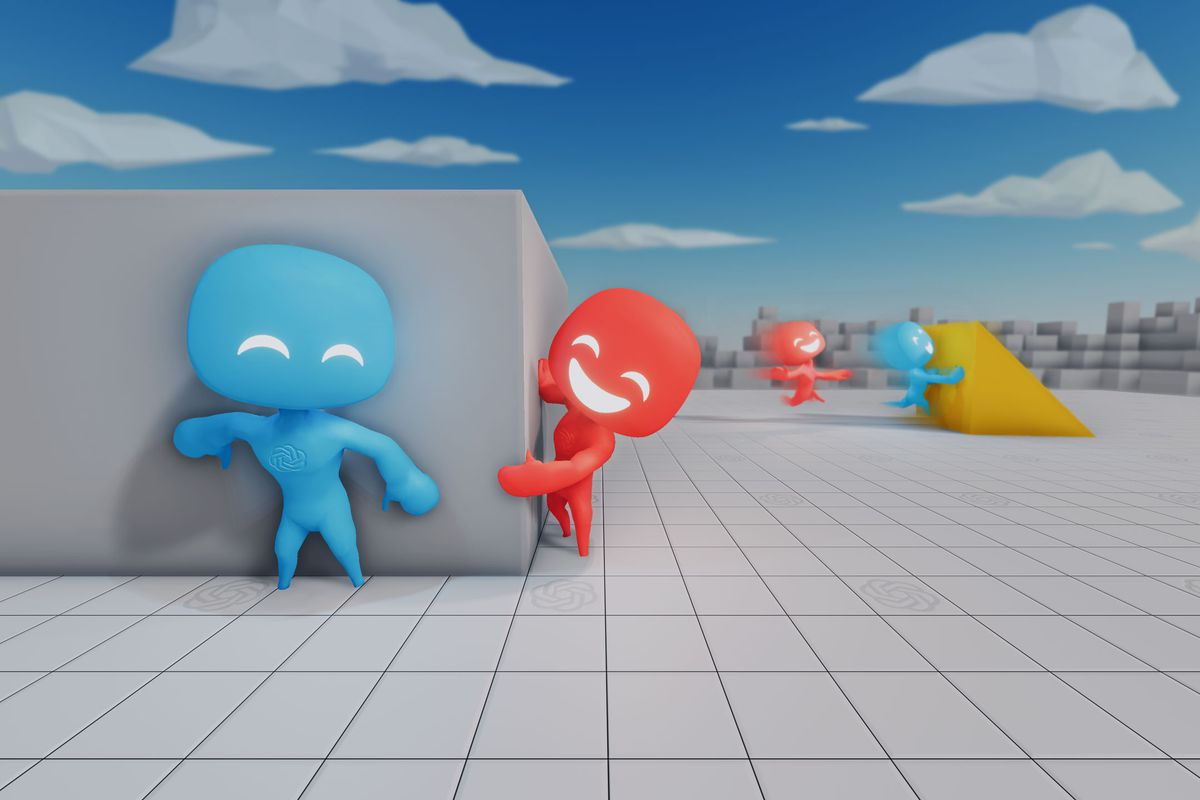
\includegraphics[width=0.70\textwidth]{Figures/hideandseek}
    \end{center}

    \begin{center}
      https://youtu.be/kopoLzvh5jY
    \end{center}
\end{frame}


\section{iii. Refinements and amelioration of RL algorithms}

\begin{frame}{World models}
"World Models", Ha and Schmidhuber, ArXiv / NIPS (2018).
 
    \begin{itemize}
        \item Learn the control and the model at the same time.
        \item Supervised learning of the model.
        \item Use it for training without the env.
        \item May use the same ANN to enrich output.
    \end{itemize}

    \begin{center}
    'Getting ANNs to dream'
    \end{center}

    \begin{center}
    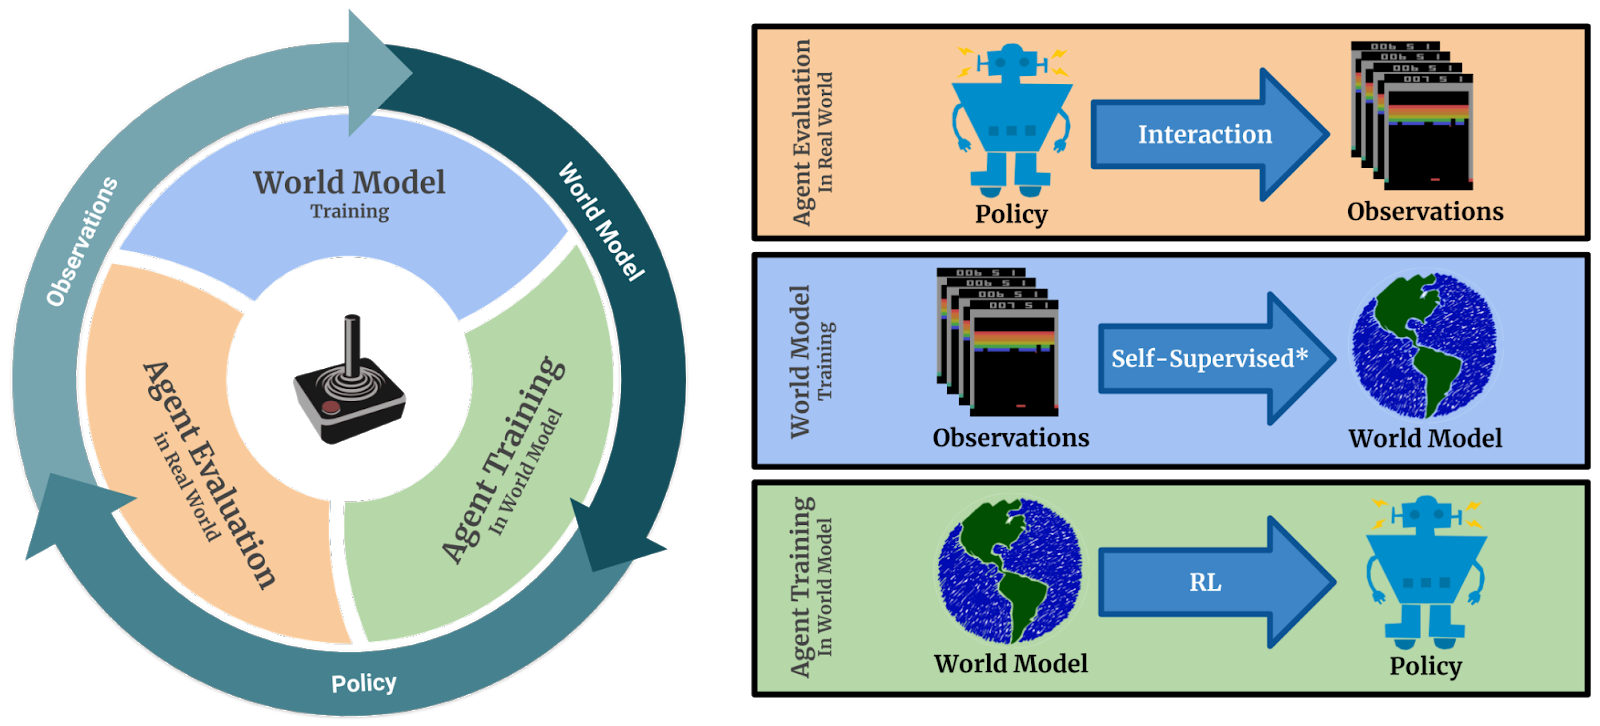
\includegraphics[width=0.70\textwidth]{Figures/world_model}
    \end{center}

\end{frame}

\begin{frame}{Curiosity}
"Surprise-Based Intrinsic Motivation for Deep Reinforcement Learning", J. Achiam, S. Sastry, ArXiv (2017).

    \begin{itemize}
        \item How to favorize exploration?
        \item How to make sure ANN explores the whole system?
    \end{itemize}

    \begin{center}
        reward = (env reward) + (surprise reward)
    \end{center}

    Surprise reward:
\begin{itemize}
    \item The ANN also tries to predict next state.
    \item Reward based on how different next state vs. prediction.
\end{itemize}

    \begin{center}
    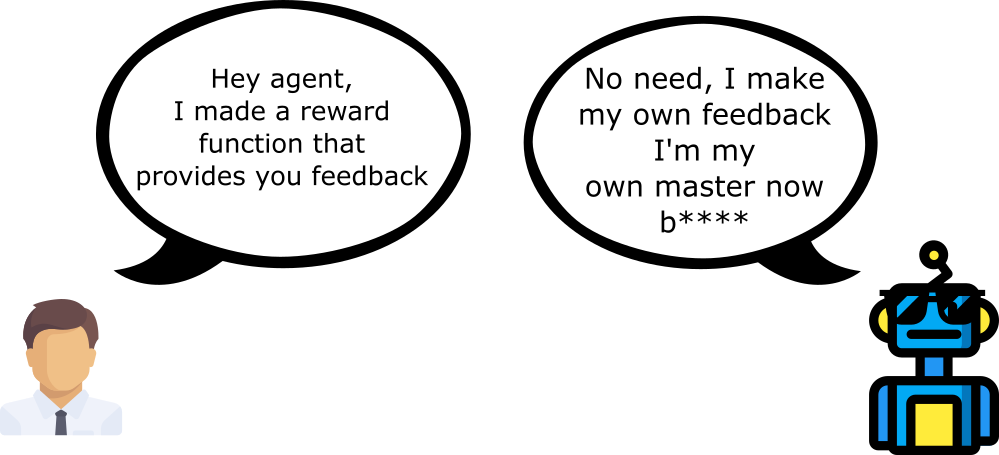
\includegraphics[width=0.70\textwidth]{Figures/curiosity}
    \end{center}

\end{frame}

\begin{frame}{Curiosity through reachability}
"Episodic Curiosity through Reachability", N. Savinov et. al., ArXiv (2018). \\~\\

    Problem of vanilla curiosity-driven:
    \begin{itemize}
        \item Procrastination.
        \item 'couch potato' in front of random TV.
    \end{itemize}

    \begin{center}
        Base 'surprise reward' on distance in terms of number of actions.
    \end{center}

    \begin{center}
    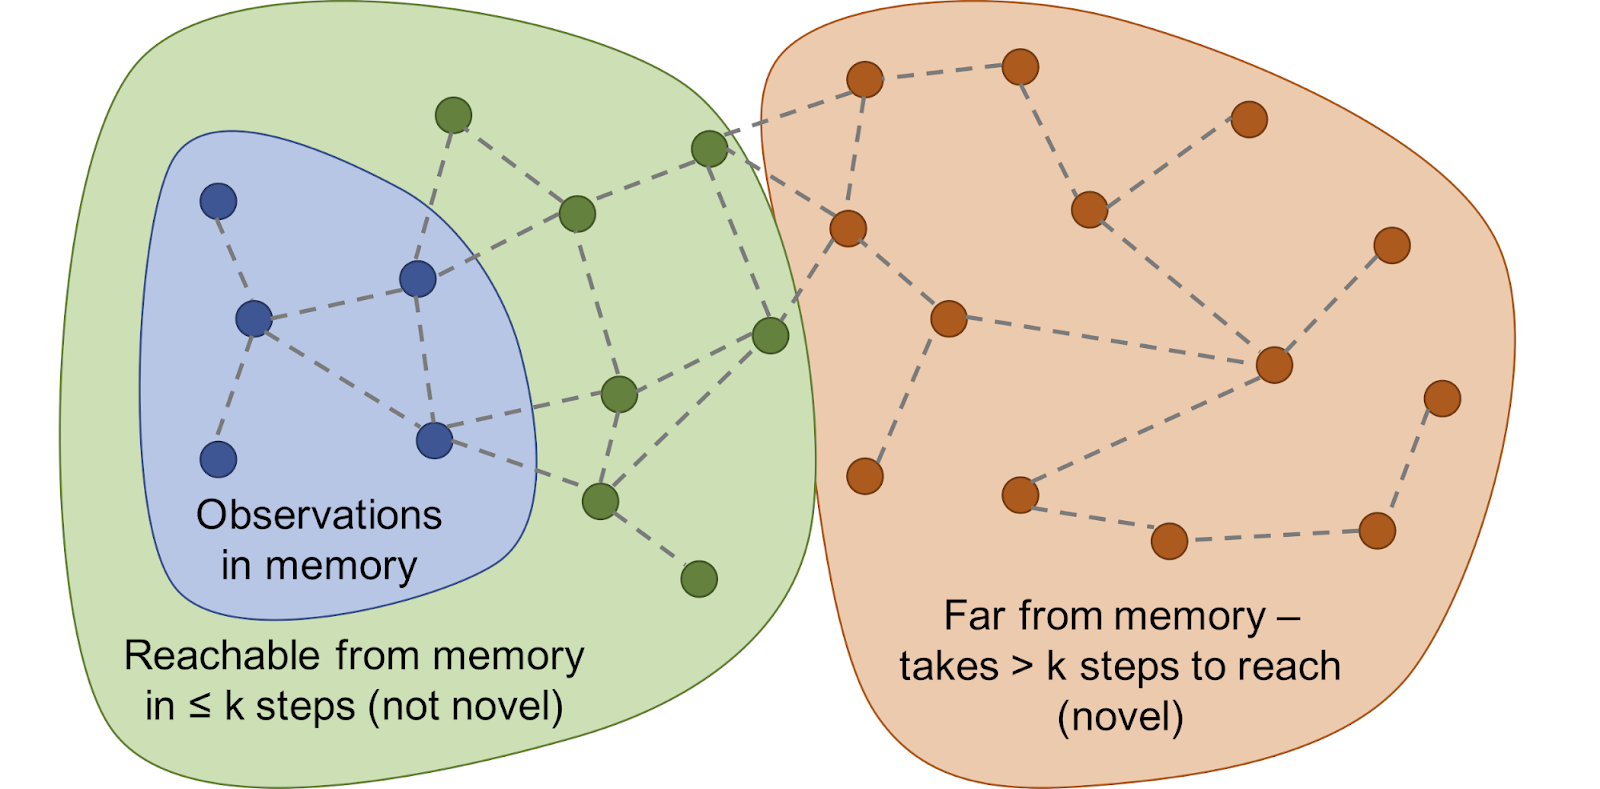
\includegraphics[width=0.70\textwidth]{Figures/curiosity_reachability}
    \end{center}
\end{frame}

\begin{frame}{Teaching through example}
"Learning Montezuma's Revenge from a Single Demonstration",  Tim Salimans and Richard Chen , OpenAI blog (2018). \\~\\

    Huge cost in exploration:
    \begin{itemize}
        \item Take a game when need to perform exact sequence of actions.
        \item Exploration cost exponential in sequence length.
        \item The 'Moteczuma revenge' benchmark.
        \item DRL has difficulty with long chains of causal actions and sparse reward.
    \end{itemize}

    Solution:
    \begin{itemize}
        \item Provide some example games.
        \item Start at random position in the example.
    \end{itemize}

    Drastically cut the cost of exploration.
\end{frame}

\begin{frame}{Transfer learning simulation / real world, reality gap}
Challenges going from simulations to real world: reality gap.

"Learning Agile and Dynamic Motor Skills for Legged Robots", Hwangbo et. al. (2019)

\begin{center}
      https://youtu.be/aTDkYFZFWug
    \end{center}

\begin{center}
    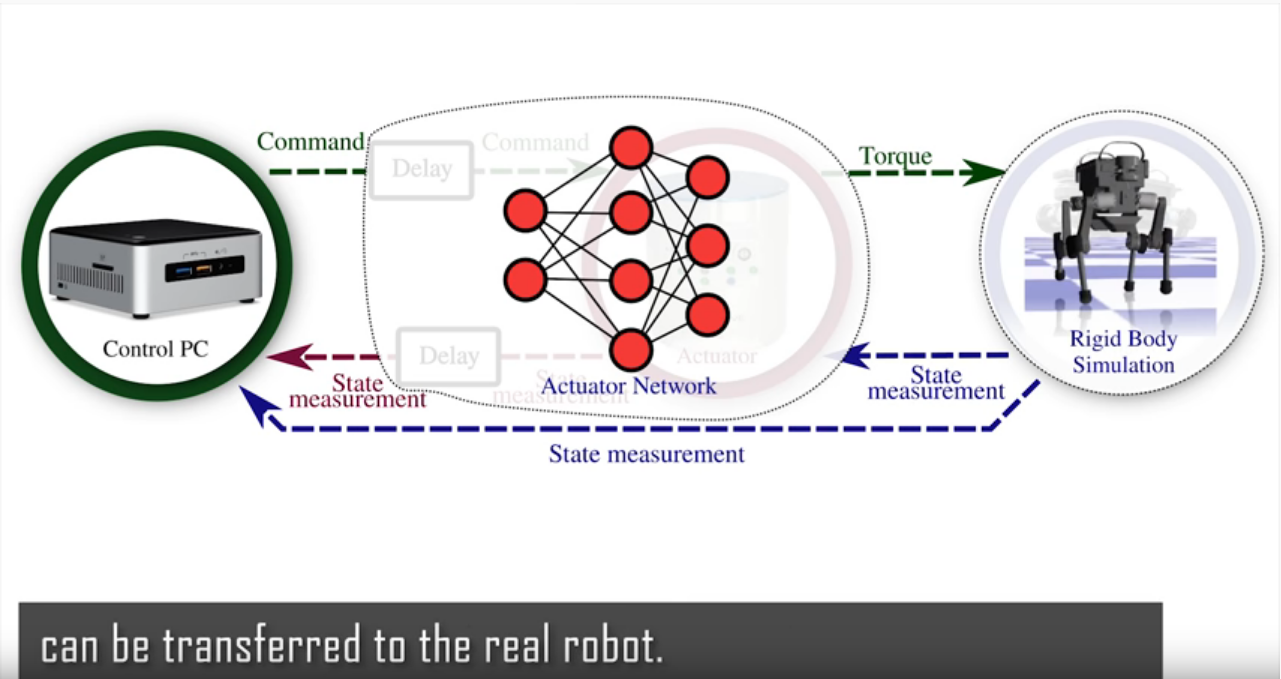
\includegraphics[width=0.70\textwidth]{Figures/robotWalking}
    \end{center}

\end{frame}

\section{iv. Frameworks for DRL}

\begin{frame}{Open Source frameworks}
    Several Open Source frameworks. Among others:
    
    \begin{itemize}
        \item Tensorforce, \url{https://github.com/tensorforce/tensorforce}.
        \item stable-baselines, \url{https://github.com/hill-a/stable-baselines}.
    \end{itemize}
    
    Workflow:
    
    \begin{itemize}
        \item Build your application-specific environment by filling in a class.
        \item Use built-in Agent (PPO, DQN, other) and built-in training functions to write a training script.
        \item Train.
        \item Evaluate in deterministic mode.
    \end{itemize}
    
    Moving from a framework to another is very little work (a few copy-pastes), because
    all what is needed is to implement [state, action, reward, terminal] communication.
\end{frame}


\begin{frame}{Frameworks: environment class in tensorforce}
    Full specification at: \url{https://github.com/tensorforce/tensorforce/blob/master/tensorforce/environments/environment.py} . \\~\\
    
    \tiny{
        \lstinputlisting[language=Python]{example_tensorforce.py}
    }
\end{frame}

\begin{frame}{Frameworks: environment class in gym}
    Full specification at: \url{https://github.com/openai/gym/blob/master/gym/core.py} . \\~\\

    \tiny{
        \lstinputlisting[language=Python]{example_gym.py}
    }
\end{frame}


\section{v. Why relevant for future}

\begin{frame}{ANNs, computing power, CPUs, GPUs, Moore's law}
    Increasingly attractive to use ANNs: the Moore's law is NOT dead yet. But one thread, free performance updates are dead.

    \begin{center}
      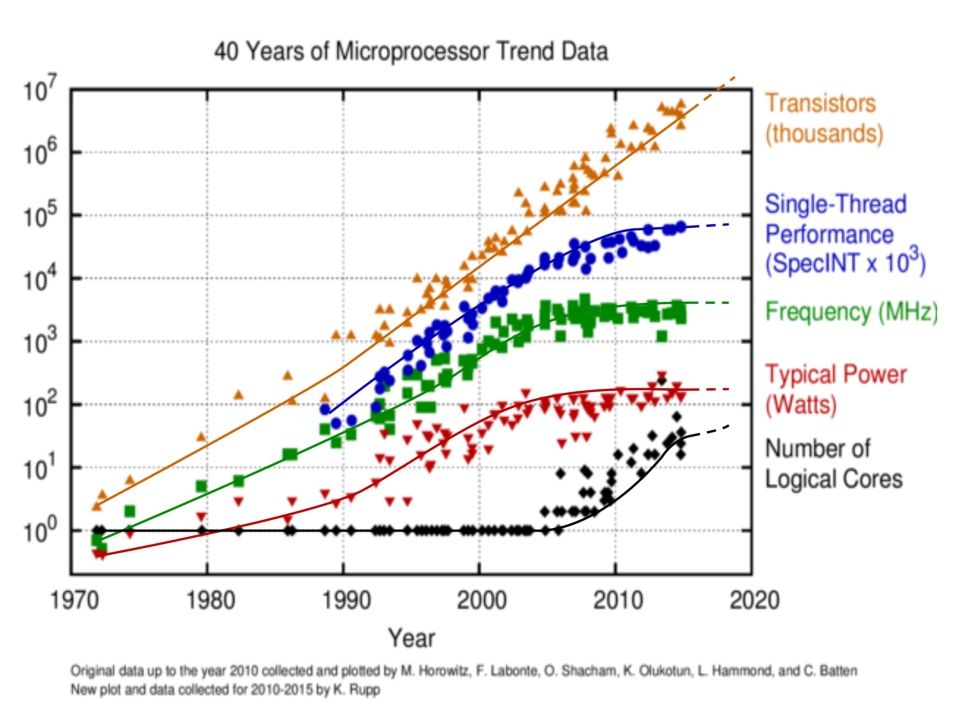
\includegraphics[width=0.65\textwidth]{./Figures/CPUs_vs_GPUs/40_years_trend}
    \end{center}

    Power limitations is the new wall computing power is hitting.
\end{frame}



\begin{frame}{Dennard scaling and the energy wall}
    Moore's law holds, Dennard scaling is dead.

    \begin{center}
        \textit{''Moore's law gives ut more transistores, Dennard scaling makes it useful''}, Bob Colwell, chief engineer P. II, P. III, P. 4, Intel; \\ Director of the Microsystems Technology Office, DARPA.
    \end{center}

    \begin{center}
      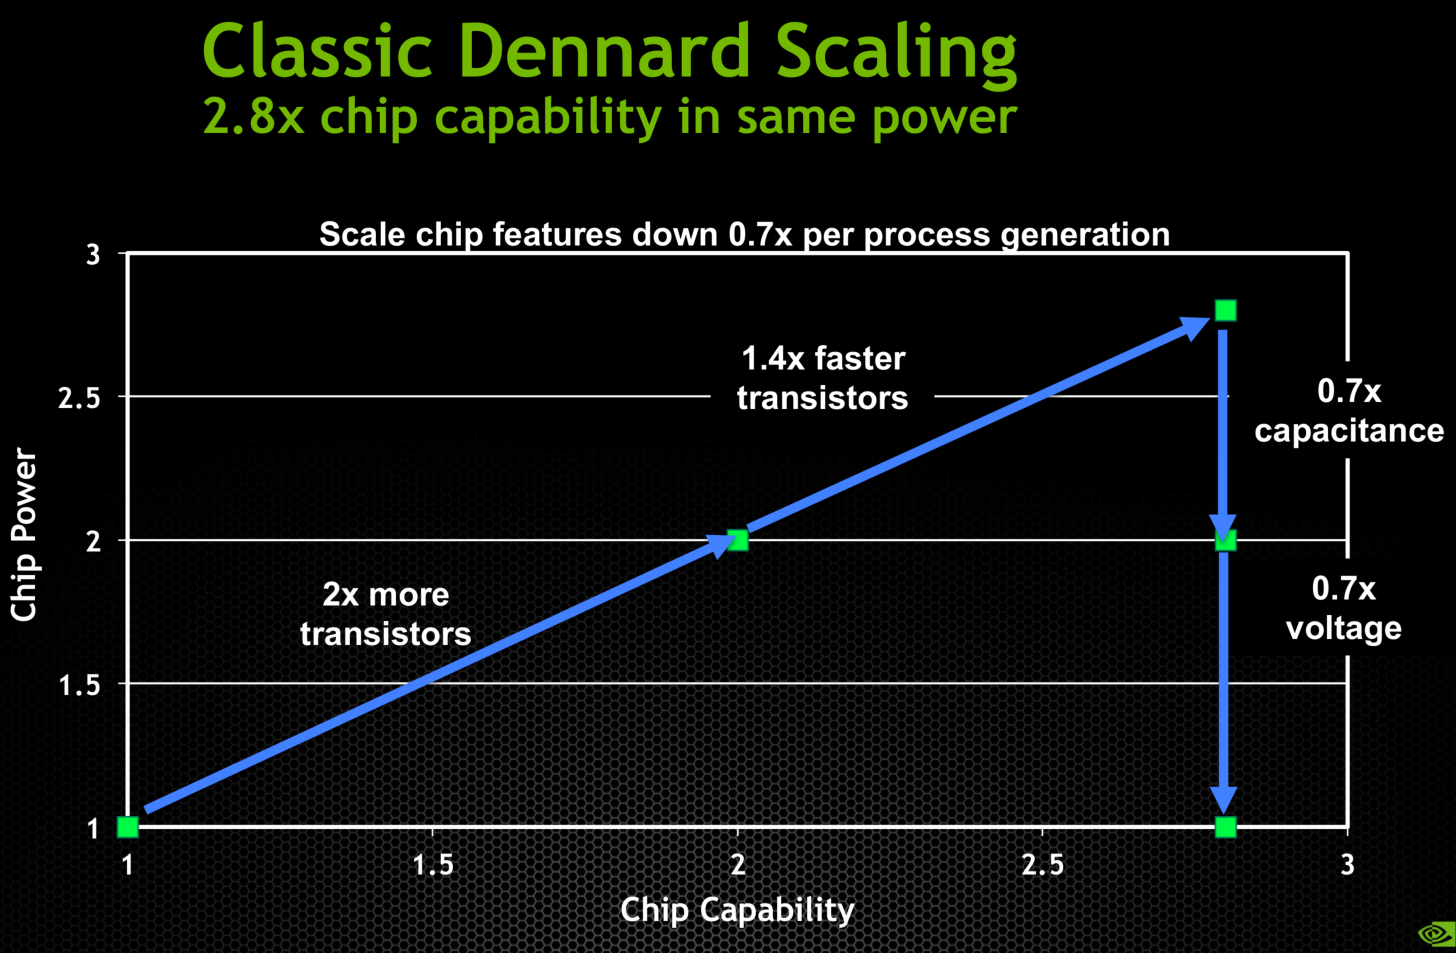
\includegraphics[width=0.69\textwidth]{./Figures/CPUs_vs_GPUs/classic_dennard}
    \end{center}
\end{frame}



\begin{frame}{Towards massively parallel future}
    Many problems: power dissipation wall, dark silicon, etc. \\

    CPU: $1700$ pJ/Op, GPU: $160$ pJ/Op, ASIC: $<10$ pJ/Op.

    \begin{center}
      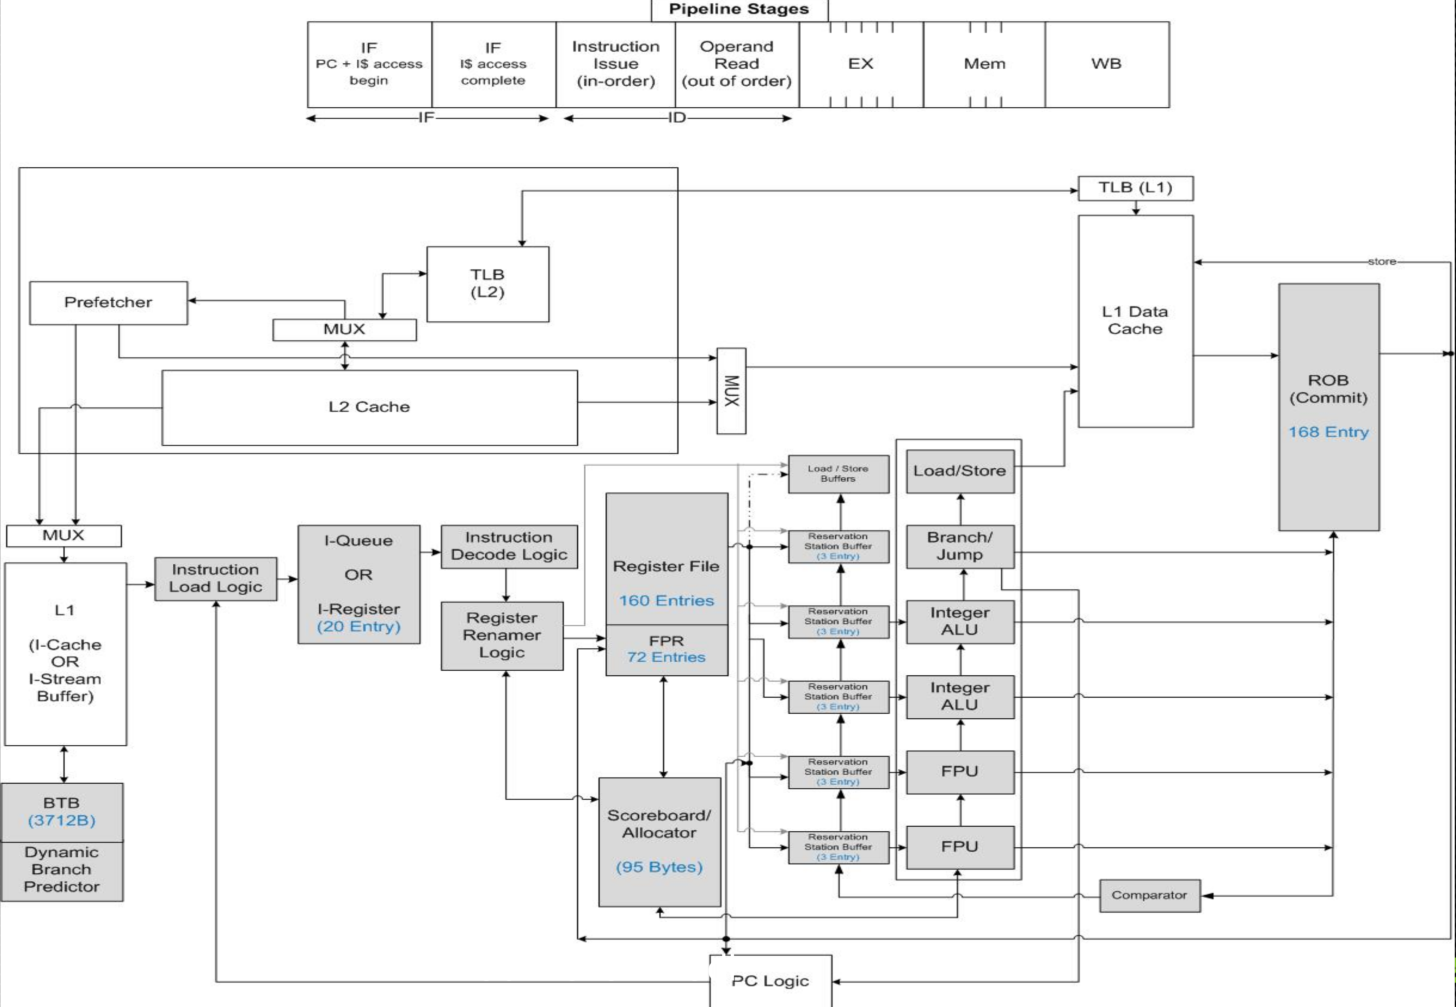
\includegraphics[width=0.58\textwidth]{./Figures/CPUs_vs_GPUs/overview_architecture}
    \end{center}

    Do like the brain: low frequency, high latency, highly parallel, very large computation power, very energy efficient.

    \begin{center}
      Need adapted algos to take advantage of computing power increases.
    \end{center}
\end{frame}


\begin{frame}{AI and compute}
"AI and compute", Dario Amodei et. al., OpenAI blog, 2018.

\begin{center}
  "[...] since 2012, the amount of compute in the largest AI training runs has been increasing exponentially with a 3.4-month doubling time (by comparison, Moore's Law had a 2-year doubling period)".
\end{center}

\begin{center}
        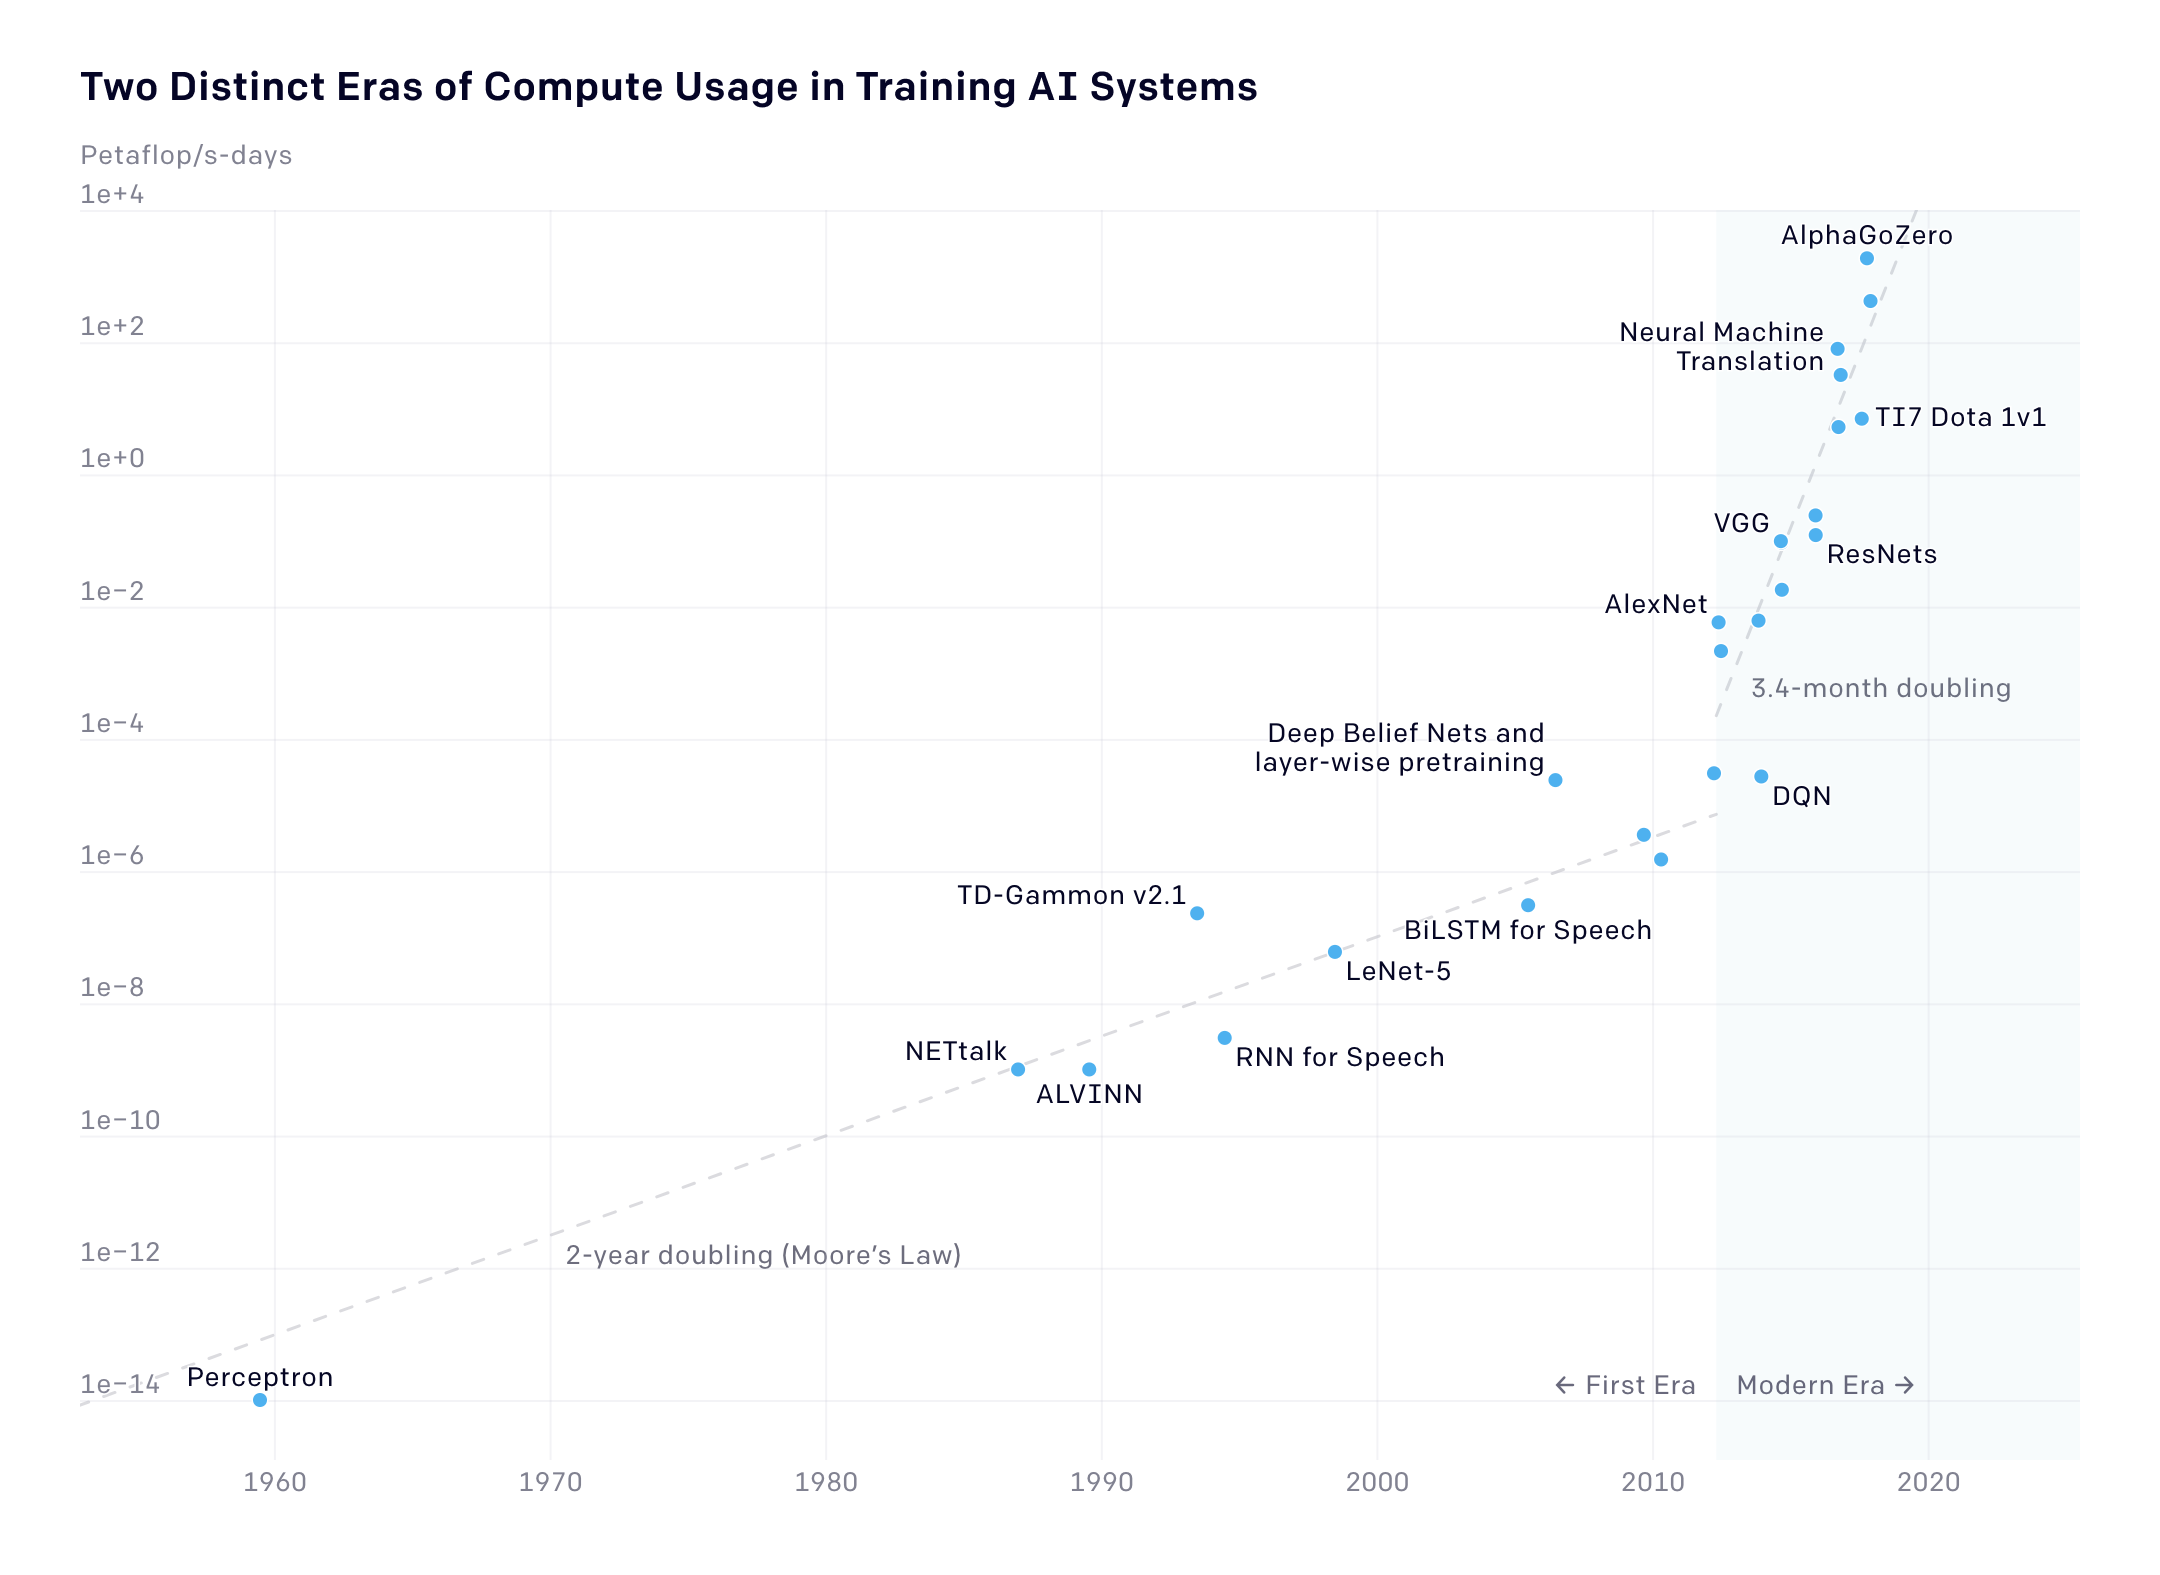
\includegraphics[width=0.49\linewidth]{Figures/ai-and-compute-all}
		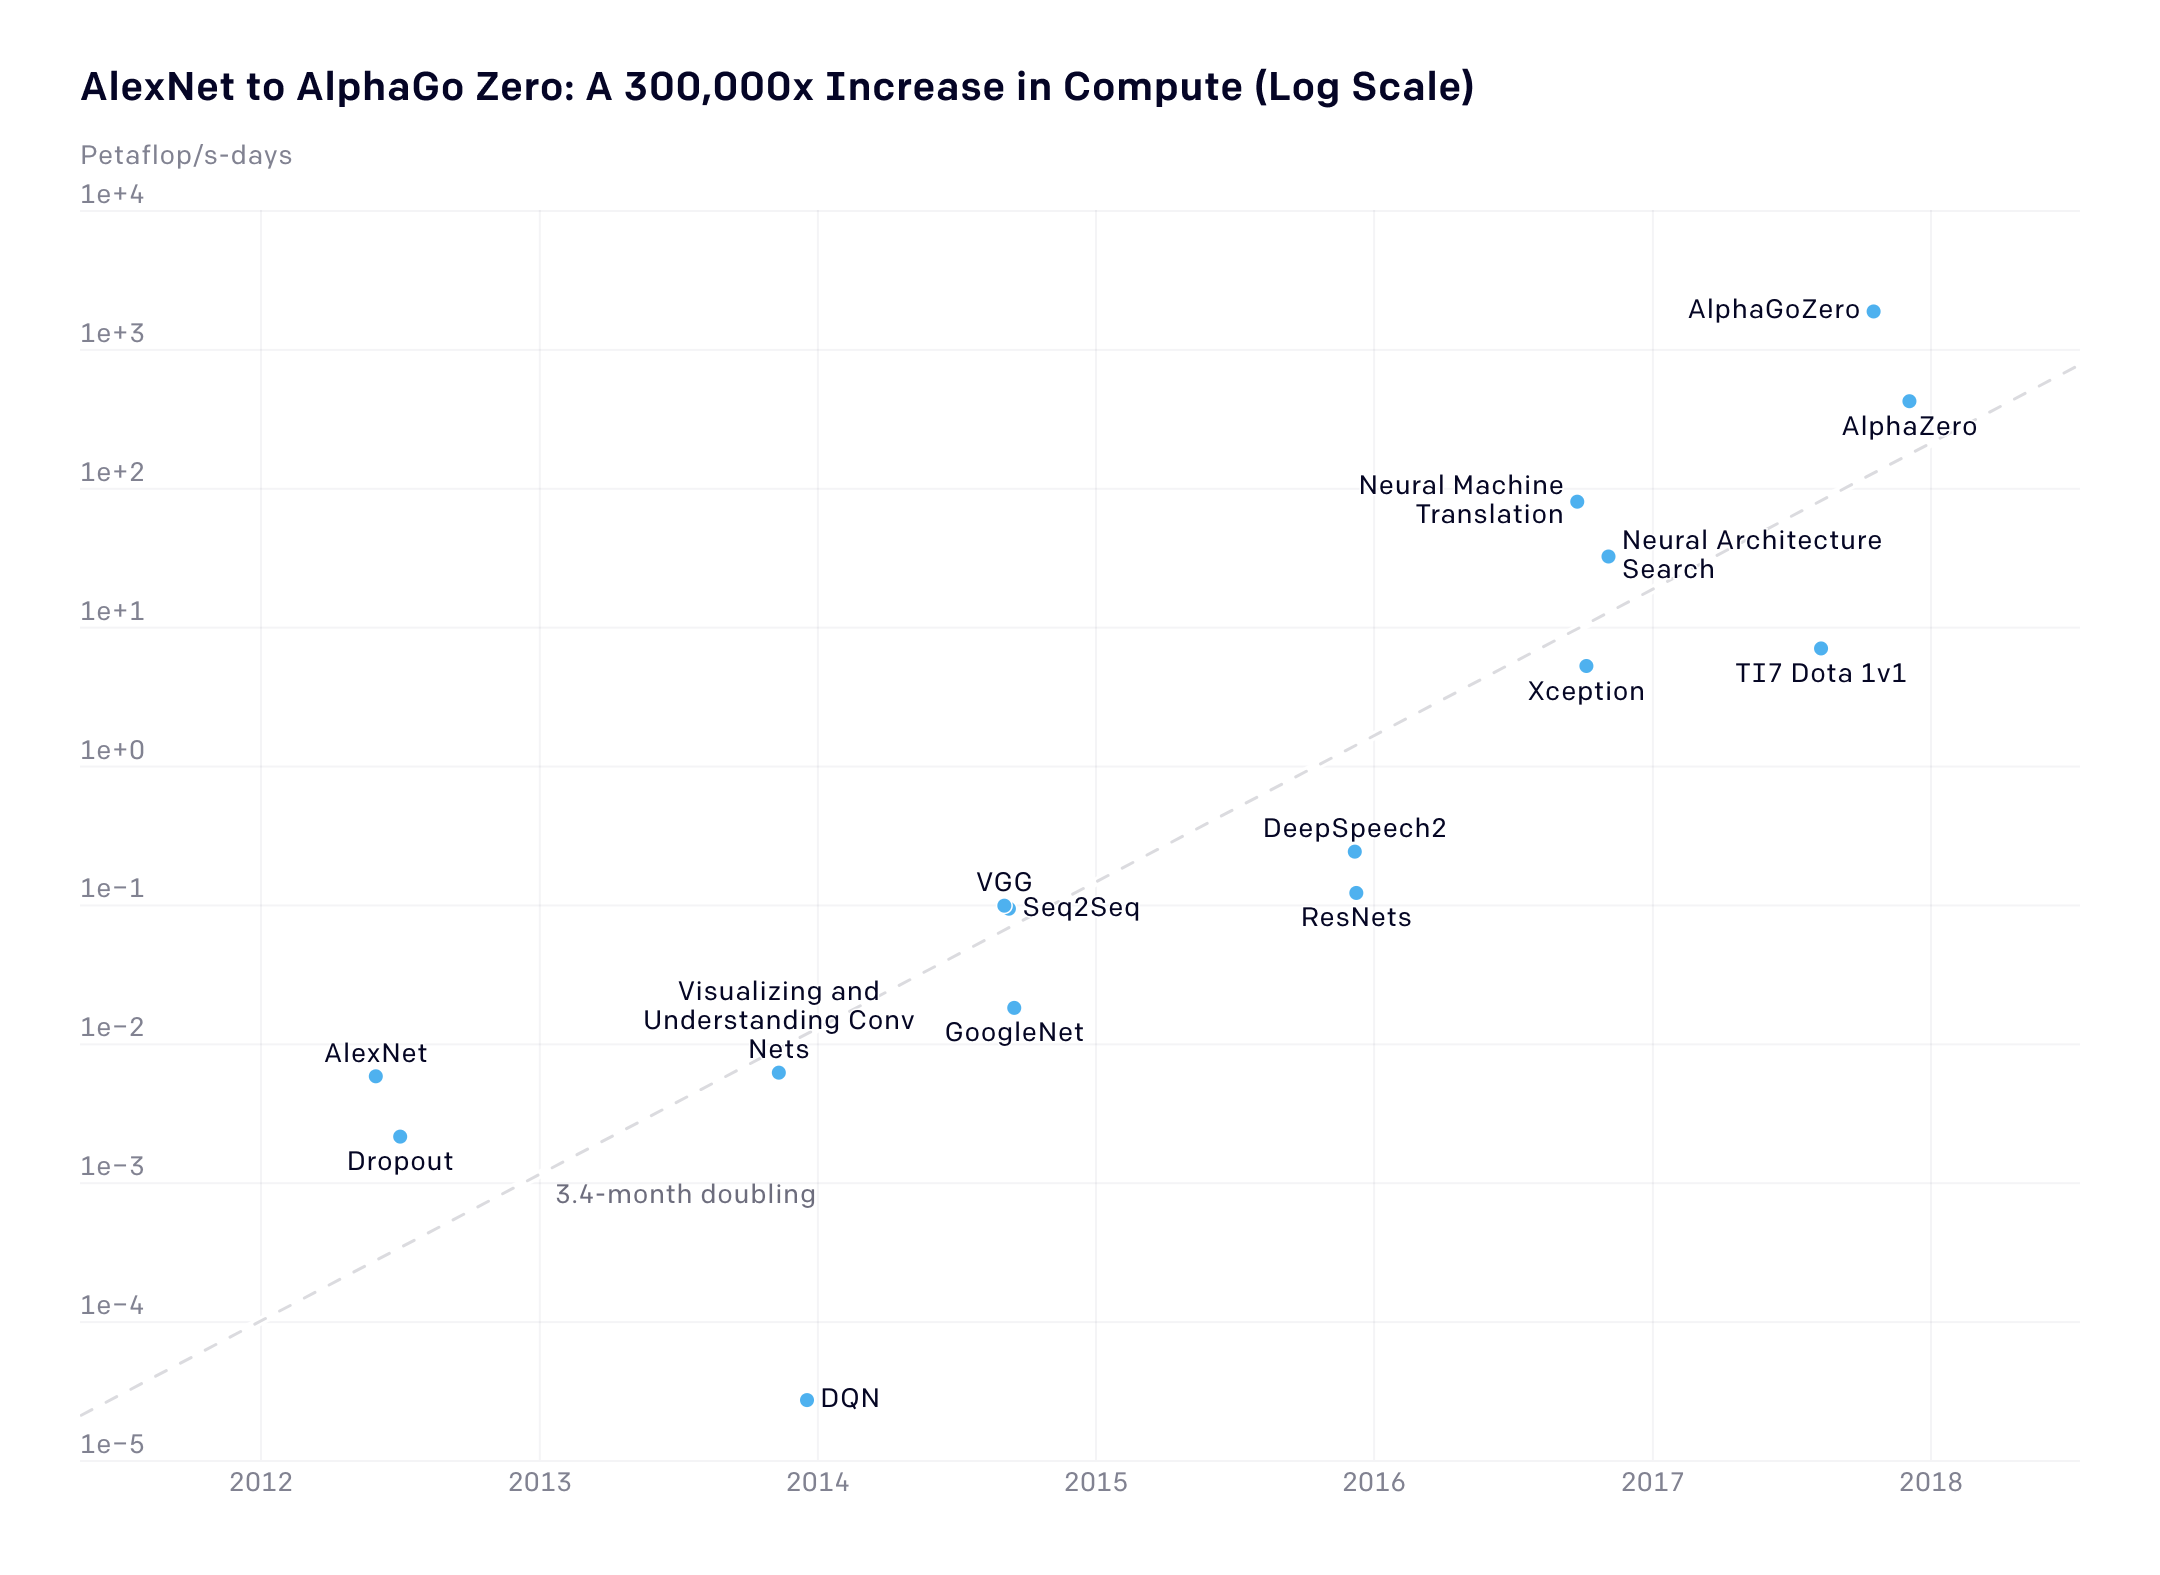
\includegraphics[width=0.49\linewidth]{Figures/ai-and-compute-modern-log}
\end{center}

CPU to GPU to large-scale GPU clusters to large-scale ASIC clusters.

\end{frame}

\begin{frame}{ANNs and computational power}
Difficult to take full advantage of large parallel systems:
\begin{itemize}
    \item Some problems cannot be parallelized.
    \item Parallelizable problems may be hard to make scale.
    \item HPC is quite hard.
\end{itemize}

But ANNs / DRL are naturally well adapted to such architectures.

\begin{itemize}
    \item Based on small computational units.
    \item Batch updates is naturally parallel.
    \item An ASIC ANN design can be used to solve many problems thanks to the generality of ANNs.
\end{itemize}
\end{frame}

\begin{frame}{Increasing efficiency of learning algorithms}
\begin{center}
		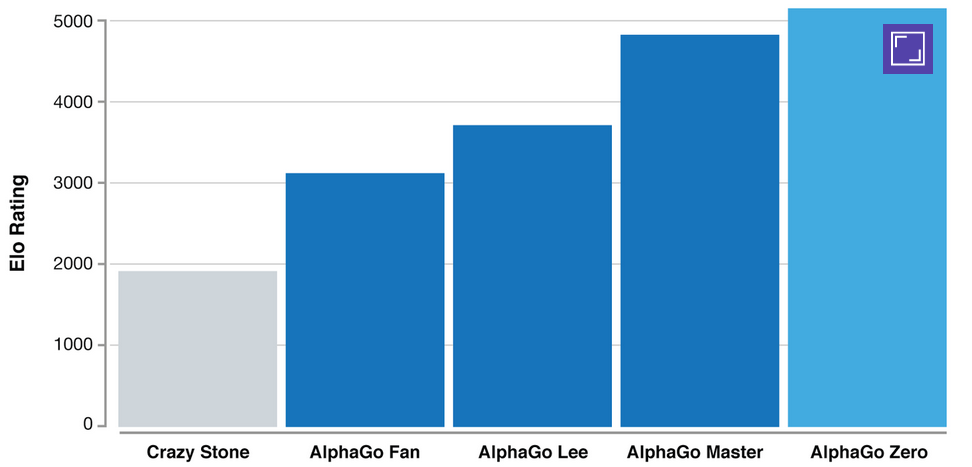
\includegraphics[width=0.58\linewidth]{Figures/ELO_ranking_DRL} \\
		\includegraphics[width=0.58\linewidth]{Figures/power_consumption_DRL}
	\end{center}
	{\tiny Figures from Google Brain blog.}
\end{frame}

\section{Deep Reinforcement Learning for Active Flow Control}

\begin{frame}{DRL for turbulence control and active flow control?}
    \begin{itemize}
        \item DRL is the natural candidate for AFC and turbulence control: need to both find and express a solution.
    \end{itemize}

    \begin{center}
    Several recent works suggest it is a promising approach:
    \end{center}

    'Artificial Neural Networks trained through Deep Reinforcement Learning discover control strategies for active flow control', Rabault et. al., JFM (2019). \\~\\

    'Accelerating Deep Reinforcement Leaning strategies of Flow Control through a multi-environment approach', Rabault and Kuhnle, PoF (2019). \\~\\

    'Control of chaotic systems by Deep Reinforcement Learning', Bucci et. al., PoRS-A (2019). \\~\\

    'Reinforcement learning versus linear control of Rayleigh Benard convection', G. Beintema et. al., ETC2019.
\end{frame}


\begin{frame}{Karman vortex street and the Turek benchmark}
    \begin{center}
        Karman vortex street is emblematic of Fluid Mechanics.
    \end{center}

     \begin{center}
      \includegraphics[width=0.35\textwidth, height=2cm]{./Figures/karman_in_Nature}
      \hspace{0.05cm}
      \includegraphics[width=0.35\textwidth, height=2cm]{./Figures/Karman_in_experiment}
    \end{center}

    Thereafter: 2D FEniCS at $Re = \bar{U} L / \nu = 100$: laminar unsteady, as in:

    \begin{center}
        'Benchmark Computations of Laminar Flow Around a Cylinder', \textit{Sch\"afer and Turek}, Flow Sims. with High-Perf. Computers (1996).
    \end{center}

    \begin{center}
      \includegraphics[width=0.85\textwidth, height=2cm]{./Figures/probe_position_pressure}
    \end{center}

    Add velocity probes ($s_t$), normal jets ($a_t$), reduce $C_D = \frac{D}{1/2 \rho U^2 D_C}$ ($r_t$).
\end{frame}


\begin{frame}{Re 100}
    'Artificial Neural Networks trained through Deep Reinforcement Learning discover control strategies for active flow control', Rabault et. al., JFM (2019). \\

    \begin{center}
  \movie[
    height = 4.8cm,
    width = 10.5cm,
    showcontrols,
    autostart=True,
    repeat,
    poster
  ]
  {https://youtu.be/0QbKk5SzMws}{./comparison_baseline_actuation.avi}
\end{center}
    Full code on github: \url{https://github.com/jerabaul29/Cylinder2DFlowControlDRL}
\end{frame}


\begin{frame}{What is happening?}
    Very small jets allow for 'boat tailing'. Already solving a difficult task!

    \begin{figure*}
    \begin{center}
      \includegraphics[width=.70\textwidth]{Figures/pressure_difference}
    \end{center}
    \end{figure*}

    \begin{figure*}
    \begin{center}
      \includegraphics[width=.51\textwidth]{Figures/drag_and_jets}
    \end{center}
    \end{figure*}
\end{frame}

\begin{frame}{How good is the strategy? (I)}
    Get about 8\% drag reduction. How good is that? \\~\\
    
    Drag is due to the 'base flow' and 'vortex shedding' components:
    
    $$C_D = C_D^{base flow} + C_D^{shedding}$$
    
    Control can only affect $C_D^{shedding}$ ("Optimal rotary control of the cylinder wake using proper orthogonal decomposition reduced-order model", Bergmann et. al., PoF, 2005):
    
    \begin{figure*}
    \begin{center}
      \includegraphics[width=.51\textwidth]{Figures/illustration_Cordier}
    \end{center}
    \end{figure*}
\end{frame}

\begin{frame}{How good is the strategy? (II)}
     Estimate $C_D^{base flow}$ in our case from an axisymmetric simulation (symmetric BC on lower border):
     
     \begin{figure*}
    \begin{center}
      \includegraphics[width=.99\textwidth]{Figures/base_flow_half_domain}
    \end{center}
    \end{figure*}
    
    $2 C_D^{half-domain} = 2.93$,~ $<C_D^{no control}> = 3.205$,~ $<C_D^{control}> = 2.95$. \\~\\
    
    Suppressed 93 \% of the vortex-shedding-induced drag.
\end{frame}

\begin{frame}{We still need engineers (I)}
    Choice of the reward function: prevent 'cheating'.

\begin{equation} r = \langle D \rangle_{S} - \alpha |\langle L\rangle_{S}|, \label{reward_function} \end{equation}

    \begin{figure*}
    \begin{center}
      \includegraphics[width=.75\textwidth]{Figures/fig5_illustration_cheating}
    \end{center}
    \end{figure*}
\end{frame}

\begin{frame}{We still need engineers (II)}
    \begin{figure*}
    \begin{center}
      \includegraphics[width=.45\textwidth]{Figures/fig2_illustration_2_time_scales}
    \end{center}
    \end{figure*}

    Choose the right characteristic timescale!

    \begin{figure*}
    \begin{center}
      \includegraphics[width=.40\textwidth]{Figures/fig6_fig_effect_action_frq}
    \end{center}
    \end{figure*}

    Of course, can predict action duration...
\end{frame}



\begin{frame}{Flexible method}
Flexible to look at different cases: small control cylinders \\ (credit: Wei Zhang). \\~\\

    \begin{figure*}
    \begin{center}
      \includegraphics[width=.99\textwidth]{Figures/FlowUncontrolled} \\
      \includegraphics[width=.99\textwidth]{Figures/FlowControlled}
    \end{center}
    \end{figure*}
\end{frame}


\begin{frame}{Challenge I. Towards higher Re: faster learning}
    Parallelize collection of trajectories in the phase space during training. \\~

    'Accelerating Deep Reinforcement Leaning strategies of Flow Control through a multi-environment approach', Rabault and Kuhnle, PoF (2019). \\

    \begin{figure*}
    \begin{center}
      \includegraphics[width=.49\textwidth]{Figures/fig_real_time_under}
      \includegraphics[width=.49\textwidth]{Figures/fig_real_time_over}
    \end{center}
    \end{figure*}

    Speedup x60. Code fully available on github: \\
    {\small \url{https://github.com/jerabaul29/Cylinder2DFlowControlDRLParallel}}
    
\end{frame}


\begin{frame}{Controlling more challenging flows: Re 500}
    Ongoing work, collaboration with Nanjing Univ. of Aero. and Astro. \\

    Much stronger separation, so stronger jets and more unstable - but some promising preliminary results.

    \begin{center}
  \movie[
    height =6cm,
    width = 9.5cm,
    showcontrols,
    autostart=True,
    repeat,
    poster
  ]
  {https://youtu.be/PDyr6CHIwVk}{./Re_500.avi}
\end{center}
\end{frame}


\begin{frame}{Complex dynamics at Re 500}
    Already at Re 500, the dynamics start to be more complex:

    \begin{figure*}
    \begin{center}
      \includegraphics[width=.32\textwidth]{Figures/both_drag}
      \includegraphics[width=.32\textwidth]{Figures/both_lift}
      \includegraphics[width=.32\textwidth]{Figures/both_area}
    \end{center}
    \end{figure*}

    \begin{itemize}
        \item Very large changes in recirculation area.
        \item Non pseudo-periodic behavior, large frequency shift.
        \item Violent instability and collapse of the wake.
    \end{itemize}

    Currently working on keeping stable control also for later times. Going to higher Re / 3D flows will require another solver.

\end{frame}



\begin{frame}{Learning `global' control policies}
  'Robust active flow control over a range of Reynolds numbers using an artificial neural network trained through deep reinforcement learning', Tang et. al., PoF (2020). \\
  
  \begin{figure*}
    \begin{center}
      \includegraphics[width=.49\textwidth]{Figures/baseline_Case_109_four_Res}
      \includegraphics[width=.49\textwidth]{Figures/CD_comparison_general_model_Case_109_vorticity}
    \end{center}
    \end{figure*}
    
    1 ANN, control at all Res within training range efficiently.
\end{frame}


\begin{frame}{Using another solver for higher Res: LBM}
  Collaboration Hong Kong Polytechnic Univ. \\
  R. Feng, J. Rabault, H. Tang (under writing). \\
  
  \\~\\
  
  Combine parallelism at simulation level and faster CFD:
  \begin{itemize}
    \item Reproduce (much quicker) Re 100 results.
    \item Extend to higher Re: 1000 (but in 2D).
    \item Strongly pseudo-chaotic.
  \end{itemize}
\end{frame}

{
\setbeamercolor{background canvas}{bg=}
\includepdf[pages=1]{Figures/HiFiCoMa-1.pdf}
}

{
\setbeamercolor{background canvas}{bg=}
\includepdf[pages=1]{Figures/HiFiCoMa-12.pdf}
}

{
\setbeamercolor{background canvas}{bg=}
\includepdf[pages=1]{Figures/HiFiCoMa-14.pdf}
}



\begin{frame}{Challenge II. How to increase the number of controls? Example of falling fluid film.}
  "Exploiting locality and physical invariants to design effective Deep Reinforcement Learning control of the unstable falling liquid film", Belus et. al., ArXiv (2019), accepted AIP-A.
  
  Use simulation from "An ensemble method for sensor optimisation applied to falling liquid films", Z. Che et. al., IJMFF (2014):
  
  \begin{equation*}
    \frac{\partial h}{\partial t} + \frac{\partial q}{\partial x} = 0, \newline
    \frac{\partial q}{\partial t} + \frac{6}{5} \frac{\partial}{\partial x} \left( \frac{q^ 2}{h} \right) = \frac{1}{5 \delta} \left( h \frac{\partial^3 h}{\partial x^3} + h - \frac{q}{h^2} \right),
\end{equation*}

with $\delta = (\rho H_c^{11}g^4/ \sigma)^{1/3} /45 \nu^2$.

    \begin{figure*}
    \begin{center}
      \includegraphics[width=.92\textwidth]{Figures/regions_}
    \end{center}
    \end{figure*}
\end{frame}

\begin{frame}{How to insert several jets? (M1)}
Naive approach: large inputs and outputs. \\

  \begin{figure*}
    \begin{center}
      \includegraphics[width=.98\textwidth]{Figures/graph_mlp_final}
    \end{center}
    \end{figure*}
    
Curse of dimensionality on the number of jets:

    \begin{itemize}
        \item For thought experiment, p possible jet strengths.
        \item Use N jets, and a fully connected ANN.
        \item Then, need to fully explore:
    \end{itemize}

    \begin{center}
        $C = p^N $ combinations!
    \end{center}

    Of course, we can do much better...
\end{frame}

\begin{frame}{How to insert several jets? (M2)}
Smarter approach: use a fully convolutional network. \\

Respect invariance by translation. \\

  \begin{figure*}
    \begin{center}
      \includegraphics[width=.98\textwidth]{Figures/graph_cnn_final}
    \end{center}
    \end{figure*}
   
This way, truly learn only 1 set of weights. Take advantage of translational invariance.
\end{frame}

\begin{frame}{How to insert several jets? (M3)}
Even better: split the simulation into cloned environments. \\

This way, provide both invariance and more reward signal. \\

  \begin{figure*}
    \begin{center}
      \includegraphics[width=.98\textwidth]{Figures/graph_multienv_final}
    \end{center}
    \end{figure*}
\end{frame}

\begin{frame}{Comparing M1, M2, M3}
\begin{figure*}
    \begin{center}
      \includegraphics[width=.43\textwidth]{Figures/figure_nice1jet_}
      \includegraphics[width=.43\textwidth]{Figures/figure_nice5jet_} \\
      \includegraphics[width=.43\textwidth]{Figures/figure_nice10jet_}
      \includegraphics[width=.43\textwidth]{Figures/figure_nice20jet_}
    \end{center}
    \end{figure*}
\end{frame}

\begin{frame}{M3 can handle arbitrary number of jets}

With M3, for N jets, perform N actions per simulation advance. \\~\\

Cost of learning $\propto$ [number of simulation advances] rather than to [number of actions]. 

\begin{figure*}
    \begin{center}
      \includegraphics[width=.48\textwidth]{Figures/figure_comparison_njet_m31}
      \includegraphics[width=.48\textwidth]{Figures/figure_comparison_njet_m30}
    \end{center}
    \end{figure*}
    
Constant cost of learning for any number of jets. Makes sense physically.    
\end{frame}

\begin{frame}{Satisfactory control}
    Control from the start location of instability development:
    
\begin{center}
  \includegraphics[width=.75\textwidth]{Figures/trained}
\end{center}
    
    Control in an area where large interfacial waves are present:
    
\begin{center}
  \includegraphics[width=.85\textwidth]{Figures/figure5-1}
\end{center}
\end{frame}

\begin{frame}{Confronting some of the difficulties of turbulence: multi-modality with weak coupling}
    Difficulties with turbulence: multi-modality with weak coupling. \\

    Nonlinear crosstalks system of 'Machine Learning Control-Taming Nonlinear Dynamics and Turbulence', Duriez, Brunton and Noack (2016):

\begin{align}
    \frac{da_1}{dt} &= \sigma a_1 - a_2 \\
    \frac{da_2}{dt} &= \sigma a_2 + a_1 \\
    \frac{da_3}{dt} &= -0.1 a_3 - 10 a_4 \\
    \frac{da_4}{dt} &= -0.1 a_4 + 10 a_3 + b \\
    \sigma &= 0.1 - a_1^2 - a_2^2 - a_3^2 -a_4^2,
    \label{eqn:cross_talks}
\end{align}

Coupling disappears if linearize in a state where initially $a_3 = a_4 = 0$.

Measure quality of control: $J = \overline{a_1^2 + a_2^2} + \gamma \overline{b^2}$.
    
\end{frame}


\begin{frame}{Results}
    Manage to control with DRL:

    \begin{figure*}
    \begin{center}
      \includegraphics[width=.42\textwidth]{Figures/reward_convergence_with_inset} \\
      \includegraphics[width=.42\textwidth]{Figures/control}
      \includegraphics[width=.42\textwidth]{Figures/controlled}
    \end{center}
    \end{figure*}

\end{frame}

\section{DRL for shape optimization}

\begin{frame}{Can we learn to produce lift in a simulation?}
    We take wings for granted, but took a long time to 'discover' / 'invent'. \\
    Do we really know that a wing is the best solution?

    \begin{center}
        Use DRL to produce lift.
    \end{center}

    J. Viquerat, J. Rabault, et. al. "Direct shape optimization through Deep Reinforcement Learning"

    \begin{figure*}
    \begin{center}
      \includegraphics[width=.72\textwidth]{Figures/simulation_setup}
    \end{center}
    \end{figure*}
\end{frame}

\begin{frame}{Shape parametrization}
    \begin{itemize}
        \item Bezier curves.
        \item Start from a cylinder.
        \item Each point allowed to be moved in a torus domain.
        \item Punish 'bad', i.e. non meshing, shapes.
    \end{itemize}

    \begin{center}
      \includegraphics[width=.78\textwidth]{Figures/shape_discretization}
    \end{center}
\end{frame}

\begin{frame}{Reward and normalization}
    \begin{itemize}
        \item Need a 'normalized' reward to avoid simple blowing up of the shape.
        \item Normalize inputs / outputs to keep ANN inputs / outputs in [-1, 1].
    \end{itemize}


\begin{equation}
\label{eq:reward_wing}
	r_t = \left< \frac{C_l}{\left| C_d \right|} \right> - \left< \frac{C_l}{\left| C_d \right|} \right>_{\text{cyl}},
\end{equation} 

\begin{equation}
	\left\{
	\begin{aligned}
		r &= r_{\text{max}} \max \left( \left| p \right|, r_{\text{min}} \right),\\
		\theta &= \frac{\pi}{n} \left( i + \frac{q}{2} \right),\\
		x &= r \cos \left( \theta \right),\\
		y &= r \sin \left( \theta \right),\\
		e &= \frac{1}{2} \left(1 + r \right).
	\end{aligned}
	\right.
\end{equation}

\end{frame}

\begin{frame}{Results}
    \begin{center}
      \includegraphics[width=.65\textwidth]{Figures/results_shape_opt}
    \end{center}
\end{frame}

\begin{frame}{Future improvements}
    \begin{itemize}
        \item Use a level-set line to deform mesh.
        \item ANN sees many configurations and optimize.
    \end{itemize}

    We want to use the ANN to produce an 'intuition'. Think about the drag reduction on a truck:

    \begin{itemize}
        \item Strongly nonlinear: changing the front affects the flow at the back.
        \item Gradient descent \ adjoint method do not work: too many local extrema.
        \item For now: human experts with years of experience.
    \end{itemize}

    DRL would scale better than human experts.
\end{frame}

\section{Other applications in the literature}

\section{i. Rayleigh-Benard instability control}

\begin{frame}{Rayleigh-Benard instability and manufacturing of monochristals}

    "Reinforcement learning versus linear control of Rayleigh-Benard convection", G. Beintema et. al., ETC2019.
    
    \begin{figure*}
    \begin{center}
      \includegraphics[width=.45\textwidth]{Figures/RBi}
      \hspace{1cm}
      \includegraphics[width=.35\textwidth]{Figures/monochristal}
    \end{center}
    \end{figure*}
    
    
    \begin{center}
https://www.youtube.com/watch?v=Ju7JyFgvqFc \\~\\
https://www.youtube.com/watch?v=UjGd1if99jg
     
    \end{center}

    Successful control while traditional methods do not work.
\end{frame}


\section{ii. Optimal navigation: the Zemelo problem}

\begin{frame}{Optimal traveling}

"Zermelo problem: Optimal point-to-point navigation in 2D turbulent flows using
Reinforcement Learning", Biferale et. al., Chaos: Interdisciplinary Journal of Nonlinear Science 29:10 (2019).

    \begin{figure*}
    \begin{center}
      \includegraphics[width=.91\textwidth]{Figures/Zemelo_1}
    \end{center}
    \end{figure*}
\end{frame}

\begin{frame}{Optimal traveling}
    \begin{figure*}
    \begin{center}
      \includegraphics[width=.45\textwidth]{Figures/Zemelo_2} \\
      \includegraphics[width=.65\textwidth]{Figures/Zemelo_3}
    \end{center}
    \end{figure*}
\end{frame}

\section{iii. Optimal swimming of fishes}

\begin{frame}{Group swimming}
    \begin{figure*}
    \begin{center}
      \includegraphics[width=.95\textwidth]{Figures/fish_article2} \\
    \end{center}
    \end{figure*}

"Efficient collective swimming by harnessing vortices through deep reinforcement learning", Verma et al., PNAS (2018)
\end{frame}

\section{iv. Control of chaotic systems}



\begin{frame}{Control of chaotic systems}
"Control of chaotic systems by deep reinforcement learning", Bucci et. al., PoRSA (2019).

Control the 1D Kuramoto-Sivashinsky model using DDPG.

\begin{figure*}
    \begin{center}
      \includegraphics[width=.75\textwidth]{Figures/ControlChaoticSystemsIllustration}
    \end{center}
    \end{figure*}

\end{frame}




\section{v. Control of AUVs}


\begin{frame}{Attitude control of drones}
"Deep Reinforcement Learning Attitude Control of Fixed-Wing UAVs Using Proximal Policy Optimization", Bohn et. al., 2019 International Conference on Unmanned Aircraft Systems (ICUAS). IEEE (2019). 

\begin{figure*}
    \begin{center}
      \includegraphics[width=.75\textwidth]{Figures/PID_vs_PPO_attitude_control}
    \end{center}
    \end{figure*}
\end{frame}



\section{vi. Control of glider}


\begin{frame}{Glider soaring}
"Glider soaring via reinforcement learning in the field", Reddy et. al., Nature (2018).

\begin{figure*}
    \begin{center}
      \includegraphics[width=.55\textwidth]{Figures/soaring_glider}
    \end{center}
    \end{figure*}
\end{frame}


\section{vii. Optimal design of missiles}

\begin{frame}{Missiles and RL}
"Aerodynamic shape optimization using a novel optimizer based on machine learning techniques", X. Yan et. al. \\
    
    \begin{figure*}
    \begin{center}
      \includegraphics[width=.95\textwidth]{Figures/MissileOptimization} \\
    \end{center}
    \end{figure*}
\end{frame}

\section{viii. Growing interest}

\begin{frame}{APS - DFD}

{\small
2018: 1 abstract about DRL (mine). \\~\\

2019: 10 abstracts (details: \url{http://meetings.aps.org/Meeting/DFD19}):

\begin{itemize}
\item Airfoil Shape Optimization using Deep Q - Network

\item Airfoil control with Proximal Policy Optimization

\item Zermelo's problem: Optimal point-to-point navigation in 2D turbulent flows using Reinforcement Learning

\item Suppressing flow separation over a flat plate using machine learning

\item Reinforcement Learning for a Bio-Inspired Vehicle with Undulating Fin Propulsion.

\item Reinforcement learning enabled control of chaotic dynamics

\item Elimination of velocity deficit behind a cylinder using reinforcement learning

\item Deep Reinforcement Learning for Flow Control

\item Reinforcement learning enabled control of chaotic dynamics

\item Predator-Prey Interactions using Deep Reinforcement Learning
\end{itemize}
}
\end{frame}

\section{Conclusion}

\begin{frame}{Summary of the results and general considerations}
    \begin{itemize}
      \item Effective for control of non-linear, high dimensional systems.
      \item Many advantages, compared with for example adjoint method: train once use many times, closed loop, partial observation, transfer learning, extrapolation, 'trivially' parallel training algorithm.
    \end{itemize}

    More generally DRL is a nonlinear, non convex, general purpose optimizer: CFD engineer workflow can be seen as DRL.

    \begin{figure*}
    \begin{center}
      \includegraphics[width=.70\textwidth]{Figures/fixed_last}
    \end{center}
    \end{figure*}

    \begin{center}
        Finally a tool that could fully use actuations and design possibilities?
    \end{center}

\end{frame}



\begin{frame}{Strengths and weaknesses of DRL}
Weaknesses:

\begin{itemize}
    \item Needs lots of data.
    \item No guarantee of convergence / stability.
    \item Not (easily) explainable.
\end{itemize}

Strengths:

\begin{itemize}
    \item Seems to work quite well in practise.
    \item No need for full access to the system.
    \item Can (try to) extrapolate.
    \item Seems robust.
\end{itemize}

Sometimes unfair criticisms from reviewers / others:

\begin{itemize}
    \item "this is only gradient descent": true but false.
    \item "not explainable = no value": false, just one (experimental) tool.
\end{itemize}

\end{frame}




\begin{frame}{Future and perspectives}

Control may be for the time being the most promising avenue.

Recent results:

\begin{itemize}
    \item Proof-of-concept.
    \item Parallelization / speedup.
    \item Application to large systems / invariants.
\end{itemize}

Minor remaining questions; well adapted for MSc thesis, extend released code:

\begin{itemize}
    \item Robustness? (some preliminary work, mostly remains to be done).
    \item Interpolation / extrapolation of policies? (already done, to be released).
    \item Reality gap / experiment?
\end{itemize}

Major remaining works; need solvers, (many) CPUs, man-years:

\begin{itemize}
    \item 3D systems.
    \item Higher Re, possibly through experiences.
    \item Example I: sphere in 3D at moderate Re (already well advanced).
    \item Example II: BL and BL friction.
\end{itemize}

\end{frame}


\begin{frame}{Additional resources}

\begin{\itemize}
    \item Book chapter about DRL in fluid mechanics: \url{https://www.researchgate.net/publication/343934046_DEEP_REINFORCEMENT_LEARNING_APPLIED_TO_ACTIVE_FLOW_CONTROL}

    \item DRL control at Re 100: \url{https://github.com/jerabaul29/Cylinder2DFlowControlDRL}

    \item DRL control in parallel: \url{https://github.com/jerabaul29/Cylinder2DFlowControlDRLParallel}

    \item Robust DRL control over range of Res: \url{https://github.com/thw1021/Cylinder2DFlowControlGeneral}

    \item DRL control with invariants: \url{https://github.com/vbelus/drl-fluid-film-notebook}

\end{itemize}


\end{frame}


\end{document}
